\documentclass[mres, copyrightpage, examinerscopy]{mqthesis}

%\usepackage{natbib}

\usepackage[
backend=biber,
style=phys,
]{biblatex}
\title{A bibLaTeX example}
\addbibresource{references.bib}

%\usepackage{natbib}
%\usepackage[backend=bibtex]{biblatex}
%\bibliographystyle{apj}
%\bibliography{references.bib}


\usepackage[scientific-notation=true]{siunitx}
\usepackage{listings}
\usepackage{amsmath}
\usepackage{upgreek}

\usepackage{xcolor}
\usepackage{booktabs}

\definecolor{codegreen}{rgb}{0,0.6,0}
\definecolor{codegray}{rgb}{0.5,0.5,0.5}
\definecolor{codepurple}{rgb}{0.58,0,0.82}
\definecolor{backcolour}{rgb}{0.95,0.95,0.92}

\usepackage{caption}
\captionsetup[table]{position=bottom} 

\lstdefinestyle{mystyle}{
    backgroundcolor=\color{backcolour},   
    commentstyle=\color{codegreen},
    keywordstyle=\color{magenta},
    numberstyle=\tiny\color{codegray},
    stringstyle=\color{codepurple},
    basicstyle=\ttfamily\footnotesize,
    breakatwhitespace=false,         
    breaklines=true,                 
    captionpos=b,                    
    keepspaces=true,                 
    numbers=left,                    
    numbersep=5pt,                  
    showspaces=false,                
    showstringspaces=false,
    showtabs=false,                  
    tabsize=2
}

\lstset{style=mystyle}
%----------------------------------------------------------
% OPTIONS
% Options you can use in the documentclass above:
%
% phd/mres/hons = set the degree text [default=phd if absent]
% copyrightpage = print a copyright page on the back 
%                 of the title page [default=false]
% examinerscopy = print "Examiner's Copy" of title page and 
%                 change linespacing to 1.5 [default=false]
% greychapternumbers = print large chapter numbers in grey
%                 instead of MQ corporate "sand"
%---------------------------------------------------------- 

% this shows what labels you are using for cross references
% \usepackage{showkeys} 

%---------------------------------------------------------- 
% STRUCTURE
% this document is a skeleton which pulls in the meat of the thesis
% from other files. Comment out and add lines as appropriate.
%---------------------------------------------------------- 

% N.B. for final printing you may want to remove the 'examinerscopy' 
% option, which will remove 'Examiner's Copy' from title page
% and change the linespacing to single space for a professional look
% ... just saying. Check figure placement though!

\begin{document}

%---------------------------------------------------------- 
% FRONT
% Acknowledgements, titlepage, abstract, list of publications
%---------------------------------------------------------- 
\frontmatter

\title{Identification and Classification of Emission-line Stars in the GALAH Survey Using Machine Learning}
\author{Praveen Nisal Jayasuriya Daluwathumullagamage}
\department{Physics}  % put your department here

\titlepage

\chapter{Acknowledgements}

I would like to thank my wife Gazala who supported me and pushed me to do more astronomy and apply to the Master's program at Macquarie University. I would also like to thank my family in Sri Lanka who support everything I do and encouraged me to follow my interests no matter what. I would not be completing this work if not for my family.

A big thank you to my supervisor Dr Daniel Zucker who in addition to providing valuable feedback, guided and believed in me every step of the way. Your friendship and mentorship has made this journey so much more enjoyable. Thank you to Dr Ben Montet at UNSW who introduced me to the astronomy community in Australia and encouraged me to apply to Macquarie University. As an immigrant and someone who had no formal training in astronomy until this point, I owe a debt of gratitude.

Many thanks to Dr Sarah Martell at UNSW for the early feedback and guidance on P Cygni spectra. Thank you to Dr Gregor Traven at Lund University for his valuable feedback and sanity checks towards the end of the project. Thanks to Arv Hughes, Dr Sven Buder and Dr Klemen Čotar and the various members of the GALAH science team and HDR cohort at Macquarie University who provided feedback and support during various forums and meetings throughout the last year - your kindness, generosity and camaraderie is highly appreciated. Finally, many thanks to all my friends, particularly Nuzhi Meyen in Sri Lanka for his input on the mathematics of machine learning and my many friends in Sydney who have had to endure me talking about astronomy 24/7/365.
%\chapter{List of Publications}

\begin{itemize}
\item[$\bullet$] insert author list \emph{insert paper title}.  (submitted to
	insert journal name)
\item[$\bullet$] insert author list \emph{insert paper title}.  
        insert journal name \textbf{insert volume number}, 
        insert article or page number (insert year)
\end{itemize}

\chapter{Abstract}

This is my abstract.  This is what I've spent the last $x$ years working on,
and I'm going to tell you about now.


\tableofcontents
% comment out these as required for your discipline
\listoffigures
\listoftables

%---------------------------------------------------------- 
% MAIN
% include chapters as neededlmodern
%---------------------------------------------------------- 
\mainmatter

% Introduction
\chapter{Introduction}
\section{The Data Deluge in Modern Spectroscopic Surveys}
Modern large scale spectroscopic surveys generate hundreds of thousands or even millions of spectra. The analysis of these high volume data-sets presents a significant challenge to the researcher as well as to compute infrastructure and engineering. Additionally, if the data is collected by a high resolution instrument, the researcher will face the challenge of wrangling and analysing individual data points with dimensions at the scale of several thousands per spectrum \cite{buder2021galah+}. 
When the number of data points are of the order of hundreds of thousands (or millions) and when each data point has a dimensionality of several thousands, it becomes impractical and perhaps even infeasible to process and analyse this data using manual methods such as naked eye observations of spectral plots. Unless the science goals have been set to bias a survey specifically towards star forming regions (for example) \cite{traven2015gaia}, these surveys will contain a significant majority of spectra that are presumably typical. Thus the identification and classification of atypical objects such as emission-line stars for example, presents a serious challenge in addition to those mentioned previously.

\begin{table}[]
\begin{center}
\begin{tabular}{|c|c|c|}
\hline
\textbf{Survey} & \textbf{Number of Spectra} & \textbf{Resolution} \\ \hline
Gaia ESO        & $\sim$150,000              & High                \\ \hline
LAMOST          & $\sim$10,000,000           & Low                 \\ \hline
APOGEE          & $\sim$250,000              & High                \\ \hline
RAVE            & $\sim$600,000              & High                \\ \hline
GAIA            & $\sim$100,000,000          & Low                 \\ \hline
\end{tabular}
\caption{Modern spectroscopic surveys generate high volume, and often high resolution data.}
\label{table:draglift1}
\end{center}
\end{table}

These surveys use data analysis pipelines to generate stellar parameters and often use template spectra that are typical. It has been demonstrated that the use of these so called non-peculiar baselines can impact the accurate determination of effective temperature \cite{cayrel2011halpha}\cite{amarsi2018effective}\cite{giribaldi2019accurate} as well as stellar mass \cite{ness2016spectroscopic}\cite{bergemann2016gaia}. In addition to providing significant insight into stellar evolutionary pathways, the identification of atypical emission-line stars can thus improve the accurate determination of stellar parameters. To achieve this outcome, once identified and classified, these spectra can be removed from the primary data analysis pipeline containing typical spectra and can be reduced by secondary pipelines more suited for their peculiarities. 
The detection of atypical signals or data points in significantly larger more typical populations of data presents itself well to modern machine learning techniques. To-date, a variety of machine-learning techniques have been applied to the identification of emission-line stars and in particular H$\alpha$ emission-line stars . However, major drawbacks and challenges remain both in the identification and classification of emission-line stars despite the use of popular and seemingly robust machine learning techniques such as dimensionality reduction, k-means clustering and neural networks. Given these drawbacks, it is not uncommon that manual methods are still being used for identification and classification of emission-line stars \cite{zhang2021catalog}. A more detailed review of these efforts are presented in Chapter 3. 



\section{P Cygni Stars}
P Cygni (or 34 Cygni) is a luminous blue variable star (LBV) that has been studied extensively \cite{1953PDAO....9....1B, hutchings1969expanding, elliott20225, underhill1966supergiants,mizumoto2018newly}. Willem Janszoon Blaeu, a Dutch cartographer and student of the astronomer Tycho Brahe is considered to have provided the first known set of observations of 34 Cygni in the year 1600 \cite{deGrootPCygni}. The stellar spectrum of 34 Cygni is peculiar. It exhibits the characteristics of a B type supergiant except that almost all absorption lines are blue shifted with a red shifted emission component \cite{hutchings1969expanding}. This characteristic line profile can be clearly observed in proximity to the H$\alpha$ line which is placed at \textasciitilde 6563\r{A} \cite{zhang2021catalog,traven2015gaia}

P Cygni type stars or simply, \emph{P Cygni stars} are stars that exhibit line profiles that are similar to the characteristic profile of 34 Cygni. The spectra of these stars show characteristic absorption, emission and wide absorption sub-components \cite{zhang2021catalog}. The red shifted absorption (or blue shifted emission) counterpart to P Cygni stars have also been observed. These now belong to a class of objects known as the Inverted P Cygni stars or \emph{Inverse P Cygni stars}. 

\begin{figure}[t]
\centering
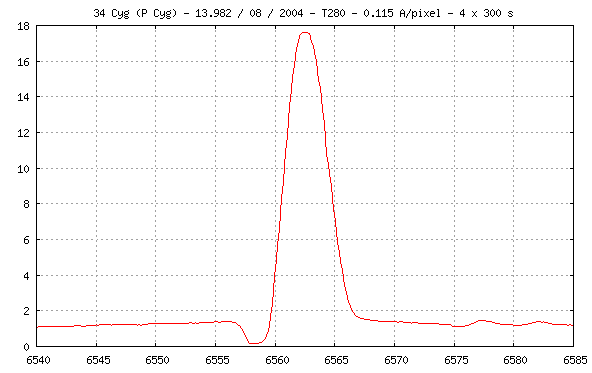
\includegraphics[scale=.40]{figures/34cygni.png}
\caption{The normalised spectrum of 34 Cygni around H$\alpha$.}
\end{figure}

It is hypothesised that distinct physical processes within these stars generate the respective line profiles \cite{hou2016catalog}. Beals was the first to demonstrate that P Cygni and Inverse P Cygni line profiles can be explained by the interaction between the stellar disk of a hot, massive young star and the expanding or contracting shell of gas surrounding the star \cite{1953PDAO....9....1B}. 

\begin{figure}[h]
\centering
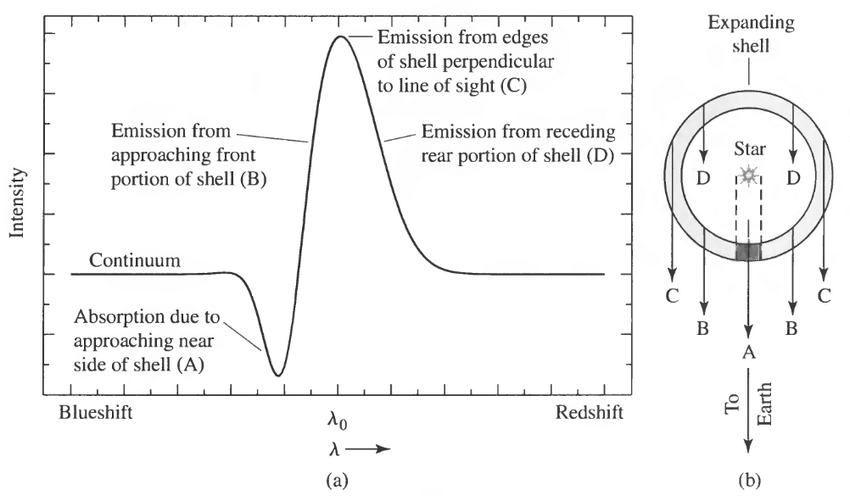
\includegraphics[scale=.40]{figures/expandingpcygni.png}
\caption{Cartoon depicting the physical mechanism by which a P Cygni line profile is generated. Reproduced from Kasai (2013)\cite{kasai2013type}.}
\end{figure}

The P Cygni line profile observed is thus a result of an expanding shell of gas around the main disk of the young hot star. The segment of this shell along the ling of sight contributes to the generation of the absorption line in the spectrum. An average or normal main sequence star will only show a significantly deep absorption line/trough near H$\alpha$. However, note that in the case of P Cygni, the regions B, C and D of the shell contribute to an emission line. This emission line can occur near H$\alpha$. As we move from B to C, the intensity of the emission line increases until we reach the edge of the shell. Beyond this point the shell is receding with respect to the line of sight and the intensity of the emission line decreases. It is believed that the opposite process occurs in the case of an inverse P Cygni star. In this case, the shell of gas is contracting and this inflow is responsible for the blue shifted emission line, often to the left of H$\alpha$.

\begin{figure}[h]
\centering
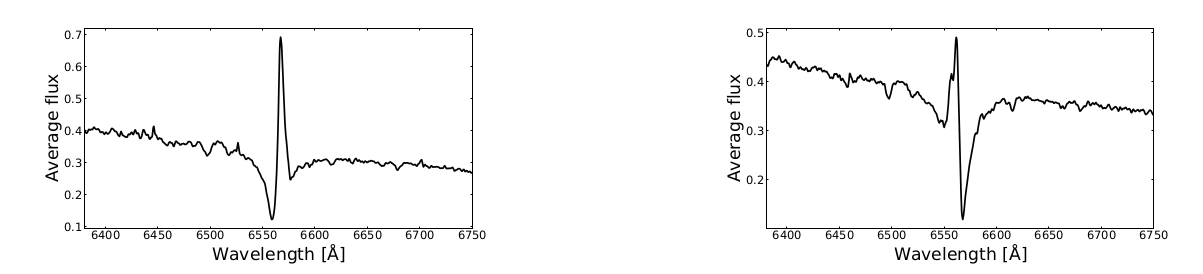
\includegraphics[scale=.50]{figures/p cygni and inverse p cygni.png}
\caption{A P Cygni spectrum (left) and an inverse P Cygni spectrum (right) from LAMOST Data Release 7. Reproduced from Zhang (2021)\cite{zhang2021catalog}.}
\end{figure}

\section{Morphological Classification}
One of the first modern attempts at identifying and characterising P Cygni stars was by Beals (1953) \cite{1953PDAO....9....1B}. This work compiled Northern Hemisphere observations of P Cygni stars into a comprehensive catalog. This catalog was compiled by examining spectra using the naked eye, during a period of observation between the years 1928 and 1946. The catalog was then used to generate hypotheses of how P Cygni stars may exchange material with their surroundings via accretions, inflows and outflows. The morphological properties of the spectra were then used to calculate the wind velocities of inflows and outflows. 

\begin{figure}[t]
\centering
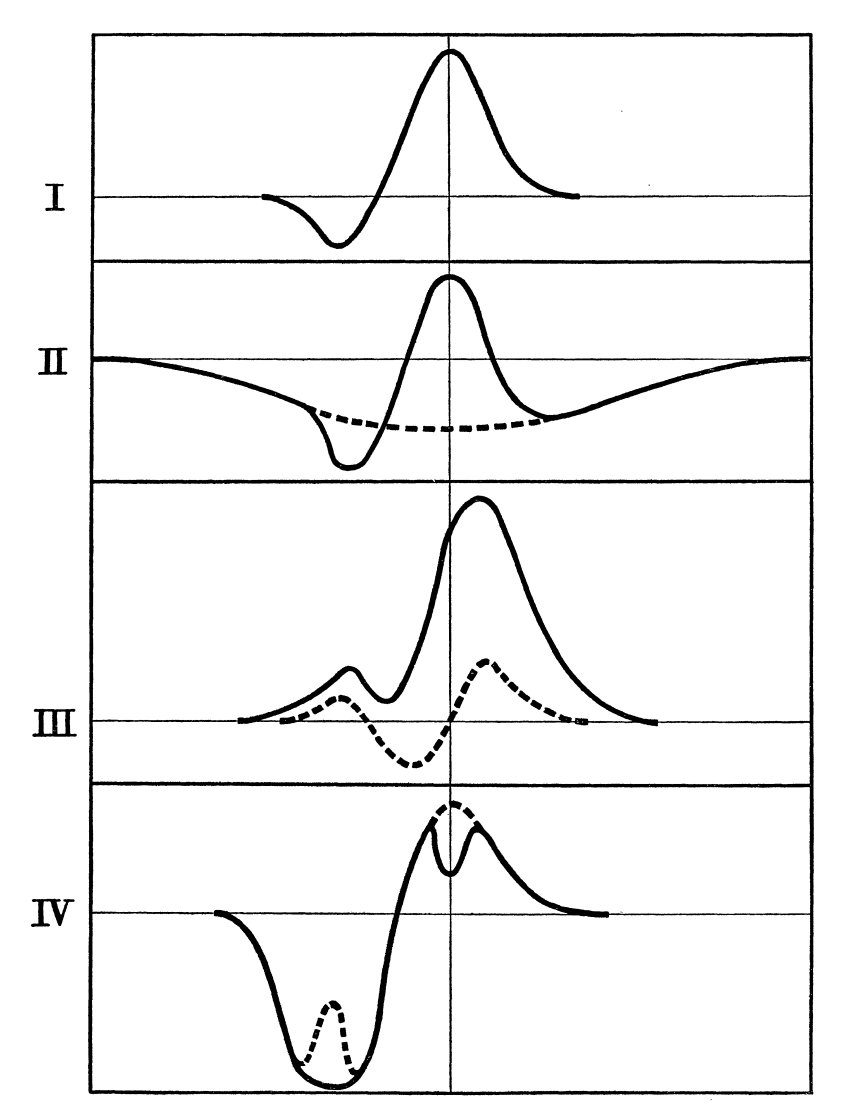
\includegraphics[scale=.30]{figures/beals class 1.png}
\caption{Primary P Cygni classes - the morphological classification of P Cygni spectra proposed by Beals (1953) \cite{1953PDAO....9....1B}.}
\end{figure}

The work also presents an early attempt at classification of P Cygni stars based on their morphologies. The classification provided by Beals is broader than modern schemes \cite{reipurth1996halpha}. In addition to the primary classes, Beals proposed a set of non-typical classes which were also considered to be P Cygni spectra. This work does not consider these non-typical classes to be P Cygni spectra but rather consider them to be a subgroup of emission line spectra. This approach is congruent with modern research \cite{vcotar2021galah}\cite{zhang2021catalog}\cite{reipurth1996halpha} which promote constraints on the classification of P Cygni and inverse P Cygni morphologies. 

Classification regimes since the 1950s have largely been manual i.e. visual inspection of spectra. However, over the last five to seven years semi-automated and automated methods have been explored by many groups. A more detailed discussion of these attempts are provided in Chapter 3.

\begin{figure}[h]
\centering
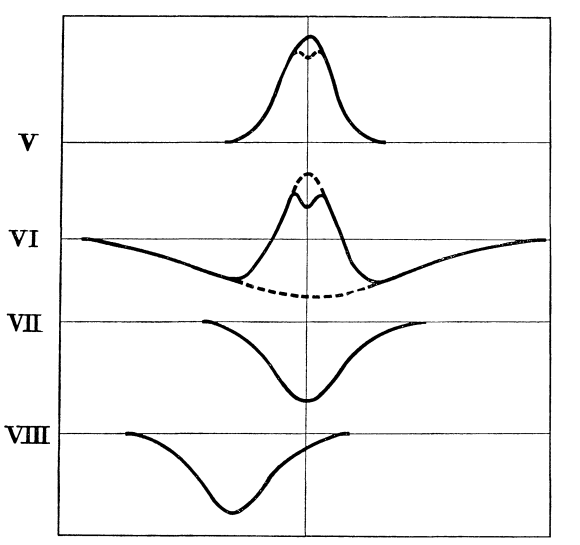
\includegraphics[scale=.50]{figures/beals class 2.png}
\caption{Non-typical P Cygni classes proposed by Beals.}
\end{figure}

\section{Importance}

The identification, classification and modelling of peculiar stars such as P Cygni and inverse P Cygni can provide significant insight into our understanding of stellar evolution and the physical processes that drive them. With the advent of modern large scale spectroscopic survey science, the importance of detecting these stars and modelling them using data driven methods has gained prominence.

Modern spectroscopic surveys generate data from millions of sources. These "million star surveys" generate a significant volume of data. Thus, it has become impractical to study these sources using manual methods. In order to generate stellar parameters from survey spectra, modern researchers rely on generalised automated pipelines. These generalised pipelines rely on templates and models that assume a non-peculiar baseline. 

It has been demonstrated that such an approach has an impact on the accurate determination of effective temperature \cite{cayrel2011halpha}\cite{amarsi2018effective}\cite{giribaldi2019accurate}. The effect on computing stellar masses has also been well documented \cite{ness2016spectroscopic}\cite{bergemann2016gaia}. Thus the identification and characterisation of peculiar stars such as P Cygni and inverse P Cygni stars has a direct impact on the accuracy of automated estimation of stellar parameters in large scale spectroscopic surveys. 

\section{The GALAH Survey}

The GALAH survey is a million star Milky Way spectroscopic survey which uses the HERMES spectrograph at the Anglo Australian Telescope \cite{de2015galah} \cite{buder2021galah+}. The GALAH survey is currently in its third data release (DR3) and contains more than 600,000 spectra. The volume of data being generated by the GALAH survey has necessitated the use of semi-automated and automated data analytics pipelines over manual methods.

\section{Goals}

REWRITE THIS

This thesis will use a novel data driven approach to cluster, classify and identify PCT stars in GALAH DR3. Once these PCT stars have been identified, the thesis will characterise these stars with reference to stellar parameters. This thesis will model the spectra using optimisation techniques and gaussian mixture models (GMM) to estimate the stellar wind velocity directly from the normalised spectra of the PCT stars (Zhang et al. 2021; Traven et al. 2015).

The focus of this literature review is twofold. One aspect of the review will be on the scientific work done on P-Cygni stars in particular and emission stars in general, and their relevance to the thesis. The second aspect will be a brief survey of recent computational methods that are relevant to the thesis, with a special focus on machine learning and signal processing methods. 





% Data
\chapter{A Review of Methods To Date}

The GALAH survey is not biased towards emission-line stars and it is expected that a majority of spectra are typical. This places a constraint on the methods that can be used to identify emission-line spectra. Methods, both manual and automated, must be adapted to detect anomalies or outliers in data to separate emission-line spectra from more typical spectra. In this work, identifying emission-line spectra in large scale surveys is presented as a pre-processing step to classification and forms a critical step in the novel method presented in Chapter 6. This chapter presents essential background material and a review of methods that have been used to identify H$\alpha$ emission-line spectra, in both smaller-scale observations during the latter half of the 20th century as well as more modern large-scale surveys in the early 21st century. These methods have also been placed in the context of their importance in the identification and classification of P Cygni, inverse P Cygni and other emission-line spectra.

\section{A Historical Perspective}
Chapter 1 introduced the work of Beals who pioneered the study of emission-line stars in the 20th century. The work was manual and time consuming and took the researcher decades to compile with the assistance of a team that included secretaries and draftspersons. Despite these efforts, the catalogue of data compiled in 1953 was small by modern standards. This work could not identify more work in literature that focused on identifying and classifying emission-line stars until the late period of the 20th century. This is potentially due to the significant amounts of labour required to carry out these projects in the absence of modern data mining methods. 

In 1993, an atlas of high resolution line profiles with H$\alpha$ emission-line spectra was provided by \citet{van1993atlas}. The authors note that the radial velocities of the 59 emission lines considered were generally red-shifted. They provide a classification scheme for H$\alpha$ spectra based on their morphology, devised entirely by using manual methods. More specifically, direct visual inspection and measurement of the width and shape of the line profile was used to classify these spectra. In particular, wind velocity dispersion outside the primary disk of the star was used to determine the membership of spectra in each class.

\begin{figure}[!htb]
\centering
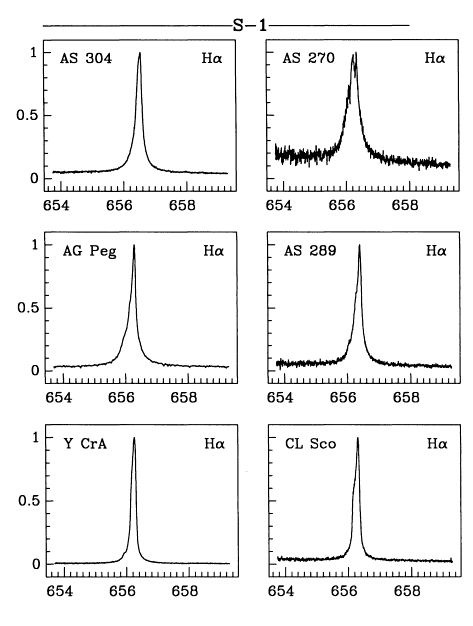
\includegraphics[scale=0.75]{figures/van winckel class.png}
\caption{Sample spectra from sub-type S1 as classified by Van Winckel et al.}
\end{figure}

\begin{figure}[!htb]
\centering
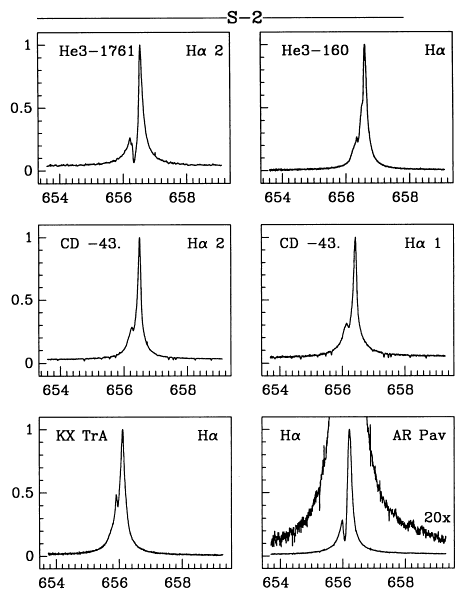
\includegraphics[scale=0.75]{figures/van.png}
\caption{Sample spectra from sub-type S2 as classified by Van Winckel et al.}
\end{figure}

A few of the classes identified by the authors include sub-type S1, which are narrow emissions with no prominent absorption; sub-type S2, which shows a clear absorption feature superimposed on a broad emission feature; and sub-type S3 which shows a strong absorption feature which reaches at least the continuum level. S3, which shows the smallest wind velocity dispersion, thus demonstrating the relationship between the morphology of the spectra and the physical processes that generate them.

\begin{figure}[!htb]
\centering
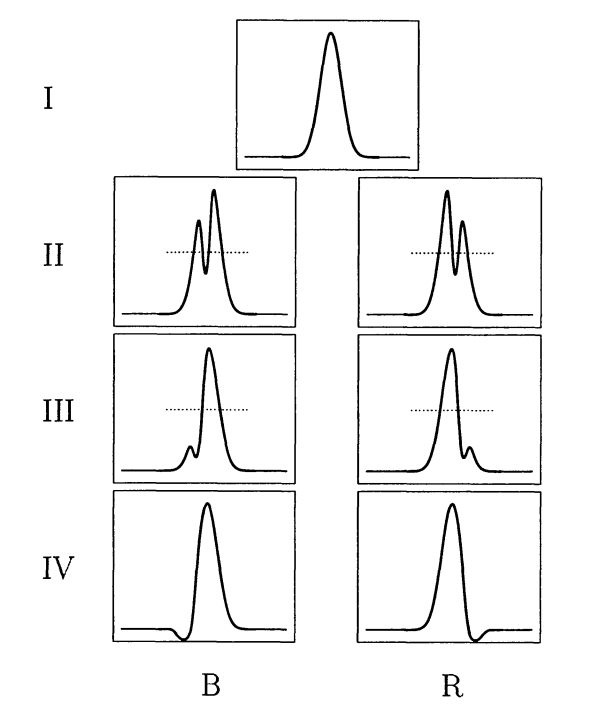
\includegraphics[scale=1]{figures/reipurth classes.png}
\caption{The morphology based classification scheme proposed by Reipurth et al. (reproduced). Depending on the location of the primary peak in relation to the secondary peak, the letters B and R were appended to the Roman numerals. They stand for blue-shifted and red-shifted respectively.}
\end{figure}

Following on three years later, in 1996, Reipurth et al. studied the H$\alpha$ emission-line profiles of pre-main sequence stars using manual methods. In addition to identifying T Tauri stars and Ae\symbol{92}Be stars using high resolution spectra (R$\sim$50,000), the study focused on the morphological properties of P Cygni stars, as well as the physical processes that generate them. The study notes the discovery of complex morphological profiles among the T Tauri, Ae\symbol{92}Be and P Cygni stars \citep{reipurth1996halpha}.

The authors proposed a two dimensional classification scheme based on the relative height of a secondary peak compared to the primary peak, and whether the absorption line is blue or red shifted. The authors noted the classification of 25\% symmetric profiles, 49\% blue shifted absorption profiles and 5\% P-Cygni profiles in the observed spectra. Of the spectra, 21\% fall into the red-shifted absorption category. In addition to this morphological classification, the authors also presented wind velocities of the samples with some stars recording extremely high velocities of $\sim$900km/s. 

The classification of P Cygni stars in Reipurth et al. follows the scheme proposed by Beals. The authors have also presented a discussion comparing observed data to models in literature, particularly models that constrain mass, radii and photospheric temperatures. No specific model details for P Cygni stars were provided. Further catalogues of H$\alpha$ emission-line stars have been provided by \citet{kohoutek1999catalogue}. These catalogues contain 98 identified emission-line stars in the Northern Milky Way. These catalogues do not specifically identify P Cygni stars or inverse P Cygni stars.

Working with data from NGC 6611, in 2013, Bonito et al. note that for stars surrounded by active disks, the morphology of the emission lines could fall into categories such as symmetric with broad wings, asymmetric and, in extreme cases, P Cygni and inverse P Cygni. The authors have used the classification scheme proposed by Reipurth et al. mentioned above and have adhered to the type I - IV scheme with B and R suffixes to denote blue-shifted and red-shifted emission lines respectively \citep{bonito2013spectroscopic}.

 \citet{traven2015gaia} presented a catalogue of H$\alpha$ emission-line stars in the Gaia-ESO survey. This survey is biased towards young open clusters and consequently, the authors note a relatively large proportion of H$\alpha$ emission-line spectra that were identified in this work. The authors note the identification of 3765 emission-line stars from a sample of 22,035 spectra. This work is notable as it uses a combination of empirical rules and automated methods like spectral fitting to sort the H$\alpha$ emission-line spectra into eight distinct morphological categories: single–component emission, emission blend, sharp emission peaks, double emission, P-Cygni, inverted P-Cygni, self–absorption, and emission in absorption. This work was briefly presented in Chapter 1. 

\begin{figure}[!htb]
\centering
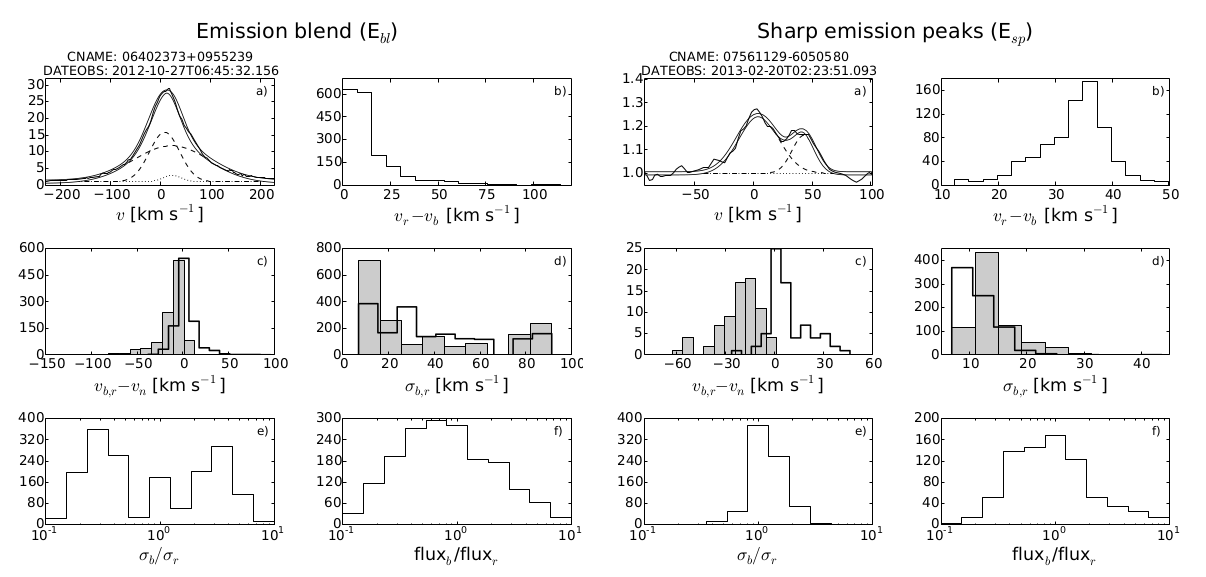
\includegraphics[scale=.50]{figures/gaia eso1.png}
\caption{Classes of emission-line spectra identified in the Gaia-ESO Survey. Reproduced from Traven et al.}
\end{figure}

\begin{figure}[!htb]
\centering
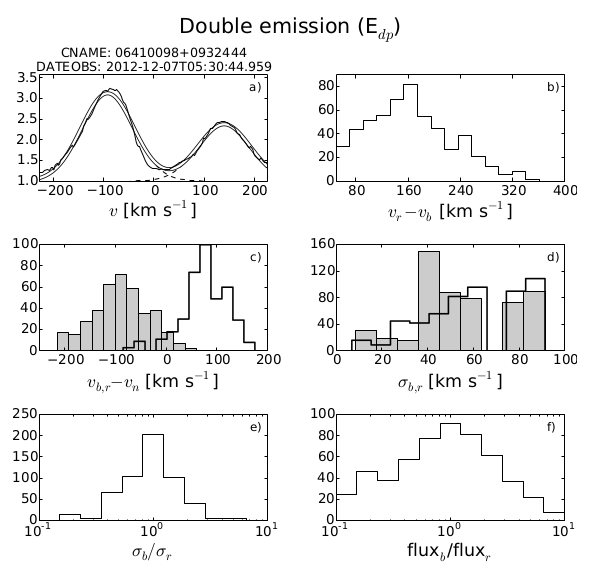
\includegraphics[scale=.50]{figures/gaia eso2.png}
\caption{Classes of emission-line spectra identified in the Gaia-ESO Survey. Reproduced from Traven et al.}
\end{figure}

The Gaia-ESO survey had conducted repeat observations of about half the identified H$\alpha$ emission-line stars. Thus the authors were able to comment on the temporal variability of these stars. The conclusion was that while some morphological categories exhibited stability of their spectral profiles over time, P-Cygni and self-absorption profiles may not. Supplementary information of these spectra from SIMBAD, VizieR and ADS were also provided. In addition to this data, the authors have provided wind velocity estimates based on the curve fitting procedure. The authors note that the identification, classification and characterisation of emission-line stars can be valuable for automatic pipelines in large surveys, where they can pinpoint outliers when calculating general stellar properties and abundances. Additionally, they note that the identified stars can be used in studies of star formation processes, interacting binaries and related fields of stellar physics. 

This work draws several conclusions from this historical perspective,

\begin{enumerate}
\item These methods relied exclusively on visual inspection of spectra and manual methods to identify H$\alpha$ emission-line spectra. While this may have been a suitable approach in the past, it is extremely challenging to extend and scale these methods to data sets generated by million star all-sky surveys in the modern era.
\item It was demonstrated in Chapter 1 that the variety of spectral morphologies are hypothesised to be generated by distinct physical phenomena linked to the stellar disk and the gas that surrounds it. Thus morphology-based classification approaches as demonstrated by Reipurth et al. and Beals are important in the context of developing a greater understanding of stellar evolution and dynamics.
\item Finally, these studies have identified P Cygni and inverse P Cygni (among other classes of spectra) as a subset of H$\alpha$ emission-line spectra. The current work takes this fact to its logical conclusion i.e. the probability identification of P Cygni and inverse P Cygni spectra can be increased if the search space and feature space of the raw data can be reduced from the complete DR3 catalogue to a much narrower subset of H$\alpha$ emission-line spectra during pre-processing. 
\end{enumerate}

\section{Recent Developments}
The increase in data availability via large scale spectroscopic surveys has necessitated and demanded the use of automated identification and classification methods. More recently, these methods have included statistical analysis and machine learning. In general, machine learning approaches can fall into two categories; supervised and unsupervised learning. The former relies on the availability of a suitably robust set of training examples, while the latter attempts to generalise and learn from unlabelled data \citep{hastie2009elements}. 

While a full discussion and review of machine learning methods is beyond the scope of this thesis, the methods that are relevant to this work are presented in subsequent chapters, with Chapter 4, in particular, presenting a more detailed discussion on methods that are relevant to this work. This section following reviews four recent methods that use machine learning to identify spectra in large surveys and discusses their strengths and limitations.

\subsection{Applying K-means Clustering Directly on Data from APOGEE}
The goal of k-means clustering to partition a set of observations into a predefined set of clusters. Each observation would belong to a cluster with the nearest mean which serves as the centroid or prototype of the cluster \citep{macqueen1967some}. Formally, given a set of $n$ observations such as \(x_1,x_2,...,x_n\) where each observation is a $d$ dimensional vector, the algorithm will partition the $n$ observations into $k$ sets $S=\{S_1,S_2,...,S_k\}$ such that the intra-cluster variance is minimised. This objective can be represented as,

\begin{equation}
{\underset {\mathbf {S} }{\operatorname {arg\,min} }}\sum _{i=1}^{k}\sum _{\mathbf {x} \in S_{i}}\left\|\mathbf {x} -{\boldsymbol {\mu }}_{i}\right\|^{2}={\underset {\mathbf {S} }{\operatorname {arg\,min} }}\sum _{i=1}^{k}|S_{i}|\operatorname {Var} S_{i}
\end{equation}

where $\mu_i$ is the mean of the points in $S_i$. 

Using the identity,

\begin{equation}
    |S_{i}|\sum _{\mathbf {x} \in S_{i}}\left\|\mathbf {x} -{\boldsymbol {\mu }}_{i}\right\|^{2}=\sum _{\mathbf {x} \neq \mathbf {y} \in S_{i}}\left\|\mathbf {x} -\mathbf {y} \right\|^{2}
\end{equation}

it can be shown that this is equivalent to minimising the pairwise squared deviations of points belonging to the same cluster.

\begin{equation}
{\underset {\mathbf {S} }{\operatorname {arg\,min} }}\sum _{i=1}^{k}\,{\frac {1}{|S_{i}|}}\,\sum _{\mathbf {x} ,\mathbf {y} \in S_{i}}\left\|\mathbf {x} -\mathbf {y} \right\|^{2}
\end{equation}

This method was used on high resolution APOGEE data (R$\sim$22,500), which is part of the Sloan Digital Sky Survey (SDSS) \citep{eisenstein2001spectroscopic, blanton2017sloan}. In the absence of labelled training samples in the APOGEE survey, Garcia-Dias et al. used k-means to cluster similar spectra into distinct groups \citep{garcia2018machine}. Each spectrum produced by APOGEE was treated as a $d$-dimensional vector. The number of observations $n$ was the number of spectra generated by APOGEE, which was approximately 150,000. $k$ was set to 50, presumably by a process of trial and error. The authors note that they were able to separate dwarfs, sub-giants, RC and RGB stars using this approach. The authors also add that the approach is sensitive to initialisation, and thus sensitive to the number of clusters $k$. One major limitation of this approach is that a discrete classification in the flux space does not result in a neat organisation in the parameters' space, which implies that the authors' were not able to link spectral features such as morphologies to the machine learning parameter space. The other limitation is the manual sorting of clusters that reduced the number of clusters from 50 to 9. This implies that certain spectra were incorrectly clustered by the k-means algorithm. Notable, the authors were unable to cluster H$\alpha$ emission-line spectra using this method. 

The primary conclusion that can be drawn from this work is that k-means clustering, while robust on more traditional machine learning tasks, may perform poorly if it is used to cluster and ultimately classify morphologically-similar spectra such as P Cygni, inverse P Cygni and other emission-line classes identified using manual methods. A method that relates the flux space, and consequently the morphology of the spectrum to a parameter space may perform better than k-means. 

\subsection{Combining Machine Learning and Manual Methods on Data from the LAMOST Survey}

The LAMOST survey is a low resolution spectroscopic survey with 10 million Milky Way stars as potential survey spectra. \citet{zhang2021catalog} were able to use a training and test set (labelled spectra) comprising of 5915 samples for spectral classification. This training set was based on data released by \citet{hou2016catalog}, who developed the data set by using a combination of empirical rules and visual examination of 10,000 LAMOST spectra. The existence of labelled data including seven P Cygni and inverse P Cygni spectra identified by Hou et al. was used by Zhang et al. for supervised machine learning algorithms. Ten different supervised learning methods were then applied to this data set including including KNN (K-Nearest Neighbor), RF (Random Forest), AdaBoost, Naive Bayes (MultinomialNB, GaussianNB, BernoulliNB), logistic regression, SVM (Support Vector Machine) and Artificial Neural Network (Single-hidden Layer, Three-hidden Layer). A comparison of the performance of these methods was not provided by the authors. A detailed discussion of these methods is omitted as it would be beyond the scope of this thesis. 

Zhang et al. note that the k-nearest neighbour and random forest methods outperformed all other methods. These two supervised machine learning models were then applied to 498,588 spectra resulting in 56,574 potential H$\alpha$ emission-line spectra. These spectra were then visually inspected with a final candidate list of 30,048 H$\alpha$ emission-line spectra. Despite the use of a number of machine learning methods, the authors fell back on manual visual inspection of spectra in building the training set, and during the classification of the identified potential H$\alpha$ emission-line spectra. Thus it is clear that machine learning methods must be applied carefully in order to achieve the desired end goals such that the work does not need to fall back on using manual methods.

\subsection{Dimensionality Reduction in Action: Using t-SNE to Classify GALAH Spectra}

It is often helpful to transform the data from a high-dimensional space to a low-dimensional space while ensuring that meaningful features of the original data are preserved. In the case of P Cygni and inverse P Cygni spectra, these meaningful properties would presumably include some information about the morphology of the spectrum although this may not be guaranteed. A stellar spectrum of vector length $d$ (a wavelength grid of size $d$) can be used to create a vector space of dimensionality equal to $d$. In the case of GALAH DR1 this value is $\sim$4500. Conducting computational operations such as clustering and classification on a higher dimensional vector space of size $\sim$4500 can be challenging as it introduces significant computational overheads. In addition to the curse of dimensionality, which will be detailed in Chapter 3, researchers would also face practical limitations due to the computational intractability of working on higher dimensional vector spaces.

Principal component analysis (PCA) is arguably the most well known dimensionality reduction method. However, PCA may not be suitable in the context of GALAH DR1, and certainly DR3, since these data sets are biased towards non-emission line spectra. A PCA-led approach may select features that represent the absorption-line, while emission-line features may be ignored. This hints at a possible outlier or anomaly detection-based approach to emission-line spectra identification. This work will revisit this idea in Chapter 6.

More recent and novel dimensionality reduction methods such as t-distributed stochastic neighbour embedding (t-SNE) \citep{van2008visualizing} have been used on spectral data from GALAH DR1 \citep{traven2017galah}. Given a vector of size $d$, the application of the t-SNE algorithm will project this vector space onto a 2-dimensional vector space. The distances between data points on this 2-dimensional vector space can then be used to cluster similar data points into similar groups using a variety of popular clustering methods such as DBSCAN \citep{ester1996density} or HDBSCAN \citep{campello2013density}. A detailed discussion of this method and its suitability to this work is presented in Chapter 5.

\begin{figure}[!htb]
\centering
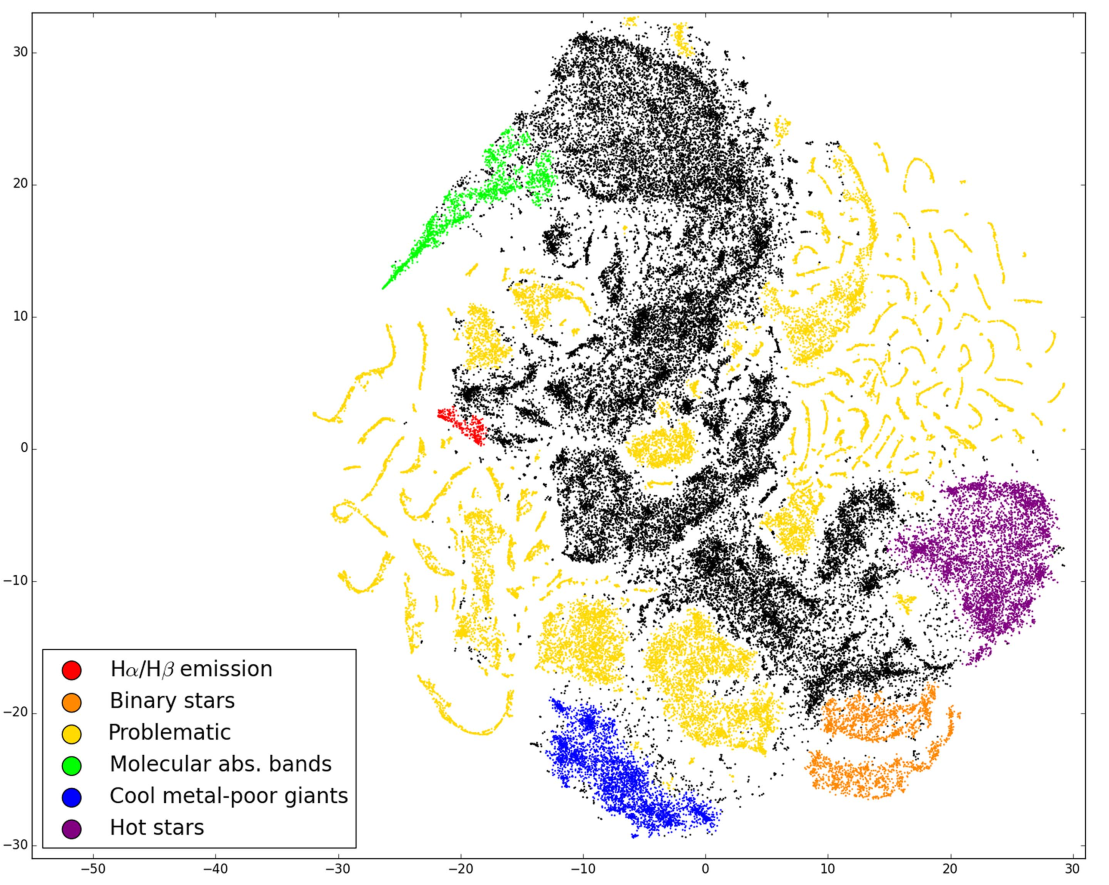
\includegraphics[scale=0.36]{figures/tsne traven.png}
\caption{The t-SNE plot with classified regions reproduced from \citet{traven2017galah}. The x and y axes do not have a physical meaning but serve as spanning vectors for the 2-dimensional space.}
\end{figure}

Using this method, Traven et al. classified six distinct stellar types and identified H$\alpha$ and H$\beta$ emission-line spectra in GALAH DR1. These spectra were further examined and 18 P Cygni spectra were identified. The identification of P Cygni spectra was a sub-component of a broader study of stellar types in GALAH DR1. The authors note that the number identified was lower than expected which implies that there is significant scope to develop methods capable of detecting a larger number of emission-line stars in the GALAH survey. Crucially, this method was not able to separate P Cygni spectra from double peaked spectra, emission superimposed on absorption and other emission-line spectra. When examining the t-SNE plot above, it is clear that the authors were not able to distinctly separate the H$\alpha$ emission-line stars as a distinct cluster from the unclassified region (black) but rather fell back on manual tagging of this region on the projection space. 

Dimensionality reduction can overcome problems such as computational intractability but this should not be at the cost of information losses related to the morphology of the spectrum. Since these morphologies uniquely identify the spectral types, a significant loss of this information will lead to poor classification performance. This work will revisit this in detail in Chapter 5 and provide examples using t-SNE where this type of information loss may have occurred.

\subsection{Neural Networks as Anomaly Detectors: Using an Autoencoder on Data from GALAH and Other Surveys}

In contrast to t-SNE, Čotar et al. introduced an anomaly detection based approach to identify emission-line stars, the performance of which was a significant improvement over the t-SNE based method described in the prior section. This method used an autoencoder (AE), which is a type of artificial neural network (ANN) that takes input data and reduces it to a pre-selected number of "latent features" that inhabit a low-dimensional vector space known as the latent space. The latent space can capture important features that exist in the original $d$-dimensional vector space. By processing $n$ samples of $d$-dimensional vectors, the autoencoder can then learn the latent space representation of the higher dimensional features. This is known as encoding. In the next portion of the network, the network then attempts to recover the original data from the latent vector space. The process that reduces a $d$-dimensional vector and vector space to a vector space of size $p$<$d$ is a dimensionality reduction process similar to PCA or t-SNE. The portion of the network that takes a $p$-dimensional vector from the latent space and projects it back to a $d$-dimensional vector space is essentially the inverse process of the dimensionality reduction procedure. This is known as a decoder. Since the original data is generated from the latent space, autoencoders fall into a class of ANNs called generative models (generative ANNs). Note that the latent space for an autoencoder is discrete. ANNs that can generate continuous latent spaces in this manner are known as variational autoencoders (VAEs) and are beyond the scope of this work. 

Autoencoders are widely used in anomaly detection applications \citep{sakurada2014anomaly} and can be suitably adapted to detect atypical spectra from survey data that contains a majority of typical spectra. If the autoencoder model is trained on non-anomalous data ("normal" data), the model will learn the latent space representation of non-anomalous data. Subsequently, if an anomalous data point is passed through the model, the autoencoder will attempt to generate this data from the latent space representation it has learned. Since the learned model was trained on non-anomalous data, the autoencoder will generate an inaccurate representation of the anomalous data. This leads a prediction error which can be used as a flag to detect time-series as well as non time-series anomalies in data.

The GALAH survey is a general all-sky survey that can be expected to generate a significantly higher proportion non-anomalous spectra. Since DR3 is not biased towards young, violent, hot stars or stellar nurseries, we expect a significantly higher proportion of spectra to show "typical" (non-anomalous) H$\alpha$ line profiles and indicate absorption. In this regime, an H$\alpha$ emission-line, and consequently, P Cygni and inverse P Cygni spectra are rare and anomalous. If an autoencoder is trained on "normal looking" spectra which do not show emission lines near H$\alpha$, it can be sensitive to H$\alpha$ emission-line spectra. 

\begin{figure}[!htb]
\centering
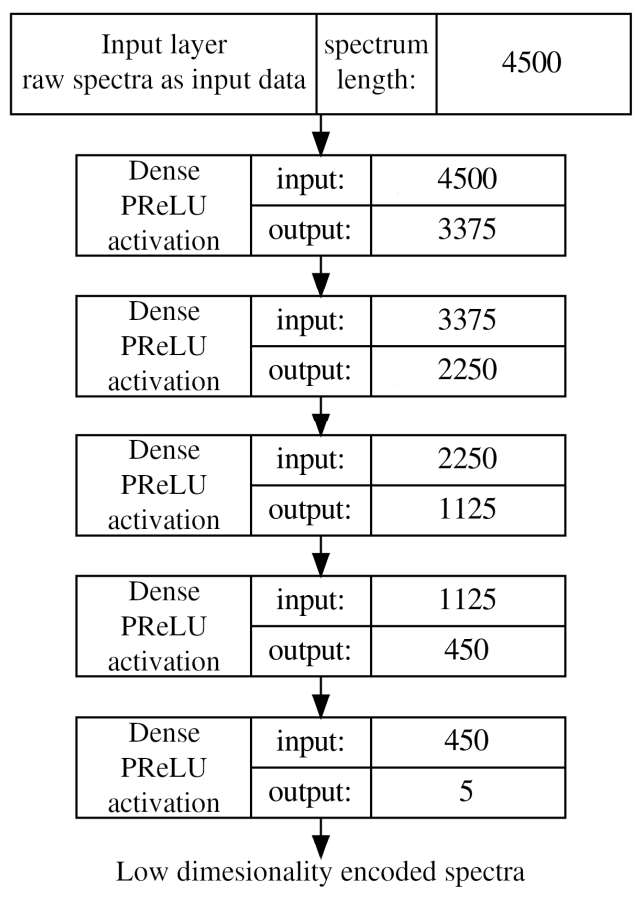
\includegraphics[scale=0.45]{figures/autoencoder.png}
\caption{An autoencoder architecture capable of detecting H$\alpha$ emission-line spectra from DR3. Reproduced from Čotar et al.}
\label{fig2.7}
\end{figure}

This method was used by Čotar et al. to detect H$\alpha$ emission-line spectra in DR3 and other surveys \citep{vcotar2021galah}. The authors chose a network architecture that reduces a $d$-dimensional DR3 spectrum to a $p$-dimensional latent space representation. Here, $d$ = 4500 while $p$ = 5. Presumably, $p$ was set to 5 to potentially capture the primary stellar parameters and represent them within the latent space. The intervening layers and the final architecture that is capable of detecting H$\alpha$ emission-line spectra is presented in Figure \ref{fig2.7}. The authors did not further classify and detect P Cygni, inverse P Cygni and emission-line spectra using this method. 

\section{Concluding Remarks}

It is clear from the review presented here that given the scale, modern work should rely heavily on automated methods when identifying atypical spectra such as those of emission-line stars. Attempts have been made at using machine learning methods to tackle this problem over the last five years with varying levels of success. If labelled data is available, supervised machine learning methods can be applied as in the case of Zhang et al. However, these methods must be applied more judiciously if progress is to made with regards to relying on human beings to detect atypical spectra in large-scale surveys.

Regarding P Cygni stars and inverse P Cygni stars specifically, the literature is sparse and the available samples are few. For example a catalogue of these spectra and stars do not exist at present. This can limit the use of supervised machine learning methods and more importantly, can limit the science work that has been conducted on these spectra in the literature. Thus improvements to methods and the introduction of novel methods can lead to more emission-line spectra being identified and classified which in turn can lead to new science work on these stars. 

The use of machine learning has been a relatively new development in the field. As far as this author is aware, the use of t-SNE in 2017 is the first instance of using machine learning to identify and classify H$\alpha$ emission-line spectra. However as this work will demonstrate in Chapter 5, it can be challenging to use t-SNE to classify P Cygni and inverse P Cygni spectra. Dimensionality reduction methods must be chosen carefully so as they do not lose too much discriminatory information with regards to the features of the emission-line spectra.

Taking an anomaly detection or outlier detection approach such as Čotar et al., and using a neural network architecture such as an autoencoder can be beneficial in reducing the search space of surveys such as GALAH from the total spectra available to only the potential emission-line spectra. However this method cannot be used to classify particular types and sub-species of emission-line stars such as P Cygni and inverse P Cygni. Similar to dimensionality reduction, this method can reduce the complexity of the problem by allowing the researcher to focus on only the most relevant data points when attempting to identify and classify emission-line spectra. Combined with other methods, this method can serve as a pre-processing step when identifying and classifying emission-line spectra. This work explores this idea fully in Chapters 4 and 6. 

Finally, popular unsupervised machine learning methods such as k-means as well as supervised machine learning methods such as logistic regression may not be suitable. The latter requires labeled training data which this work did not posses. There exists evidence in literature that the former performed poorly on the task of identifying and classifying emission-line stars in a large scale spectroscopic survey in 2018 \citep{garcia2018machine}. Due to time constraints, this work did not evaluate and consider these methods further.



% Halpha
\chapter{The Data Used in This Work}

This chapter presents an overview of the raw data used in this work, the challenges faced when working with higher dimensional data, strategies that were used to overcome these challenges and notes on data re-sampling and spectra region selection. Furthermore, it presents a recent data set of emission-line stars that aided the development of the methods presented in subsequent chapters of this work.

\section{Data Acquisition}

This work utilises the most recent open access spectral data from the GALAH survey. At the time of writing, the GALAH survey is in its third data release (GALAH DR3). GALAH DR3 (hereafter DR3) comprises of 678,423 spectra for 588,571 stars, of which approximately 80\% are within a radius of 2 kpc \citep{buder2021galah+}. DR3 provides continuum normalised spectra and errors for a majority of candidates. Of the 588,571 stars, continuum normalised spectra of 588,343 have been provided. In the case of problematic reductions, for spectra where this is not possible, object IDs and flags have been provided. This study avoids using these problematic spectra.

The data is organised as individual \texttt{.fits} format files. Each file contains an object ID prefix (known as an \texttt{sobject\_id}) followed by the last digit in the filename which serves as a suffix for the camera number. Thus, the file \texttt{1705090057010093.fits} is a data file for an object with \texttt{sobject\_id=170509005701009} and contains spectral data from camera 3 (or the red camera). The blue, green and infrared cameras are denoted by the suffix 1, 2, and 4 respectively.
The red camera of the HERMES spectrograph is the spectral channel with the range 6478\r{A} - 6737\r{A} \citep{sheinis2014first}. This range is of particular interest to this work as the characteristic H$\upalpha$ line appears within this range. These individual files totalling 385 GB were downloaded to a Macquarie University file server and served as the data source for all work presented in this thesis.

\begin{figure}[!htb]
\centering
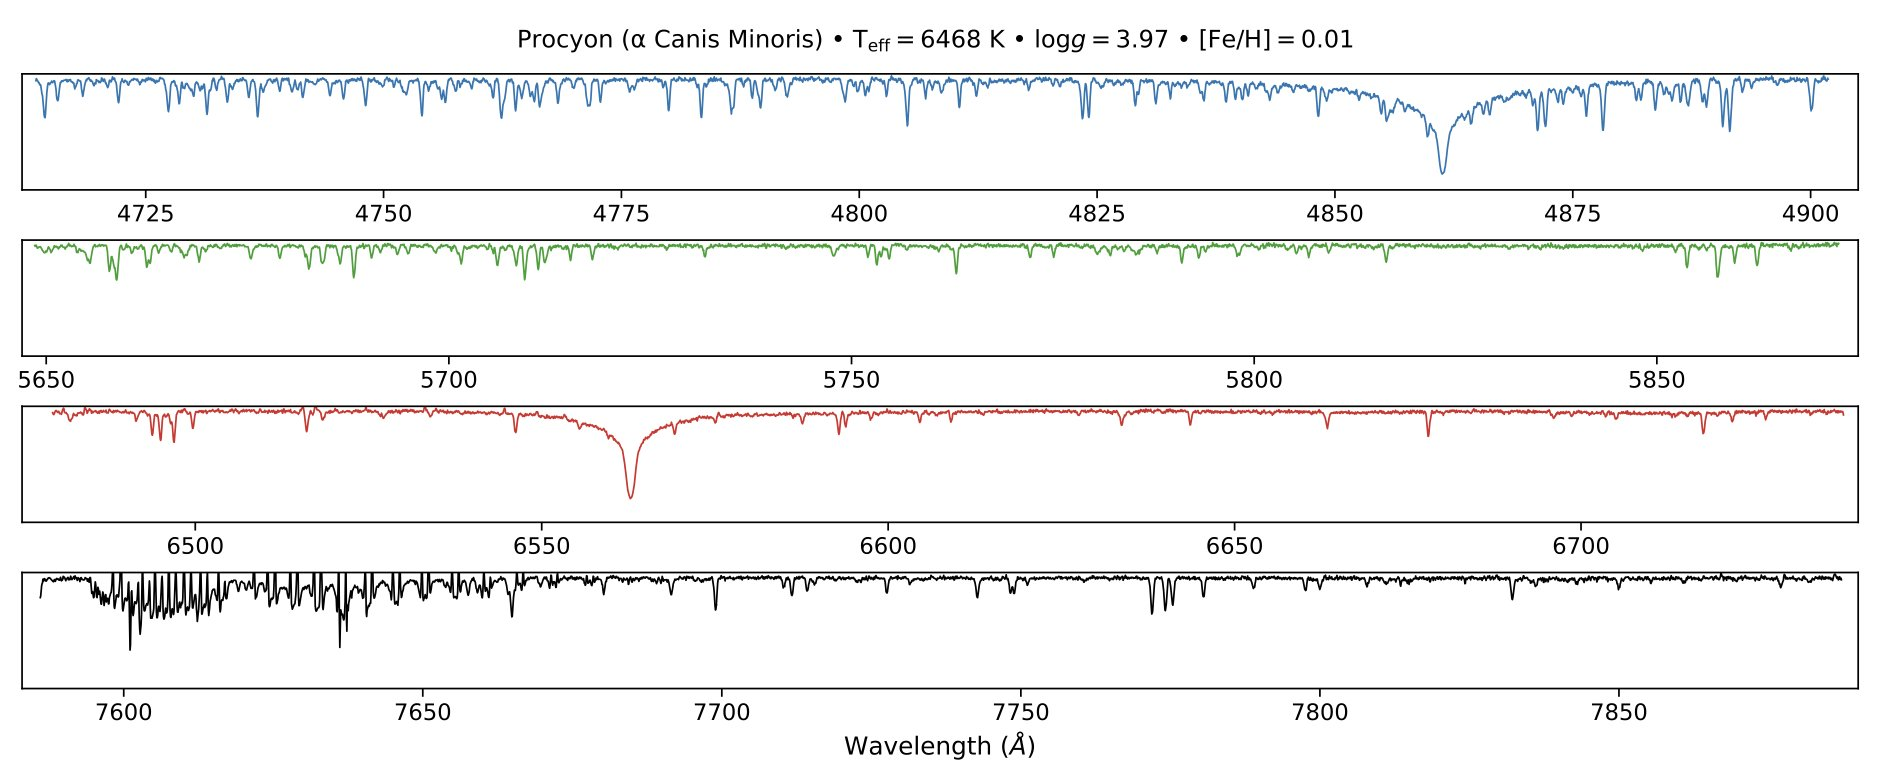
\includegraphics[scale=.25]{figures/galah cameras.jpeg}
\caption{All camera, normalised DR3 spectral data for the star $\upalpha$ Canis Minoris.}
\end{figure}

Feature exploration and engineering is a crucial step when conducting data analysis and in particular for preparation of data prior to the application of machine learning methods. This section provides an analysis of the feature space and search space of DR3 in the context of identifying emission-line stars. The results of this exploratory analysis placed constraints on the design of the machine learning methods discussed in subsequent chapters. Given that spectral features are recorded across four cameras at high resolution, the feature space of DR3 is significant. 

As an illustrative example, consider the red camera only. The feature space calculation is as follows,
\[\lambda_{min} = 6478\]
\[\lambda_{max} = 6737\]
\[\Delta\lambda \approx 0.06\]
$\Delta\lambda$ is the wavelength separation equivalent of the sampling rate of the wavelength grid. Thus the size of the wavelength grid is given by, \[N_{\lambda} = (\lambda_{max}-\lambda_{min})/\Delta\lambda \approx (6737-6478)/0.06 \approx 4317\]
This is the number of features in the red camera for a given spectrum, \[N_{f} \approx 4317\]
Thus the total number of features for the red camera across all available DR3 data is, \[N_{T} \approx 4317\times678,423 \approx \num[round-precision=2,round-mode=figures,
     scientific-notation=true]{2928752091}\]

This calculation naively implies the existence of a billion scale feature space, and consequently a potential billion dimensional vector space. This indicates that the data analysis and machine learning strategy should be planned and managed carefully. If care is not taken during feature engineering and pre-processing steps, the volume of data and complexity will lend itself to what is colloquially referred to as the "curse of dimensionality", which refers to the extraordinarily rapid growth in the difficulty of problems as the number of variables (or the dimension) increases \citep{kuo2005lifting}.

\begin{figure}[!htb]
\centering
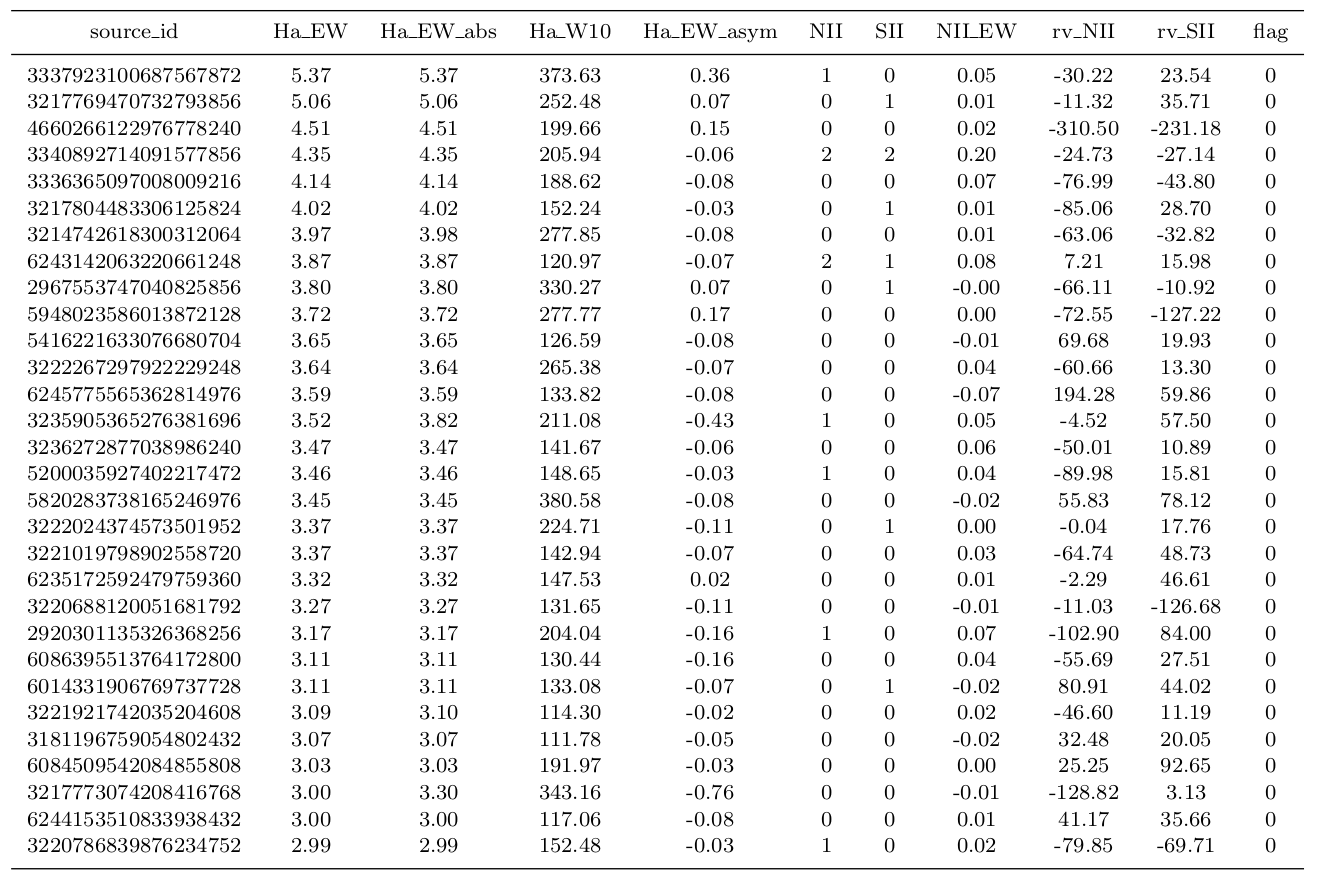
\includegraphics[scale=.45]{figures/cotartable.png}
\caption{The 30 strongest emitters. Reproduced from Čotar et al. \citep{vcotar2021galah}.}
\end{figure}

This work will also utilise a recently published data set of H$\upalpha$ emission line spectra. Published in 2020, Čotar et al. \citep{vcotar2021galah} used a prior version of the GALAH survey \citep{de2015galah}, the K2-HERMES survey \citep{wittenmyer2018k2} and the TESS-HERMES survey \citep{sharma2018tess} to derive a catalogue of potential H$\upalpha$ emission-line spectra using a specific type of neural network known as an autoencoder. Combining data from three surveys, this study used 669,845 continuum normalised stellar spectra as a data input source and included a small fraction of repeated observations. 

The study identified 10,364 emission-line spectra with varying degree of H$\upalpha$ emission components and sub components. Summarised information of these spectra, their object IDs, including GALAH DR3 \texttt{sobject\_ids} were released via \href{https://cdsweb.u-strasbg.fr/}{CDS} as open access data. This summarised data, excluding the continuum normalised spectra, was presented as a single \texttt{.fits} format file. In Chapter 4, this work will demonstrate that a novel clustering approach can identify P Cygni and inverse P Cygni spectra and other species from this sample. Furthermore, this data set was used to benchmark a well established dimensionality reduction based clustering method called t-SNE. These results are presented in Chapter 5. Given the significantly smaller feature and search space, exploring and prototyping methods on this data set proved extremely beneficial when developing the full machine learning method presented in Chapter 6.

\section{Interpreting Spectra as Time Series}

This work takes a unique view of continuum normalised spectra from DR3, casting and interpreting these as one would do a set of time series data points. This proved extremely useful as a mental model when developing the methods presented in this work. This section provides some insights into the motivation for using this mental model. 

A plot of flux recorded by each camera, when presented as a function of wavelength, can be treated mathematically as traditional time series data. While a monotonically increasing time axis is not included in the DR3 data, the monotonically increasing wavelength grid can serve as an analogue to the time axis. Morphologically, the variation of normalised flux against a wavelength grid is analogous to a variable plotted against a time grid \citep{nielsen2019practical}.

This work takes inspiration from this approach. This is an unconventional yet incredibly powerful approach to analysing stellar spectra. Precedent for this approach can be found in related fields such as chemistry and nuclear magnetic resonance (NMR) spectroscopy where NMR spectra are subjected to signal processing methods originally developed for time series analysis \citep{nielsen2019practical}. Viewing spectral data in this manner allowed for the exploration of signal processing methods that are typically reserved for and employed on time series data. Notably, the use of dynamic time warping based clustering was inspired by these mental models. These results are presented in detail in Chapter 4 and 6.

\section{Data Re-sampling}

The DR3 data does not have a constant sampling rate. This implies that the spectra will not have a common wavelength grid and thus makes direct comparison of the morphologies of two spectra challenging. While this rate can be equivalent to $\Delta\lambda$ $\approx$ 0.06 \r{A} \citep{vcotar2021galah} it can vary around this value, particularly in the third decimal place. Furthermore, flux values may not be recorded for all spectra close to $\lambda_{min}$ = 6478 and $\lambda_{max}$ = 6737. Thus when comparing spectra to each other and in particular their morphological features, it was evident that all continuum normalised spectra would have to be re-sampled to a common basis and thus a common wavelength grid. The advantage of this approach is that spectral features, particularly morphological features can be compared against each other more effectively. This work performed this process on data from the red camera only. 

In order to isolate the red camera (camera 3) data, the following file operations were carried out. All filenames of the DR3 \texttt{.fits} format files were read into an array. Files with the suffix "3" were selected. Additionally the number "3" was stripped from this sub array of file names to generate a list of \texttt{sobject\_id} values. This significantly simplifies data querying and reading operations as all standard query and file read operations rely on only \texttt{sobject\_id} and not the combined file name that includes the \texttt{sobject\_id} and camera suffix. The added advantage of this approach is that it automatically excludes \texttt{sobject\_id} values for which red camera data does not exist. A list of such \texttt{sobject\_id} values is published on the GALAH survey website. However this study did not require the use of this list as the procedure above infers these \texttt{sobject\_id} values directly from the \texttt{.fits} filenames. This process results in a collection of 588,344 \texttt{sobject\_id} values. This is lower than the 588,571 total number of stars recorded by DR3. The difference is attributed to those stars for which the normalised red camera data do not exist. 

\begin{figure}[!htb]
\centering
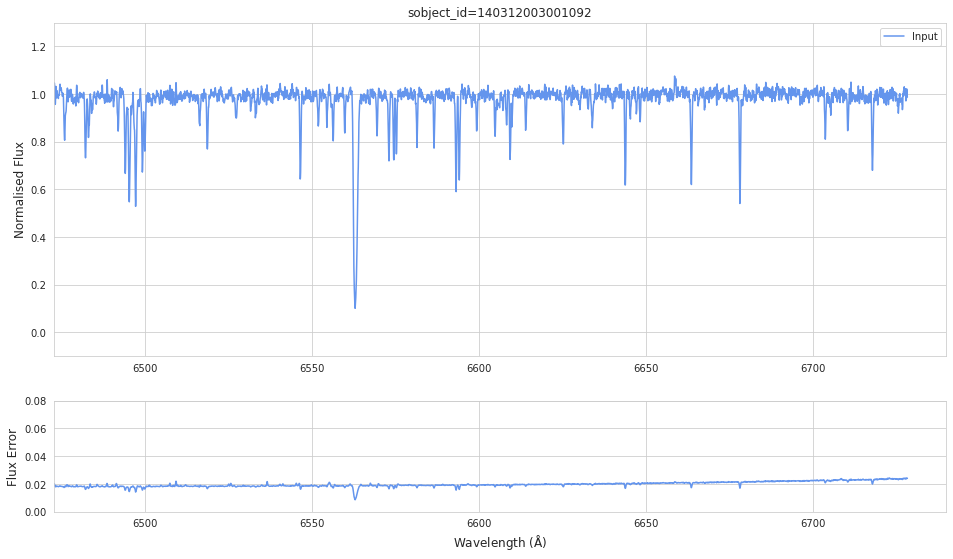
\includegraphics[scale=.40]{figures/input spectrum.png}
\caption{Red camera normalised flux data and error for the \texttt{sobject\_id = 140312003001092}, prior to re-sampling.}
\end{figure}

To significantly minimise over-sampling and under-sampling, the spectra under consideration were interpolated to a common wavelength grid with a sampling rate equivalent to 0.06 \r{A}. This rate is accurate to the sampling rate of each spectrum generated by the red camera to the second decimal place.

\begin{figure}[!htb]
\centering
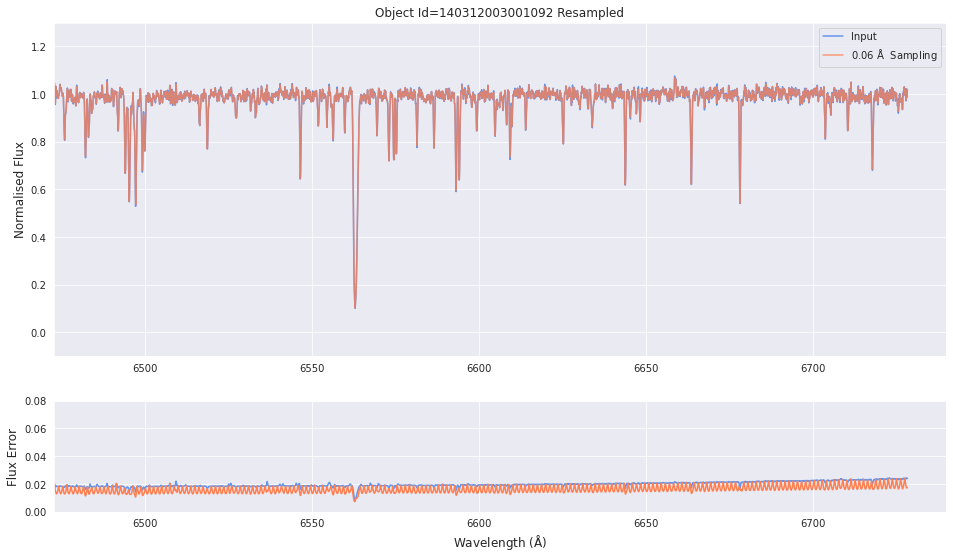
\includegraphics[scale=.40]{figures/resampling example.png}
\caption{\texttt{sobject\_id = 140312003001092}, re-sampled.}
\end{figure}

This work used the \texttt{spectres} Python package \citep{carnall2017spectres} to efficiently sample all red camera spectra to the following common wavelength grid.

\[\lambda_{min} = 6472.5\]
\[\lambda_{max} = 6740\]
\[\Delta\lambda = 0.06\]

This grid was chosen based on the range of wavelength separation observed in the raw data as well as the work of Čotar et al. Normalised spectra and their errors from the red camera were subjected to this process. The authors of DR3 have set the continuum value for the normalised spectra at 1. Thus, spectra for which flux values were not recorded at the tail and top end of the interpolated grid, were padded with the value 1 in order to maintain the uniformity of the common wavelength grid. Re-sampling is computationally intensive and thus this process was offloaded to a university server. The resultant data and interpolated errors were saved as HDF5 files using the \texttt{.h5} file format in a single array for convenience. 

\section{Region Selection}

This work exploited the use of effective spectral region selection to reduce the feature and search space as well the memory and disk footprint. It was demonstrated previously that the total number of spectral features for the red camera is $\sim$ \num[round-precision=2,round-mode=figures, scientific-notation=true]{2928752091}. P Cygni, inverse P Cygni and other emission-line stars considered in this work show characteristic emission and absorption profiles near the H$\upalpha$ line. This observation can be used to significantly reduce the size of the feature space. 

The region of interest around H$\upalpha$ was selected to be 6561\r{A} - 6565\r{A} \citep{traven2017galah}. By repeating the feature space calculation above it can be noted that this region is sufficiently narrow enough to reduce the feature space by a hundredfold to $\sim$ \num[round-precision=2,round-mode=figures, scientific-notation=true]{45228200} while simultaneously ensuring that it can encapsulate the emission features under consideration. 

In code, this selection was implemented as a binary spectral mask which extracts the flux values for the relevant wavelength range while masking flux values outside this range. A masked version of the re-sampled data was stored in a separate \texttt{.h5} file for convenience. In terms of memory and disk allocation, this had the effect of reducing the memory footprint from $\sim$60GB for the re-sampled red camera data to $\sim$1GB for the H$\upalpha$ masked version of the same data. This improved the speed of read/write operations significantly. 

\section{Concluding Remarks}

This work draws the following conclusions from the analysis presented above,

\begin{enumerate}
\item When faced with higher dimensional data, dimensionality reduction and sample size pruning can be effective strategies when seeking to identify and classify atypical emission-line spectra. 

\item Open data sets such as that provided by Čotar et al. can be useful as a prototyping aid to iteratively develop and evaluate machine learning methods given the low volume of data compared to GALAH DR3. 

\item Re-sampling can ensure that all spectra can be compared on the same wavelength grid. This is particularly useful for developing machine learning methods as the consistency of the data can be maintained throughout the process, particularly when comparing morphologies of spectra.  

\item Region selection can significantly reduce the feature space and search space by efficiently limiting it to those only the regions that are of interest for a particular study. 
\end{enumerate}



% DTW
\chapter{Developing a Framework for Classification}

The volume and complexity of large spectroscopic datasets pose a significant challenge for developing methods to identify and classify emission-line stars. As previously explored, these and other constraints indicated that it would not be efficient or an effective use of time to trial multiple machine learning methods in pursuit of the end goals. As a result, a general framework and set of principles was developed based on the background provided in Chapters 1 to 3. These principles guided the development of a viable prototype method upon which the total machine learning method was built. The details of this framework, the methods that were selected, the {\em raison d'être} for these decisions and the results from the prototype are presented in the following sections.

\section{Requirements and Constraints}

As shown in prior chapters, morphological classification based on visual inspection of spectra cannot scale feasibly with the volume of data present in GALAH DR3. And while machine learning methods such as t-SNE and autoencoders \citep{traven2017galah, vcotar2021galah} have been relatively successful in detecting H$\alpha$ emission spectra, neither technique is able to further classify emission-line spectra into classes, such as P Cygni and inverse P Cygni.

When developing a framework for classification, it was found that an approach that is sensitive to the meaningful morphological differences between P Cygni, inverse P Cygni and other species is an important requirement. Given that the feature space is of size $\sim$ \num[round-precision=2,round-mode=figures, scientific-notation=true]{2928752091}, a classification method must be able to overcome the "curse of dimensionality" and be computationally and memory efficient. Feature engineering must capture the understanding that P Cygni spectra exhibit a redshifted emission peak, while the inverse P Cygni spectra exhibit a blueshifted peak. A method should also be able to differentiate between classes such as double-peaked emission spectra and emission lines superimposed on absorption. This can be quite intuitive for a human being to do manually, but can prove challenging for a machine, as it must be trained on a well-constructed training data set that is sensitive to these features. 

Given that DR3 does not have labeled samples of P Cygni and inverse P Cygni spectra, a supervised learning approach to classification was not suitable. This narrowed the approach to the unsupervised learning domain. Chapter 2 demonstrated that well-known unsupervised clustering methods such as k-means clustering generally fail to cluster and classify emission-line spectra \citep{garcia2018machine}. Given this result, this and related methods were not given further consideration. Instead, a first principles-based approach was adopted, with a focus on methods that are sensitive to morphological similarities and differences between spectra. More rudimentary methods, such as cross-correlation of signals, are examples of methods that could be sensitive to the various emission line morphologies. However, given that a labeled data set of the various classes of emission-line spectra in DR3 did not exist, this line of inquiry was abandoned as it was not possible to create mean spectra for convolving against all DR3 spectra for the various potential classes. Instead, methods were explored that created effects similar to pairwise cross correlation, provided a similarity score (or equivalent) with limited human intervention, and had minimum reliance on rule-based approaches that have been used in the past, for instance, \citep{traven2015gaia}. 

These constraints narrowed the search for suitable methods to a field known as unsupervised time series clustering, more specifically a clustering method based on a concept used extensively in signal processing called dynamic time warping (DTW) \citep{kruskal1983overview}. First introduced in 1975 as an algorithm for speech recognition \citep{itakura1975minimum}, DTW has been modified and adapted extensively in various scientific disciplines such as signal processing, telecommunications and biomedical engineering. It was demonstrated in Chapter 2 that DR3 spectra, and indeed all spectra, are mathematically analogous to time series; while an individual spectrum does not contain a time axis, the monotonically-increasing wavelength grid serves as the analogue of the time axis. Time series methods such as DTW have been more generally developed in the domain of time series analysis \citep{nielsen2019practical} and can be suitably adapted to stellar spectra. With clustering, this work did not rely on labelled data, but rather took a data-driven approach that learns from the emission-line morphologies present in the normalised spectral data present in DR3.

\section{Dynamic Time Warping}

Dynamic time warping (DTW) is a time series analysis algorithm that can measure similarity between two temporal sequences. The similarity can then be used to cluster morphologically similar spectra into meaningful groups. These clusters can then be used to classify spectra into distinct classes. 

DTW is suitable for clustering problems where the morphology of the signal plays a salient role over other features \citep{nielsen2019practical} and where labeled data are unavailable. The name is inspired by the method itself, in which two signals are stretched or warped to align them on the temporal axis. For stellar spectra, this warping takes place in the wavelength domain and thus produces a discrete dynamic {\em wavelength} warping effect.

\begin{figure}[!htb]
\centering
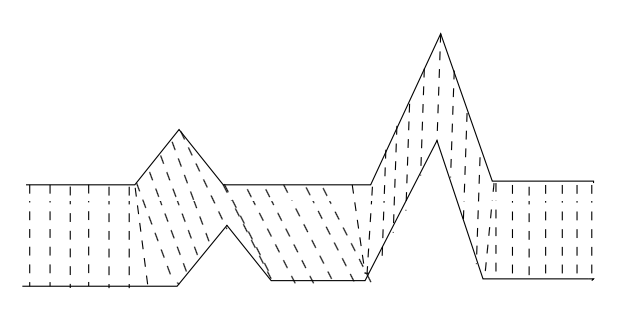
\includegraphics[scale=1]{figures/Dynamic_time_warping.png}
\caption{Each point on the wavelength grid is mapped to a point on the opposite spectrum, but there is no requirement that the mapping is one to one. Reproduced from \citet{nielsen2019practical}}
\label{fig4.1}
\end{figure}

As indicated in Figure \ref{fig4.1}, the algorithm works by expanding or contracting the wavelength axis to find the best alignment and thus ensuring that morphologically similar spectra can be compared. This algorithm is often described as being similar to comparing the shape of signals visually. The algorithm follows several steps and has several constraints which are as follows:

\begin{enumerate}
    \item Every point on the spectrum must be matched with at least one point of the other spectrum.
    \item The first and last indices of each spectrum must be matched with their counterparts in the other spectrum.
    \item The mapping must be such that the wavelength is increasing rather than decreasing, i.e. the method should not match a point on one spectrum to a point on the other spectrum that has passed. 
\end{enumerate}

Steps 2 and 3 do not have a significant impact on the dataset being used in this work as the data are sampled to the same wavelength grid and the spectra are thus of equal length. 
There are many possible ways to align two spectra while adhering to these constraints. The algorithm chooses the alignment that minimises the distance between the spectra. This distance is a cost function and is measured as the sum of the absolute differences between matched points. The absolute difference in this context is the difference between the points' values (wavelength values). This distance measure then serves as the basis for clustering.


The Pythonic representation of this algorithm is as follows:

\begin{lstlisting}[language=Python]
# Primary function
def distDTW(lambda1, lambda2):
     DTW={}
     for i in range(len(lambda1)):
         DTW[(i, -1)] = np.inf
     for i in range(len(lambda2)):
         DTW[(-1, i)] = np.inf
     DTW[(-1, -1)] = 0
 
# Calculate the optimum i.e. where distance is minimum
     for i in range(len(lambda1)):
         for j in range(len(lambda2)):
             dist = (lambda1[i] - lambda2[j])**2
             DTW[(i, j)] = dist + min(DTW[(i-1, j)],
                                      DTW[(i, j-1)], 
                                      DTW[(i-1, j-1)])
 
 # Return the associated distance between two spectra
     return sqrt(DTW[len(lambda1)-1, len(lambda2)-1])
\end{lstlisting}

Despite the effectiveness of this algorithm, the computational complexity is still of order $O(N^2)$. As this presents a significant computational cost and overhead, the method developed here relies on a linear time complexity approximation—i.e., the $O(N)$ Python language implementation of DTW called \texttt{FastDTW}—to compute the optimum distance between spectra and thus the similarity \citep{salvador2007toward}. %\texttt{FastDTW} is a linear approximation to the DTW method above. 
A full discussion of how \texttt{FastDTW} compares to other implementations of DTW is beyond the scope of this thesis.

In addition to computational complexity, an important consideration is available memory. Generally, all spectral data must be loaded into memory (RAM) when computing DTW distances. In the case of DR3, this implies holding $\sim$ \num[round-precision=2,round-mode=figures, scientific-notation=true]{2928752091} features in memory. The computational hardware available for this project had a memory capacity of $\sim$ 300 GB. \texttt{FastDTW} in particular required a memory capacity of at least 1TB for the $\sim$ \num[round-precision=2,round-mode=figures, scientific-notation=true]{2928752091} features. This is a significant amount of data to hold in memory and presented a serious obstacle.

Two strategies were developed to overcome these challenges and reduce computational and memory overheads. These are as follows:

\begin{enumerate}
    \item Reduce the number of features. As explained in a Chapter 2, only the region around H$\alpha$ is pre-selected in this work, and \texttt{FastDTW} was run only on this region.
    \item Reduce the search space from the entire DR3 data set to a subset which has a higher chance of yielding P Cygni, inverse P Cygni and other emission-line spectra. The existence of H$\alpha$ emission-line spectra is effectively a precursor to the existence of P Cygni and inverse P Cygni spectra. Thus the H$\alpha$ emission-line data set from \citet{vcotar2021galah} was used for prototyping this method. This subset with $\sim$ 10,000 spectra includes data from GALAH and other related surveys with the HERMES spectrograph. It is assumed that this data set only contains H$\alpha$ emission-line spectra, although  \citet{vcotar2021galah} have indicated that this data set  could contain non-emission-line (``typical'') spectra as well, albeit as a comparatively minor proportion. 
\end{enumerate}

There are many machine learning methods that can be used to cluster groups of similar and dissimilar observations. These methods will generally compute method-specific distance measures as a similarity metric. DBSCAN, for example, computes a method-specific distance which cannot be overridden by a pre-computed distance metric such as a DTW distance \citep{traven2017galah}. It is unclear whether a DBSCAN distance metric, or indeed a distance metric other than DTW, can capture the morphological features of emission-line stars. Due to time constraints, a thorough evaluation of the alternative distance metrics provided by the various clustering methods available was not undertaken. Instead, a clustering method which can accommodate pre-computed distances was chosen: agglomerative hierarchical clustering. 

\section{Agglomerative Hierarchical Clustering}

Agglomerative hierarchical clustering is a method that can take a pre-computed distance metric such as a DTW distance, and use it to cluster observations into classes. It is a well-understood and robust method that has proven to work well on time series problems relying on DTW distances \citep{nielsen2019practical}.

With a similarity measure such as the pairwise DTW distances between spectra, hierarchical clustering can be used to group similar spectra into similar clusters. Once a similarity measure (or a dissimilarity measure) has been specified, hierarchical clustering produces a representation in which clusters at each level of the hierarchy are created by merging clusters at the next lower level. At the lowest level, each cluster contains a single observation. At the highest level, there exists a single cluster that contains all of the data \citep{hastie2009elements}. There are two basic paradigms to traverse these levels (or tree), namely, aggolomerative (bottom-up) and divisive (top-down). 

With agglomerative clustering, each spectrum will initially form a singleton cluster. At each step, the most similar spectra will be merged into a single cluster, producing one less cluster at the next higher level. The similarity between two spectra is based on the pre-computed DTW distance between them. A lower distance implies a greater similarity, while a higher distance indicates a dissimilarity.  

Based on the similarity (and dissimilarity) between individual spectra, a cluster dissimilarity can also be defined. Consider two clusters called $A$ and $B$. The dissimilarity between the two clusters $d(A,B)$ is computed from the set of pairwise dissimilarities $d_{ij}$, where one member of the pair, $i$, is in $A$ and the other, $j$, is in $B$. The complete linkage dissimilarity between the two clusters is set to be the dissimilarity of the furthest (most dissimilar) pair of spectra,
\begin{equation}
    d(A,B) = \max_{\substack{i \in A \\ j \in B}} d_{ij}
\end{equation}

This is also known as the farthest neighbour method. Other dissimilarity measures such as single linkage dissimilarity or nearest neighbour dissimilarity can be defined as
\begin{equation}
    d(A,B) = \min_{\substack{i \in A \\ j \in B}} d_{ij}
\end{equation}

Hierarchical clusters can be visualised using a dendogram. A dendogram is a binary tree that represents the recursive agglomeration (or division) of clusters. The height of the tree (or a branch) is proportional to the inter-group dissimilarity defined above. 

\begin{figure}[!htb]
\centering
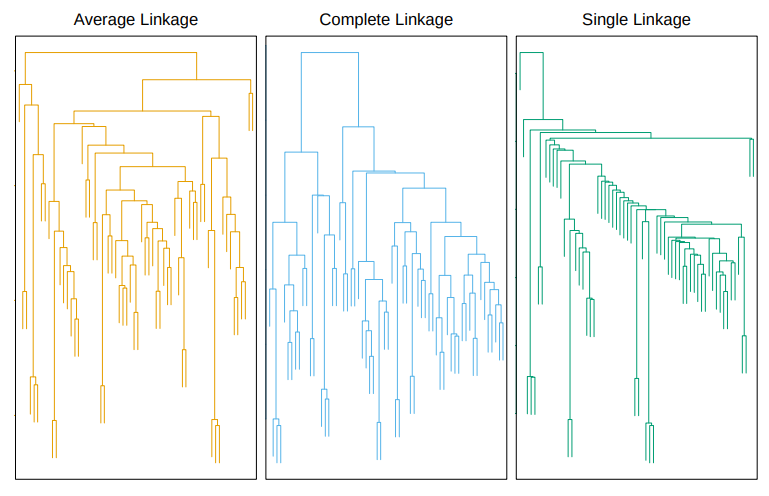
\includegraphics[scale=0.60]{figures/complete linkage.png}
\caption{Dendograms for a given toy data set using different similarity measures. Note the longer branch lengths of the complete linked tree that selects for maximum dissimilarity. Reproduced from \citet{hastie2009elements}.}
\end{figure}

This work used the complete linkage dissimilarity to cluster spectral groups. The justification for using this measure over the single linkage dissimilarity is to force the separation of P Cygni and inverse P Cygni spectra into distinct groups by exploiting the maximum distance between two individual spectra that belong to these groups. Other distance measures such as group average clustering use the average dissimilarity between groups. Group average clustering can be less accurate in separating the data into clusters as it relies on an average spectrum per cluster, which may not completely capture the variation of spectral morphologies within a cluster. Therefore this measure was not considered, as it may be less accurate in separating P Cygni from inverse P Cygni and other emission-line spectra due to this averaging or smoothing effect. This work also relies on the agglomerative (bottom-up) method, as it is more robust and has been studied extensively in the literature compared to the divisive (top-down) method \citep{hastie2009elements}.

\subsection{Selecting the Number of Clusters}

Given that the framework proposed above is an entirely unsupervised machine learning approach, it is generally not required that the number of clusters be specified in advance. In the absence of a predefined value for this parameter, the typical approach would require a plot of the dendogram where suitable cuts can be made at a required level. However, since the tree can theoretically be cut at any level, and can have a maximum number of clusters equal to the number of samples and a minimum number of clusters equal to 1, a more meaningful and reliable cut can be made with the aide of astrophysical domain knowledge, as will be demonstrated below. In the absence of such knowledge, this work would have to cut the dendogram at each level, examine the clusters and subsequently decide on a suitable number of clusters. Furthermore, given that the sample size is at least 10,000 spectra, visually inspecting a dendogram for this data set can be challenging. Where possible, this work used prior art such as \citet{reipurth1996halpha}, \citet{traven2017galah}, and \citet{zhang2021catalog} to determine the number of clusters, thus eliminating the requirement to visually inspect a complex dendogram of the order of thousands of branches. 

Classes of H$\alpha$ emission-line spectra have been found using manual methods and as such, prior work can provide some guidance regarding the number of clusters. \citet{reipurth1996halpha}, in particular, proposed the existence of seven morphological groups which include P Cygni and inverse P Cygni, as well as five other H$\alpha$ emission-line classes. However, if the number of clusters is set to a value of two, there is a significant risk that other morphologies will be included in the P Cygni cluster and inverse P Cygni cluster, thus leading to erroneously classified/labelled clusters. Thus, based on the prior art, this work took the number of clusters to be between six and ten as a suitable range. The number of samples were significantly higher than any data sets in prior art, especially the manual classification approaches detailed in the prior chapters. The justification to use a higher number of clusters such as ten is to account for the possibility of additional morphological classes that may have been missed in the prior art during manual classification. As it will be demonstrated in Chapter 6, this over-classification can be beneficial when working with more complex data sets.

\section{Results}

The results of the DTW distance calculation can be visualised as a distance cost plot. Figure \ref{fig4.3} includes the pairwise distances for 6,977 samples from DR3 that are present in the \citeauthor{vcotar2021galah} data set after the application of DTW. Note that the plot resembles a triangular matrix with the diagonal representing a value of zero for the self distance of a spectrum. Lower values indicate higher similarity while higher distance values indicate lower similarity (or greater dissimilarity). Zooming into a region reveals further structure concerning similar and dissimilar spectra. The zero distance diagonal and the triangular nature of the distance matrix, are visible on this plot.

\begin{figure}[!htb]
\centering
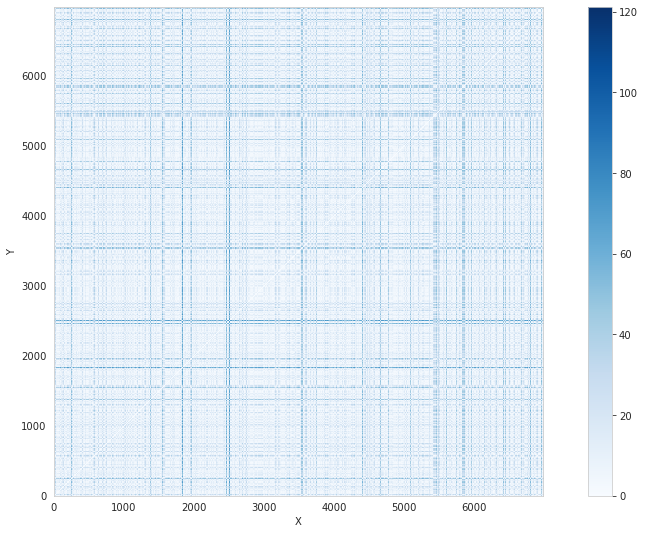
\includegraphics[scale=0.60]{figures/dtw cotar.png}
\caption{Pairwise DTW distances for spectral samples in \citet{vcotar2021galah}.}
\label{fig4.3}
\end{figure}

This distance matrix was used as the basis for complete linkage aggolomerative hierarchical clustering. The number of clusters was varied between seven and ten. A mean silhouette score was calculated for each selection. This score was used as an additional selection criterion for the number of clusters. Silhouette scores can range between -1 and 1. Negative scores indicate that samples may be assigned to the wrong cluster. Values extremely close to zero indicate that clusters may overlap. The best achievable value is 1, although this is rare in practical unsupervised clustering problems. Thus the silhouette score is a measure of the efficacy of the clustering process.

\begin{figure}[!htb]
\centering
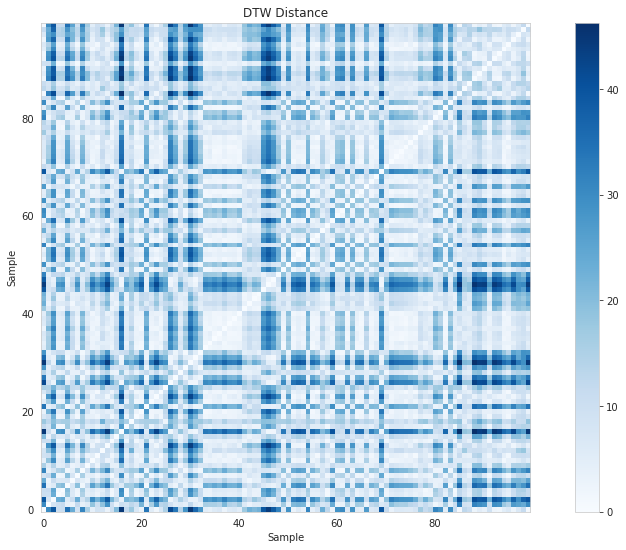
\includegraphics[scale=0.60]{figures/dtw cotar zoomed.png}
\caption{Pairwise DTW distances for spectral samples in \citet{vcotar2021galah} (zoomed).}
\end{figure}

In order to calculate the mean silhouette score, silhouette coefficients for all samples must be calculated as follows:

Compute the mean within-cluster distances given by $a$ and then compute the mean nearest-cluster distance $b$ for each sample. The sample silhouette coefficient is then given by

\begin{equation}
\frac{(b-a)}{\max_{}(a,b)}
\end{equation}

Once the coefficient for each sample was calculated, the mean silhouette score for the entire sample was computed. Table \ref{table:Silhouette Score} summarises the scores obtained.

\begin{table}[]
\begin{center}
\begin{tabular}{|c|c|}
\hline
\textbf{Number of Clusters} & \textbf{Silhouette Score} \\ \hline
6                     & 0.2904                    \\ \hline
7                     & 0.3033                    \\ \hline
8                     & 0.3005                    \\ \hline
9                     & 0.3092                    \\ \hline
10                    & 0.3044                    \\ \hline
\end{tabular}
\caption{Silhouette score comparison}
\label{table:Silhouette Score}
\end{center}
\end{table}

At face value it appears that nine clusters is the optimum, given that this produces the largest silhouette score. However, upon closer examination it was concluded that ten was more suitable under the essential constraint that P Cygni and inverse P Cygni spectra should be adequately separated from other clusters. Thus, the spectra that belong to each cluster for both nine clusters and ten clusters were plotted. For nine clusters, while a P Cygni only cluster was identified, a cluster containing only inverse P Cygni spectra was not identified. However, when this parameter was set to ten, two clear clusters of P Cygni and inverse P Cygni spectra were identified.

\begin{figure}[!htb]
\centering
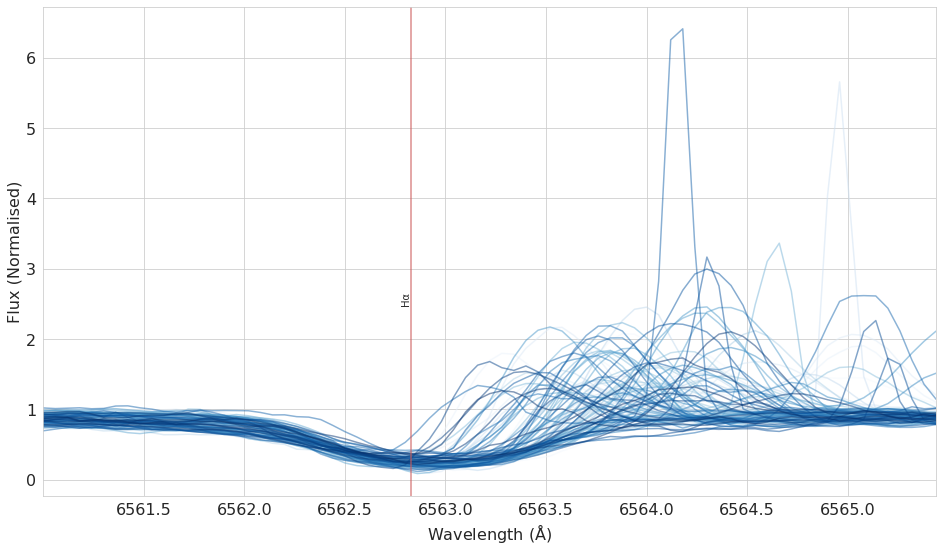
\includegraphics[scale=0.45]{figures/pcygni.png}
\caption{102 P Cygni spectra identified using clustering.}
\end{figure}

\begin{figure}[!htb]
\centering
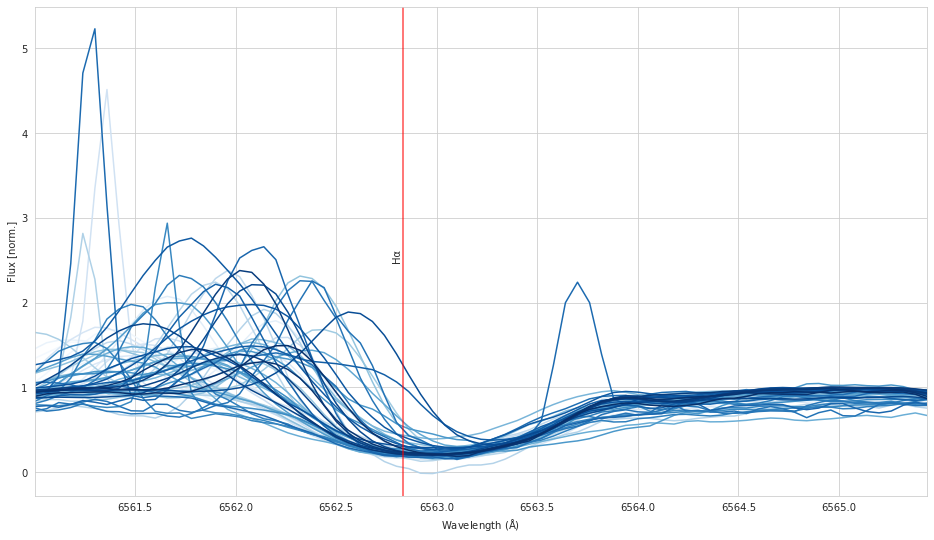
\includegraphics[scale=0.45]{figures/inverse p cygni.png}
\caption{62 Inverse P Cygni spectra identified using clustering.}
\label{fig4.6}
\end{figure}

Eight other clusters with various emission-line morphologies, such as double peak emission, were also identified. Other classes are presented in the Appendix. Given the silhouette score, it is possible that some P Cygni and inverse P Cygni spectra may have been mis-classified (see Figure \ref{fig4.6}) and included in other classes. This can be addressed by further sub-clustering and classifying spectra via a second pass of the scheme above. This work, however, did not progress with multiple passes of this method due to time constraints. 

A sub-classification of the P Cygni and inverse P Cygni classes discovered in this process is presented in Chapter 5, where these results are compared to t-SNE. The advantages and disadvantages of this approach compared to t-SNE are also discussed in that chapter. 

\section{Line Fitting}

The P Cygni and inverse P Cygni spectra thus classified were modeled using a double Gaussian, with an offset for one of the Gaussian functions \citep{traven2015gaia, zhang2021catalog}. This mixture model with two Gaussians can be used to fit the line profile of P Cygni and inverse P Cygni spectra. Given that there are 102 P Cygni spectra that require fitting, this work adopted a semi-automated method where the initial conditions for the model parameters were driven by the data. Notably the minimum and maximum local flux values were used to set both the amplitude and mid-value of each peak and trough.

This work then utilised the popular Python based numerical optimisation package, \texttt{scipy} \citep{2020SciPy-NMeth} to generate fitted models for the P Cygni and inverse P Cygni spectra using least squares optimisation.

The Gaussian mixture model is defined as, 

\begin{equation}
    f(x) = \frac{A}{\sigma_1\sqrt{2\pi}} 
  \exp\left( -\frac{1}{2}\left(\frac{x-\mu_1}{\sigma_1}\right)^{\!2}\,\right) + \frac{B}{\sigma_2\sqrt{2\pi}} 
  \exp\left( -\frac{1}{2}\left(\frac{x-\mu_2}{\sigma_2}\right)^{\!2}\,\right) + C
\end{equation}


This seven parameter model contains an offset parameter $C$ to account for the inverted Gaussian required to model the absorption trough/line of the P Cygni and inverse P Cygni spectra. The parameters A and B are to account for the respective amplitudes of the emission and absorption lines. The uncertainties of this fit can be modelled more accurately within a Bayesian framework and the use of MCMC estimation \citep{hogg2010data}. A detailed discussion of this framework and estimation method is, however, beyond the scope of this work.

\begin{figure}[!htb]
\centering
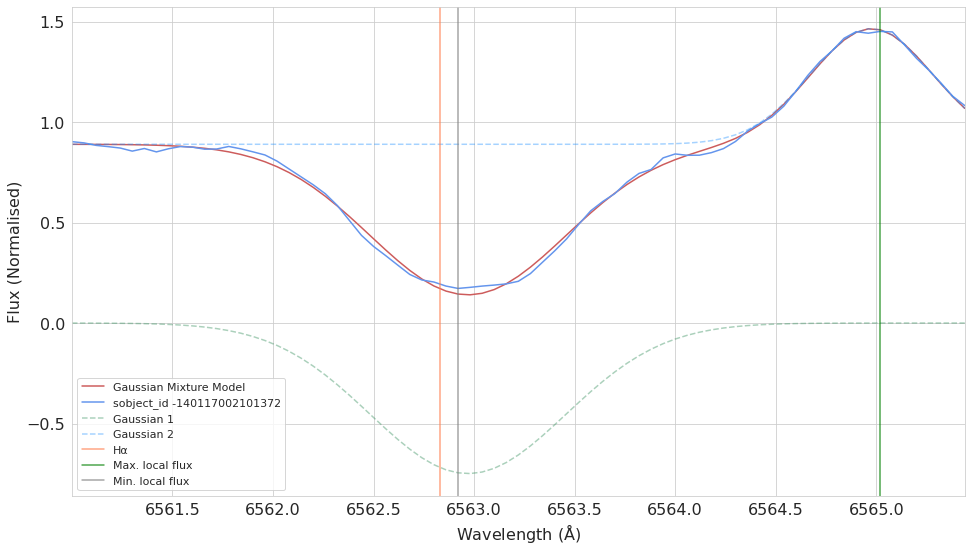
\includegraphics[scale=0.45]{figures/p cugni fitted.png}
\caption{A Gaussian mixture model fit of one of the identified P Cygni spectra.}
\end{figure}

The line-fitting method described can be repeated for each P Cygni spectrum discovered by clustering. Presented below are a few examples of these fitted models. This technique can also extended to the inverse P Cygni spectra.

\begin{figure}[!htb]
\centering
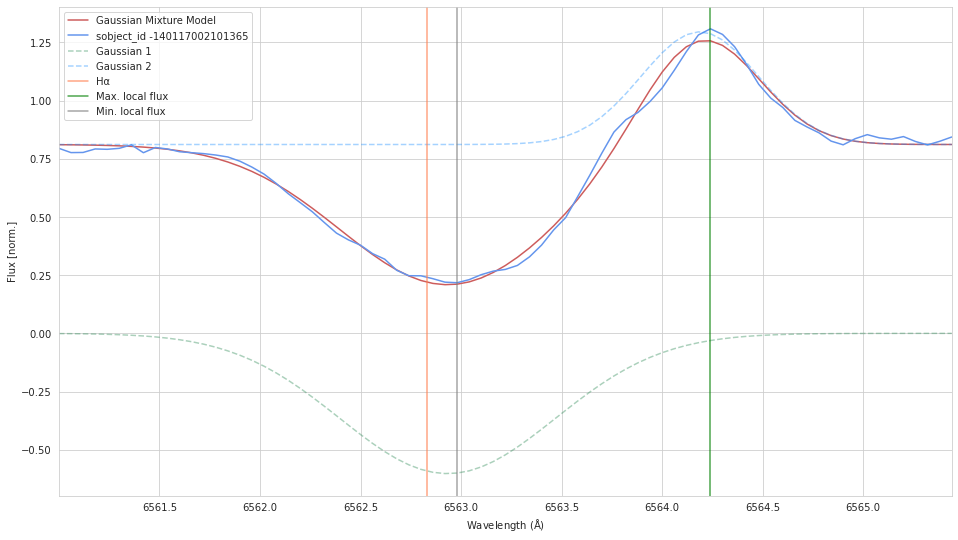
\includegraphics[scale=0.45]{figures/p cygni fitted 2.png}
\caption{A Gaussian mixture model fit for sobject ID 140117002101365. }
\end{figure}

\begin{figure}[!htb]
\centering
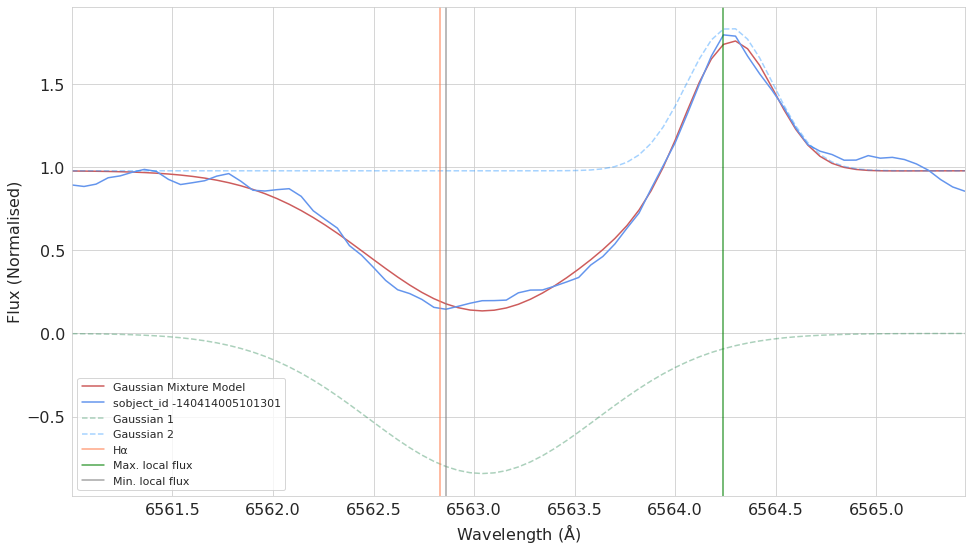
\includegraphics[scale=0.45]{figures/p cygni fitted 3.png}
\caption{A Gaussian mixture model fit for sobject ID 140414005101301. }
\end{figure}

\begin{figure}[!htb]
\centering
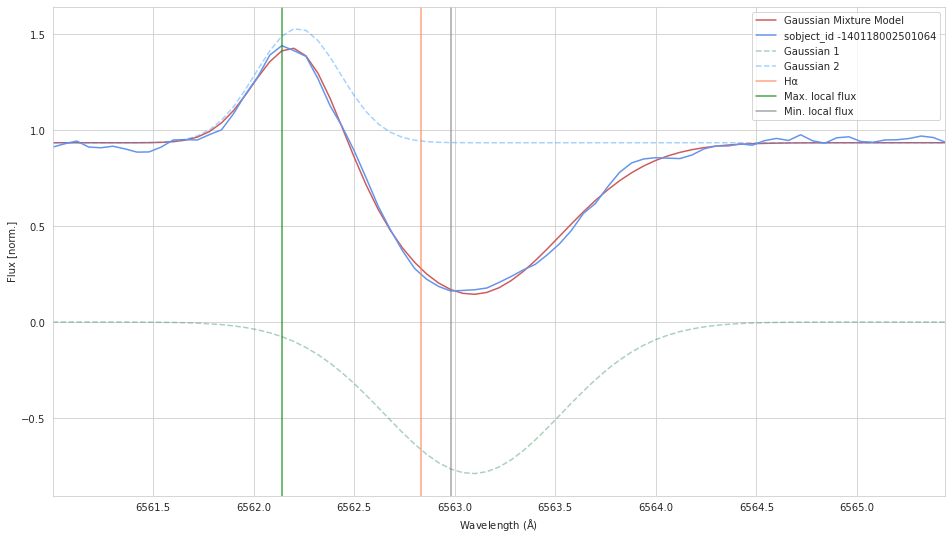
\includegraphics[scale=0.45]{figures/inverse p cygni 1.png}
\caption{A Gaussian mixture model fit of one of the identified inverse P Cygni spectrum. }
\end{figure}

\begin{figure}[!htb]
\centering
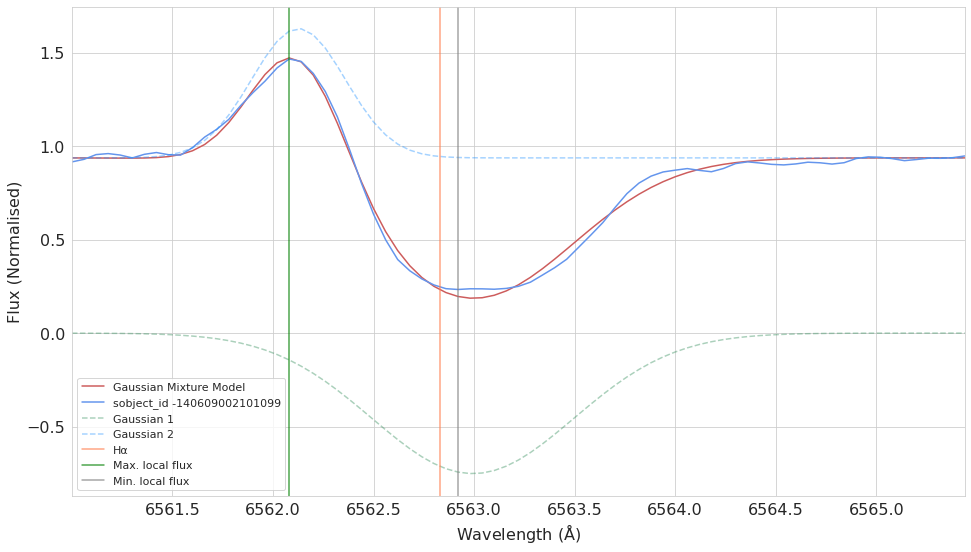
\includegraphics[scale=0.45]{figures/inverse p cygni fitted 2.png}
\caption{A Gaussian mixture model fit for one of the identified inverse P Cygni spectrum.}
\end{figure}

\section{Concluding Remarks}

Once a framework was developed, the sample data provided by \citet{vcotar2021galah} significantly accelerated the development of the methods discussed above. The primary reason for this is that methods can be tested and iterated at a more rapid pace given that the sample size was significantly smaller than GALAH DR3. Additionally, the sample data was well-pruned and presumably only consisted of emission-line spectra, although this sample purity may not be guaranteed. These conclusions make a strong case for the availability of open access data and code.

Dynamic time warping was able to learn from the data presented and provide pairwise distances that can capture the morphologies of the spectra. Combined with agglomerative hierarchical clustering, DTW can form the basis of a machine learning method that can identify, cluster and classify P Cygni, inverse P Cygni and other types of emission-line spectra.

Compared to methods such as k-means, logistic regression and t-SNE presented in Chapter 2, it can be argued that DTW is more sensitive to the morphological differences and similarities between spectra. In Chapter 2, t-SNE was also introduced as a method to identify H$\alpha$ emission-line spectra in GALAH. Given the efficacy of DTW on a set of emission-line spectra provided by \citet{vcotar2021galah}, this work considered whether t-SNE can be used as a pre-processing step in identifying emission-line stars prior to applying DTW. This hypothesis was tested, and the results are presented in the next chapter. 










% tSNE
\chapter{Evaluation of t-SNE for H$\alpha$ Emission Candidate Selection}

\section{Introduction to t-SNE}

t-distributed stochastic neighbour embedding, or t-SNE is a dimensionality reduction technique \cite{van2008visualizing} that can be used to map higher dimensional data to a two dimensional plane. This t-SNE map can the be used to cluster and classify similar data points into groups and classes using clustering techniques such as DBSCAN. Often, similar objects will be in close proximity to each other in the lower dimensional space. However, this is not guaranteed. In particular, this similarity measure may not be sensitive to morphological differences in the spectra. Thus, the use of t-SNE must be carefully evaluated if it is to be used as an H$\alpha$ emission candidate selection subroutine as proposed by work such as Traven et al. \cite{traven2017galah}.

Thus DR3 spectra of high dimensionality, can be mapped to a two dimensional representation in order to overcome the curse of dimensionality. If it can be assumed that relevant features in the higher dimensional representation that are common to H$\alpha$ emission candidates are preserved during the mapping from higher dimensions to two dimensions, then this fact can be used to segment H$\alpha$ emission candidates into a distinct class. This class can then be used as a starting point for further analysis using the DTW pipeline demonstrated in chapter 4. 

t-SNE has been used successfully in the past to separate and segment a subset of H$\alpha$ emission candidates in the GALAH survey \cite{traven2017galah}. This study isolated 215 H$\alpha$ and H$\beta$ candidates from a prior GALAH data release of approximately 300,000 spectra. 

However, the preservation of features from high dimensions to two dimensions such that H$\alpha$ emission candidates can be meaningfully separated from normal or average spectra is not guaranteed. The pipeline for P Cygni and inverse P Cygni detection presented in chapter 4 relies on a meaningful and confident selection of H$\alpha$ emission candidates from the GALAH survey prior to the application of DTW and clustering. In subsequent sections, this chapter will demonstrate that t-SNE may not be a sufficiently robust technique to serve as the H$\alpha$ emission candidate selection step that is critical for the DTW based framework presented in chapter 4.

\subsection{Mathematical foundations of t-SNE}

This section presents a brief mathematical introduction to t-SNE adapted from Traven et al. \cite{traven2017galah}. A more detailed discussion is found in Van der Maaten and Hinton \cite{van2008visualizing}. 

Consider $N$ spectra where each spectrum is a higher dimensional object $x_i$. The low dimensional representation of this data is achieved by the optimal positioning of data points in the lower dimensional projection map. In order to achieve this, the t-SNE process defines a similarity between data points in the original higher dimensional space $X$ and in the lower dimensional project space, (2-dimensional for the purpose of this work) $Y$. These are described by the symmetric joint-
probability distributions $P$ and $Q$, respectively

The pairwise similarity between data points $x_i$ and $x_j$ is modeled by the probability that one data point would pick another data point as it's neighbour. This depends on the probability density under a Gaussian in space $X$ while a Student's t-distribution is used in space $Y$. t-SNE first computes probabilities $p_{ij}$ that are proportional to the similarity of spectra $x_i$ and $x_j$ as follows,


For $i$ $\neq$ $j$,

\begin{equation}
p_{j\mid i}={\frac {\exp(-\lVert \mathbf {x} _{i}-\mathbf {x} _{j}\rVert ^{2}/2\sigma _{i}^{2})}{\sum _{k\neq i}\exp(-\lVert \mathbf {x} _{i}-\mathbf {x} _{k}\rVert ^{2}/2\sigma _{i}^{2})}}
\end{equation}

Note that $p_{i\mid i}=0$ and $\sum _{j}p_{j\mid i}=1$ for all $i$. Now define,

\begin{equation}
    p_{ij}={\frac {p_{j\mid i}+p_{i\mid j}}{2N}}
\end{equation}

and note that $p_i_j=p_j_i$, $p_i_i=0$ and $\sum _{ij} p_i_j=1$

The bandwidth of the Gaussian distribution $\sigma_i$ is set such that the perplexity of the conditional distribution equals a predefined perplexity. This perplexity is a user defined quantity and is considered a hyper-parameter of this method. This implies that the bandwidth is adapted to the density of the data, Smaller values of $\sigma_i$ are thus used in denser parts of the data space $X$. 

Next, t-SNE will attempt to learn a lower dimensional map with objects $y_i$ in $Y$ that reflect the similarities $p_i_j$ computed above as well as possible. The process measures similarities $q_i_j$ between two points $y_i$ and $y_j$ using a similar approach. 

For $i$ $\neq$ $j$,

\begin{equation}
    q_{ij}={\frac {(1+\lVert \mathbf {y} _{i}-\mathbf {y} _{j}\rVert ^{2})^{-1}}{\sum _{k}\sum _{l\neq k}(1+\lVert \mathbf {y} _{k}-\mathbf {y} _{l}\rVert ^{2})^{-1}}}
\end{equation}

Here $q_i_i=0$ and the t-distribution with one degree of freedom is used to measure similarities between the lower dimensional points. Thus, dissimilar objects will be projected further apart on the map $Y$.

In order to determine the locations $y_i$ on the map $Y$, the non symmetric Kullback–Leibler divergence shown below is minimized using gradient descent. The result of this optimization scheme is a lower dimensional map of the spectral data.

\begin{equation}
    \mathrm {KL} \left(P\parallel Q\right)=\sum _{i\neq j}p_{ij}\log {\frac {p_{ij}}{q_{ij}}}
\end{equation}

This research uses the t-SNE implementation from the popular Python package \texttt{scikit-learn} to generate all t-SNE mappings and results. While other implementations such as multi-core t-SNE exist \cite{Ulyanov2016}, the performance gains of using processor optimised versions of t-SNE over the \texttt{scikit-learn} implementation are modest in this context.

\section{Application of t-SNE to classify H$\alpha$ emission candidates}

This research used an identical approach to Traven et al. on DR3 data to attempt to isolate, cluster and classify potential H$\alpha$ candidates. Such candidates can then be subjected to the pipeline proposed in chapter 4. The first step of this approach involves using t-SNE to dimensionally reduce spectra to a 2-dimensional t-SNE map. The spectra were masked to select the H$\alpha$ region only \cite{traven2017galah}. The perplexity parameter was set to 30 as this provided reasonable separation of classes in Traven et al.

\begin{figure}[h]
\centering
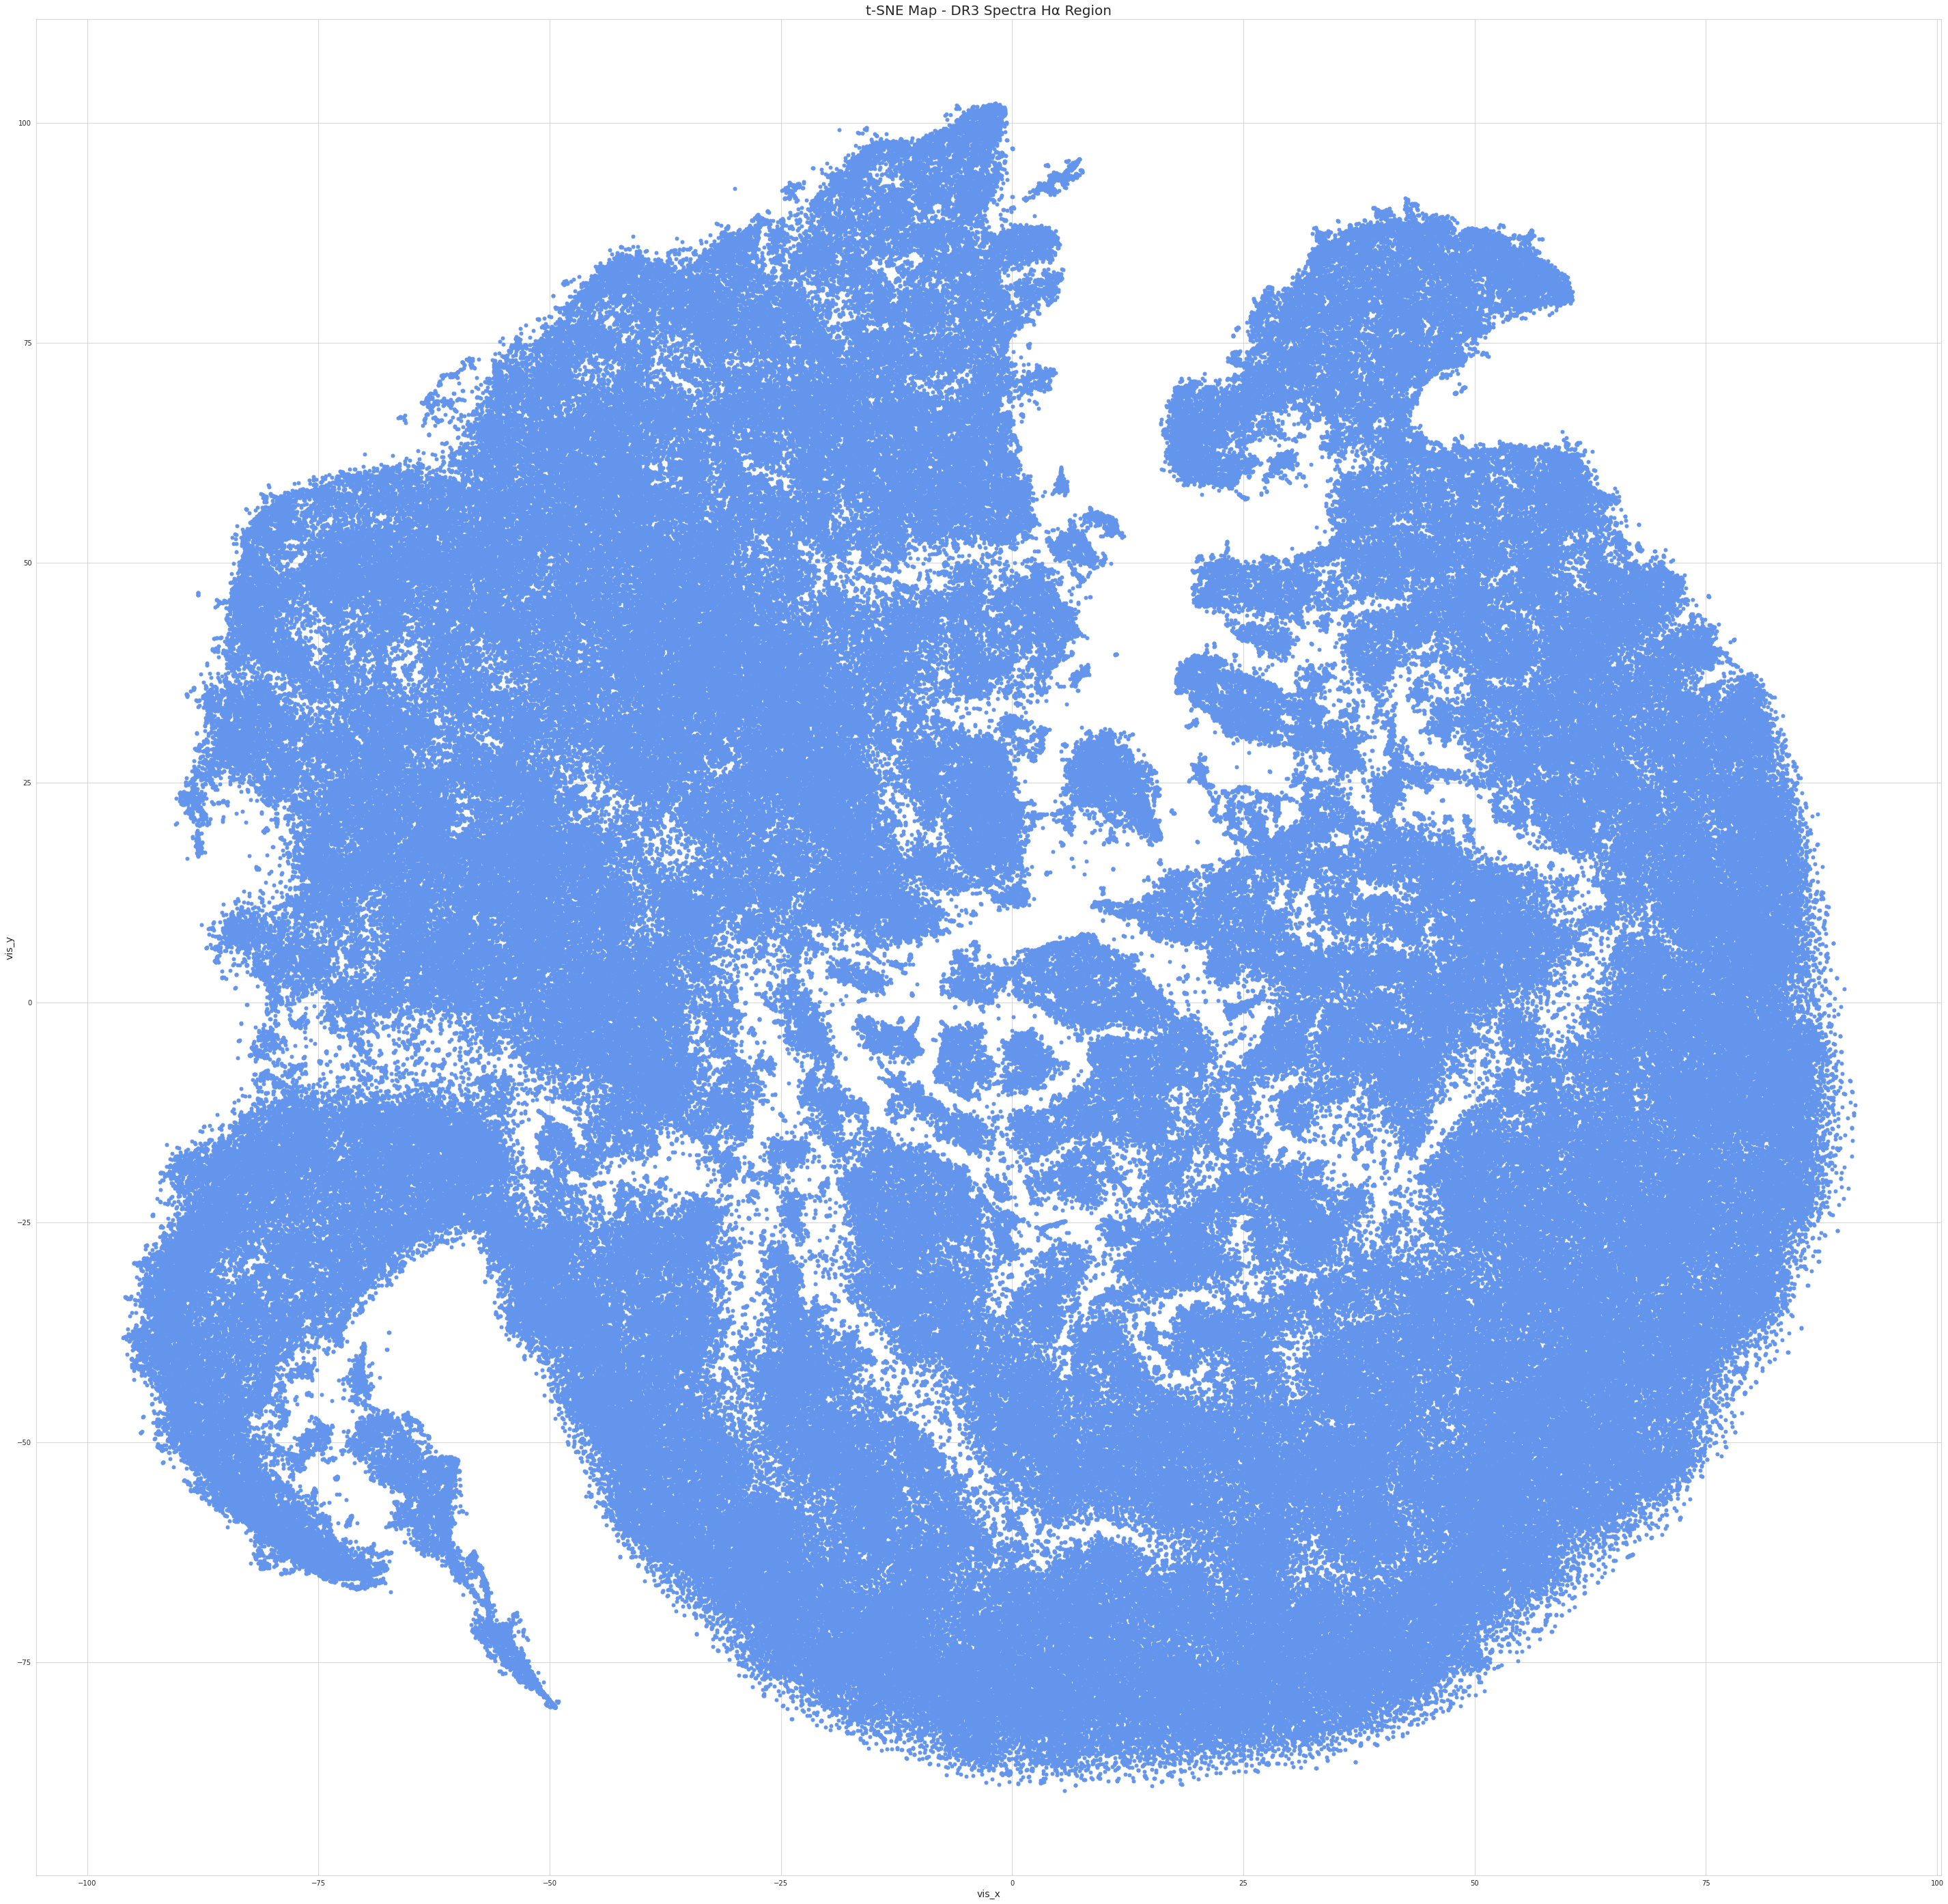
\includegraphics[scale=0.12]{figures/t-sne halpha masked.png}
\caption{t-SNE map for all spectra in DR3. Each point is a 2-dimensional representation of a spectrum. Note that only the region around H$\alpha$ of each spectrum was used to generate this map. The $x$ and $y$ axes contain physically meaningless quantities.}
\end{figure}

\begin{figure}[t]
\centering
\includegraphics[scale=0.12]{figures/t-sne halpha masked with cotar.png}
\caption{t-SNE map for all spectra in DR3 with H$\alpha$ candidates identified by Čotar et al. tagged in pink.}
\end{figure}

In order to validate if the t-SNE plot can adequately separate H$\alpha$ candidates, the validated H$\alpha$ candidates discovered by Čotar et al. \cite{vcotar2021galah} were marked on the same map by using the object IDs. These 7786 spectra are marked in pink in figure 5.2. While a portion of these candidates are clustered in the bottom left quadrant of the map, the other spectra remain scattered across the map with no obvious meaningful cluster that can be separated out of the t-SNE map. 

The current research followed the distance based clustering method used by Traven et al. but could not meaningfully separate the 7786 H$\alpha$ identified by Čotar et al. using this method. Further details of this process and results are provided in the appendix.

\section{Application of t-SNE to classify P Cygni and inverse P Cygni spectra}

The conclusion that can be drawn from the results in section 5.2 is that H$\alpha$ canididates of the order of thousands of spectra cannot be meaningfully separated by the application of clustering methods on the t-SNE plot generated by the method outlined in Traven et al. Other permutations of hyper parameters such as preplexity may be able to yield better results. However this work based their t-SNE routines on Traven et al. and thus this approach did not yield a significant sample that could be fed into the DTW based scheme proposed in chapter 4. 

This research also examined a proposal made by Traven et al. that a second application of t-SNE on H$\alpha$ candidates can cluster and classify P Cygni and inverse P Cygni candidates. In order to evaluate this approach, this research relied on the H$\alpha$ emission candidates identified by Čotar et al. The proposed approach was as follows,

\begin{enumerate}
    \item Generate a t-SNE map of the H$\alpha$ candidates identified by Čotar et al. using the hyper parameters suggested by Traven et al.
    \item Using object IDs, map the ten clusters identified by the methodology proposed in chapter 4 onto this map
    \item Validate if t-SNE is able to meaningfully separate the P Cygni and inverse P Cygni spectra identified by the methodology proposed in chapter 4
\end{enumerate}

\begin{figure}[h]
\centering
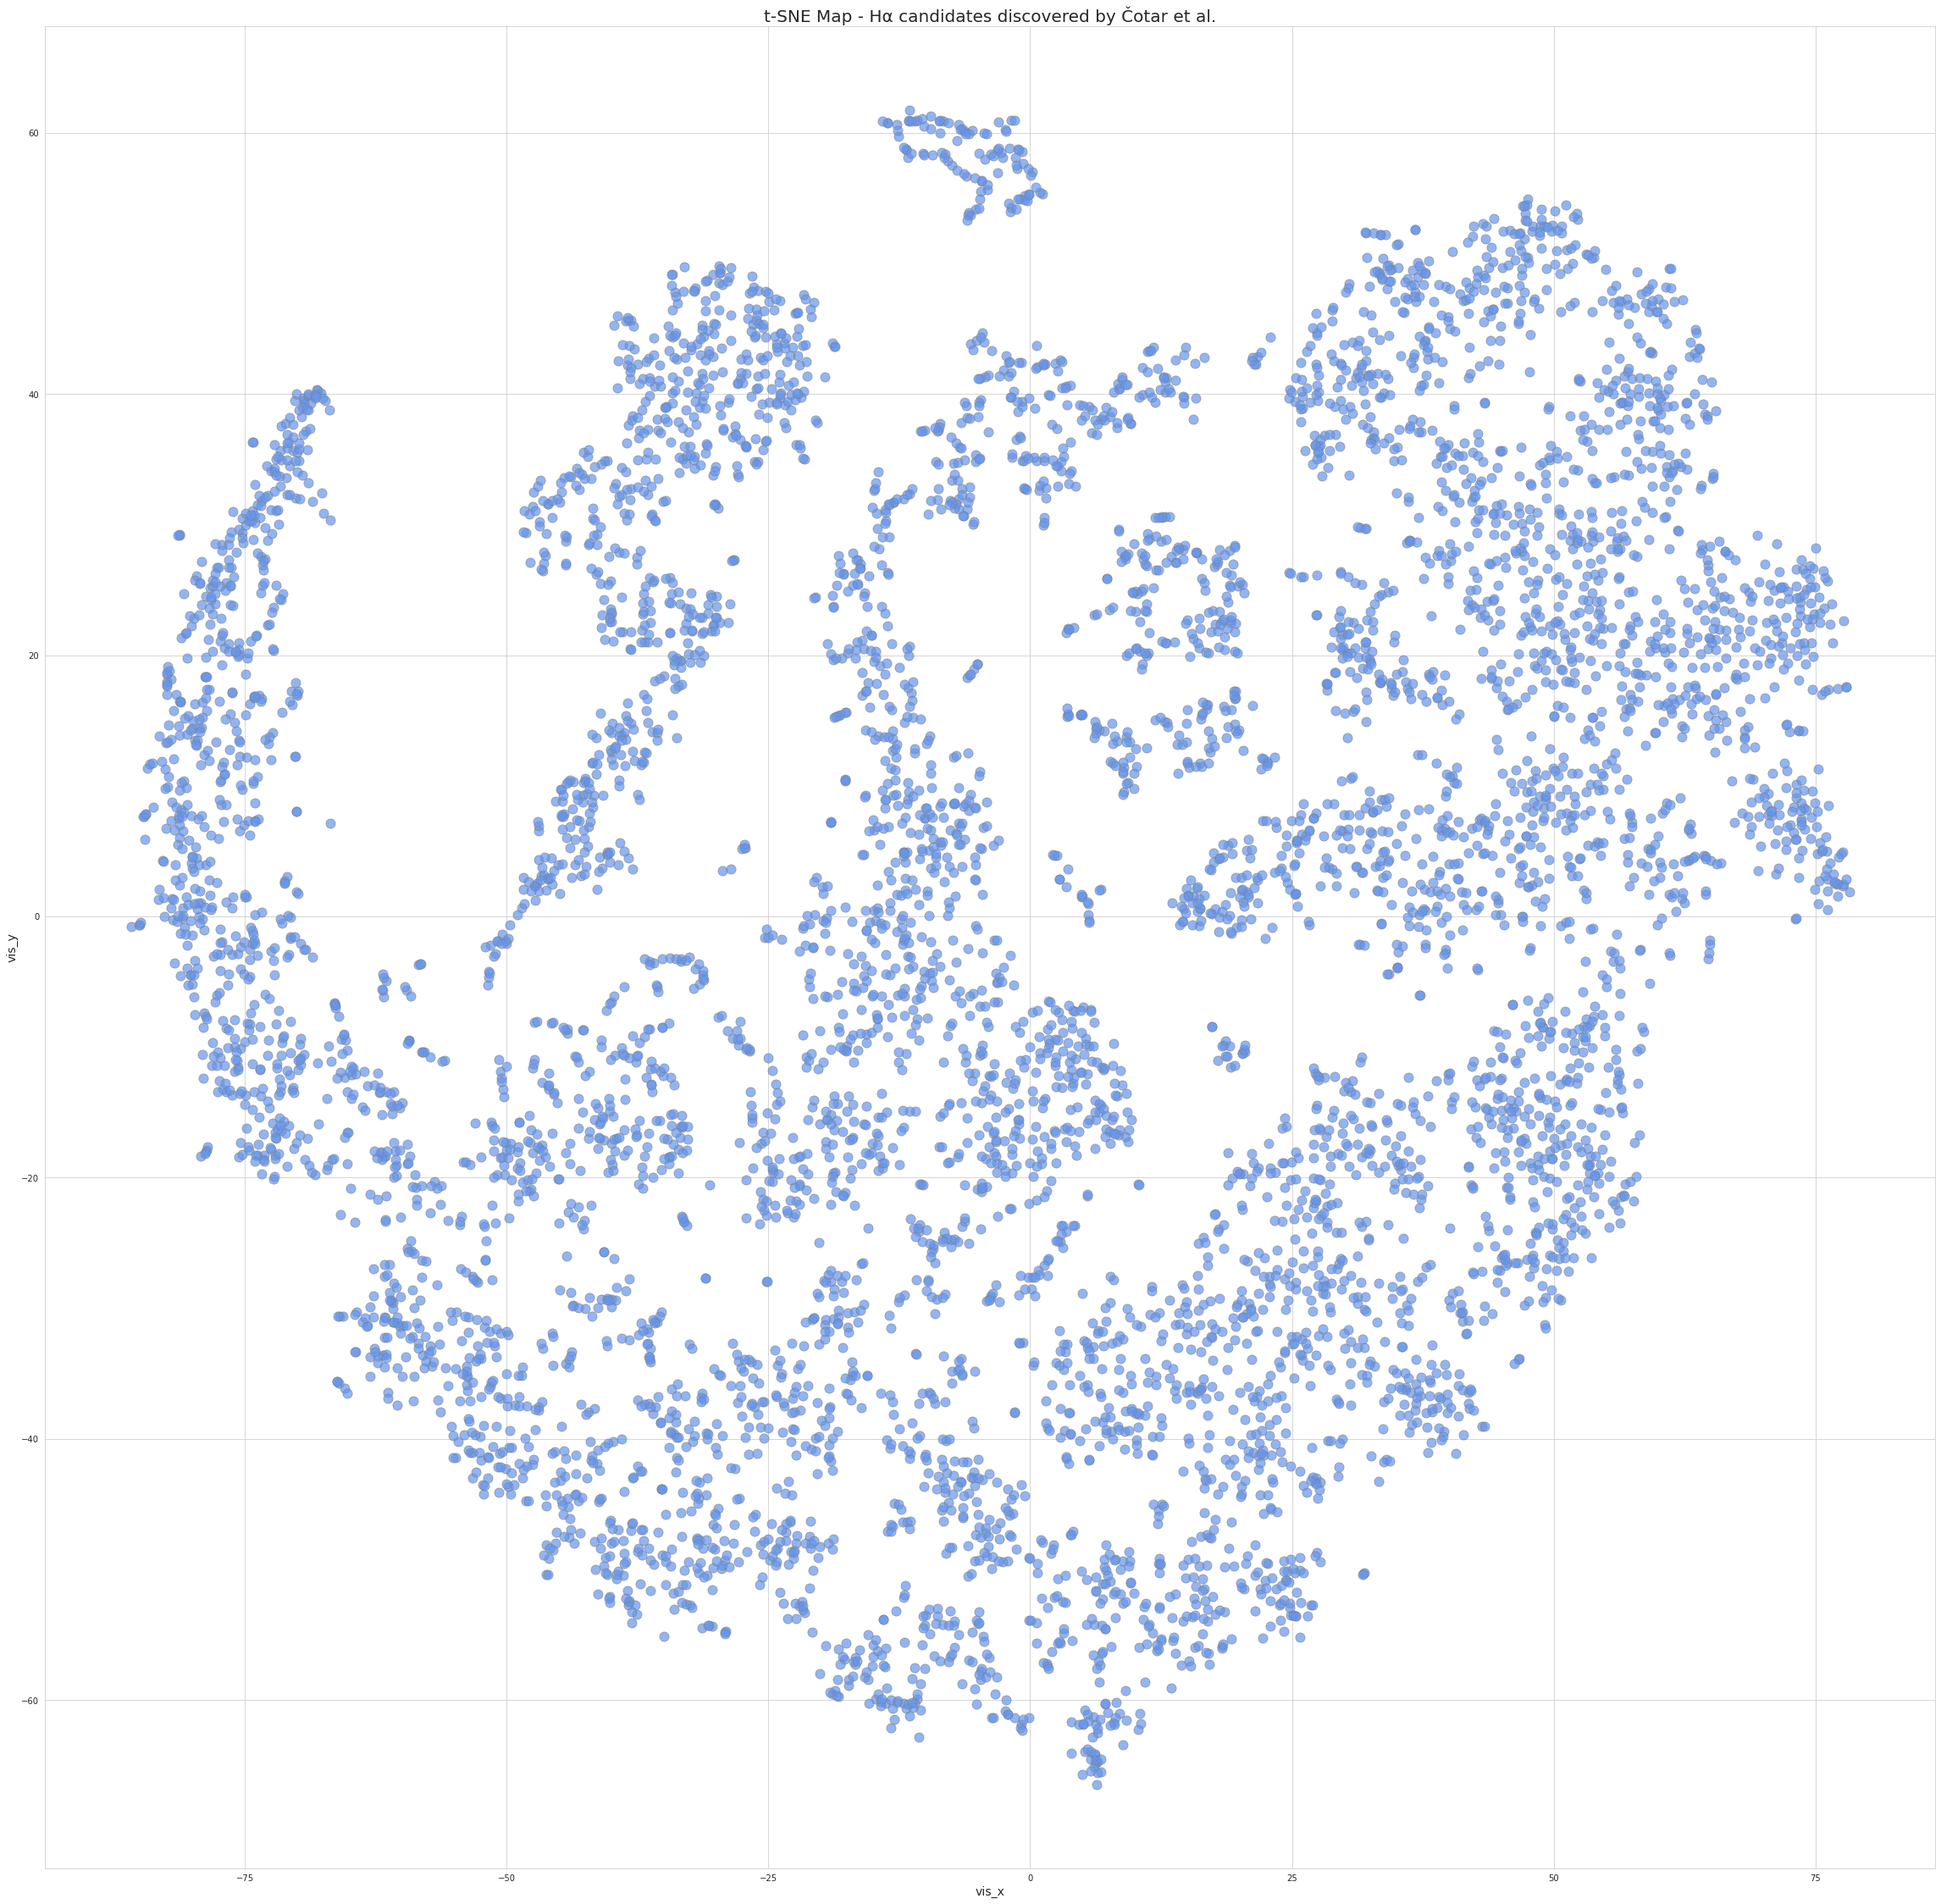
\includegraphics[scale=0.12]{figures/t-sne cotar et al.png}
\caption{t-SNE map for H$\alpha$ candidates identified by Čotar et al. in DR3}
\end{figure}

Note that the representation is significantly simpler compared to the prior application of t-SNE to DR3. The ten clustered identified by the DTW based methodology outlined in chapter 4 yields the following map.

\begin{figure}[t]
\centering
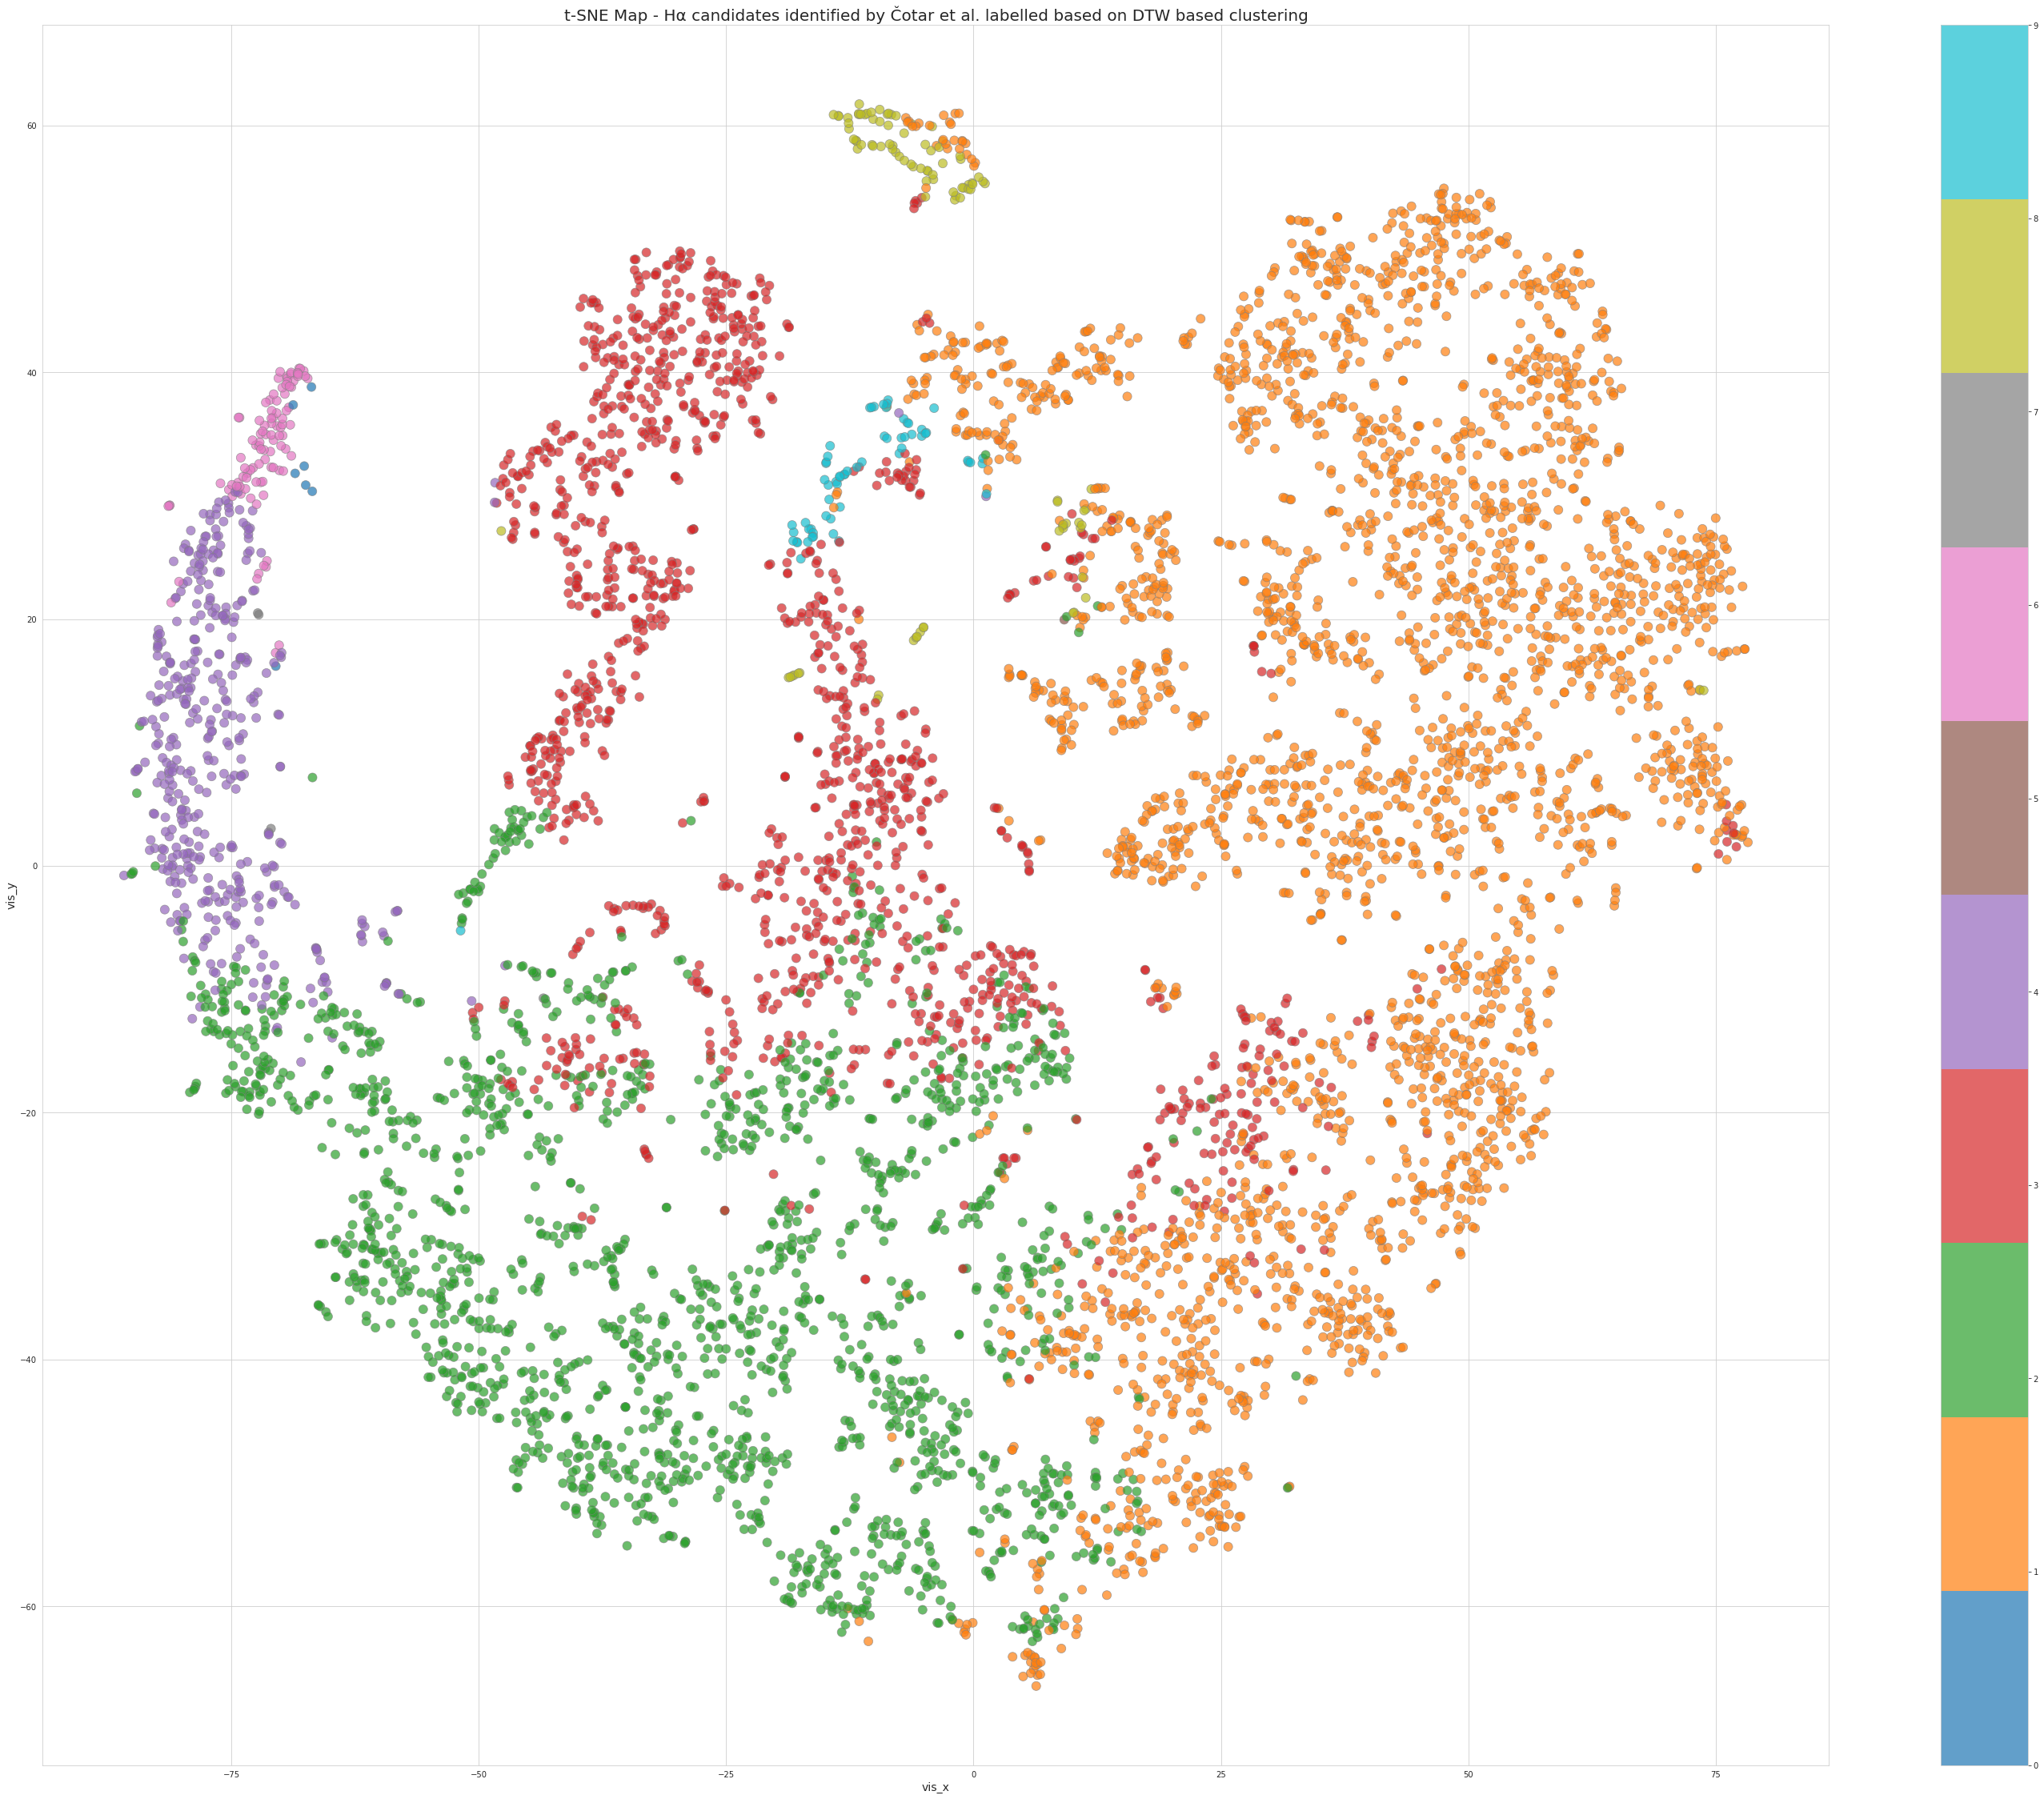
\includegraphics[scale=0.16]{figures/t-sne colored by dtw.png}
\caption{t-SNE map for H$\alpha$ candidates identified by Čotar et al. labelled based on DTW based clustering.}
\end{figure}

Here the P Cygni candidates are represented by cluster 8 and by the colour lime-green while the inverse P Cygni spectra are represented by cluster 9 and the colour teal. Note that cluster 8 appears in two physically separate regions of the t-SNE map and as does cluster 9. Thus it is clear that the application of t-SNE on the H$\alpha$ candidates identified by Čotar et al. does not meaningfully separate P Cygni and inverse P Cygni spectra into distinct regions of the t-SNE map.

% NN
\chapter{Identifying and Classifying Emission-line Spectra: The End-to-end Pipeline}

\section{Drawing Conclusions from Prior Chapters}

The following conclusions can be drawn from the results presented in the preceding chapters:

\begin{enumerate}
    \item The curse of dimensionality presents a significant challenge when working with high-resolution data from million star surveys such as GALAH DR3. 
    \item Dimensionality reduction methods such as t-SNE may not be sufficiently robust at identifying emission-line spectra. Furthermore, the two dimensional t-SNE representation may not be sensitive to the morphological differences between emission-line spectra and non-emission line spectra.
    \item Given a data set with emission-line spectra, DTW-based agglomerative hierarchical clustering can be used effectively to identify and categorise P Cygni, inverse P Cygni and other emission-line spectra.
\end{enumerate}

This chapter builds on these conclusions and presents a proof of concept pipeline for the identification and classification of emission-line spectra. DTW-based agglomerative hierarchical clustering, which  was introduced in Chapter 4, forms the basis of this pipeline. Furthermore, this pipeline relies on the pre-selection of H$\alpha$ emission-line spectra using an autoencoder first introduced by \citet{vcotar2021galah}. In this chapter, the full GALAH DR3 data set will be utilised, as opposed to the much smaller H$\alpha$ emission-line star data set provided by \citet{vcotar2021galah}, which was used extensively in Chapter 4 and Chapter 5.

\section{Identifying H$\alpha$ Emission-line Spectra}

Chapter 2 presented an autoencoder neural network developed by \citet{vcotar2021galah} that is capable of identifying H$\alpha$ emission-line spectra. This method was adapted as a pre-processing step prior to the application of the DTW-based agglomerative hierarchical clustering technique demonstrated in Chapter 4. The autoencoder method is as follows:

The autoencoder learns the latent space representation of non-emission line spectra but \emph{does not} learn the latent space representation of emission-line spectra accurately. This latent space represents each higher dimensional high resolution spectrum as a five dimensional vector. This process is known as encoding. Once the training phase is completed, the autoencoder is fed the total DR3 data set to generate predictions for each spectrum. This process is known as decoding. 

The training data are deliberately biased towards non-emission line spectra (so-called normal or typical spectra). Thus the predicted spectra will match the data for non-emission-line spectra more accurately than for emission-line spectra. The flux difference between a predicted spectrum and its observed (original) data counterpart can be used to flag emission-line stars. This flagging can be accomplished by computing the equivalent width of this "difference spectrum" around the H$\alpha$ line.

\subsection{The Autoencoder Architecture and Training}

The autoencoder architecture presented here is similar to the work of \citet{vcotar2021galah} and maps high resolution spectra of dimension 4,459 to a five dimensional latent space. The popular deep-learning frameworks \texttt{tensorflow} \citep{tensorflow2015-whitepaper} and \texttt{keras} \citep{chollet2015keras} were used to develop the autoencoder.

Each successive dense layer in the neural network reduces the dimensionality of the input layer successively by 75\%, 50\%, 25\% and finally by 10\%. Each layer was activated by the non-linear PReLU function \citep{he2015delving}. The training loss is minimised using the Adam optimiser which performs gradient descent \citep{kingma2014adam}.

\begin{figure}[!htb]
\centering
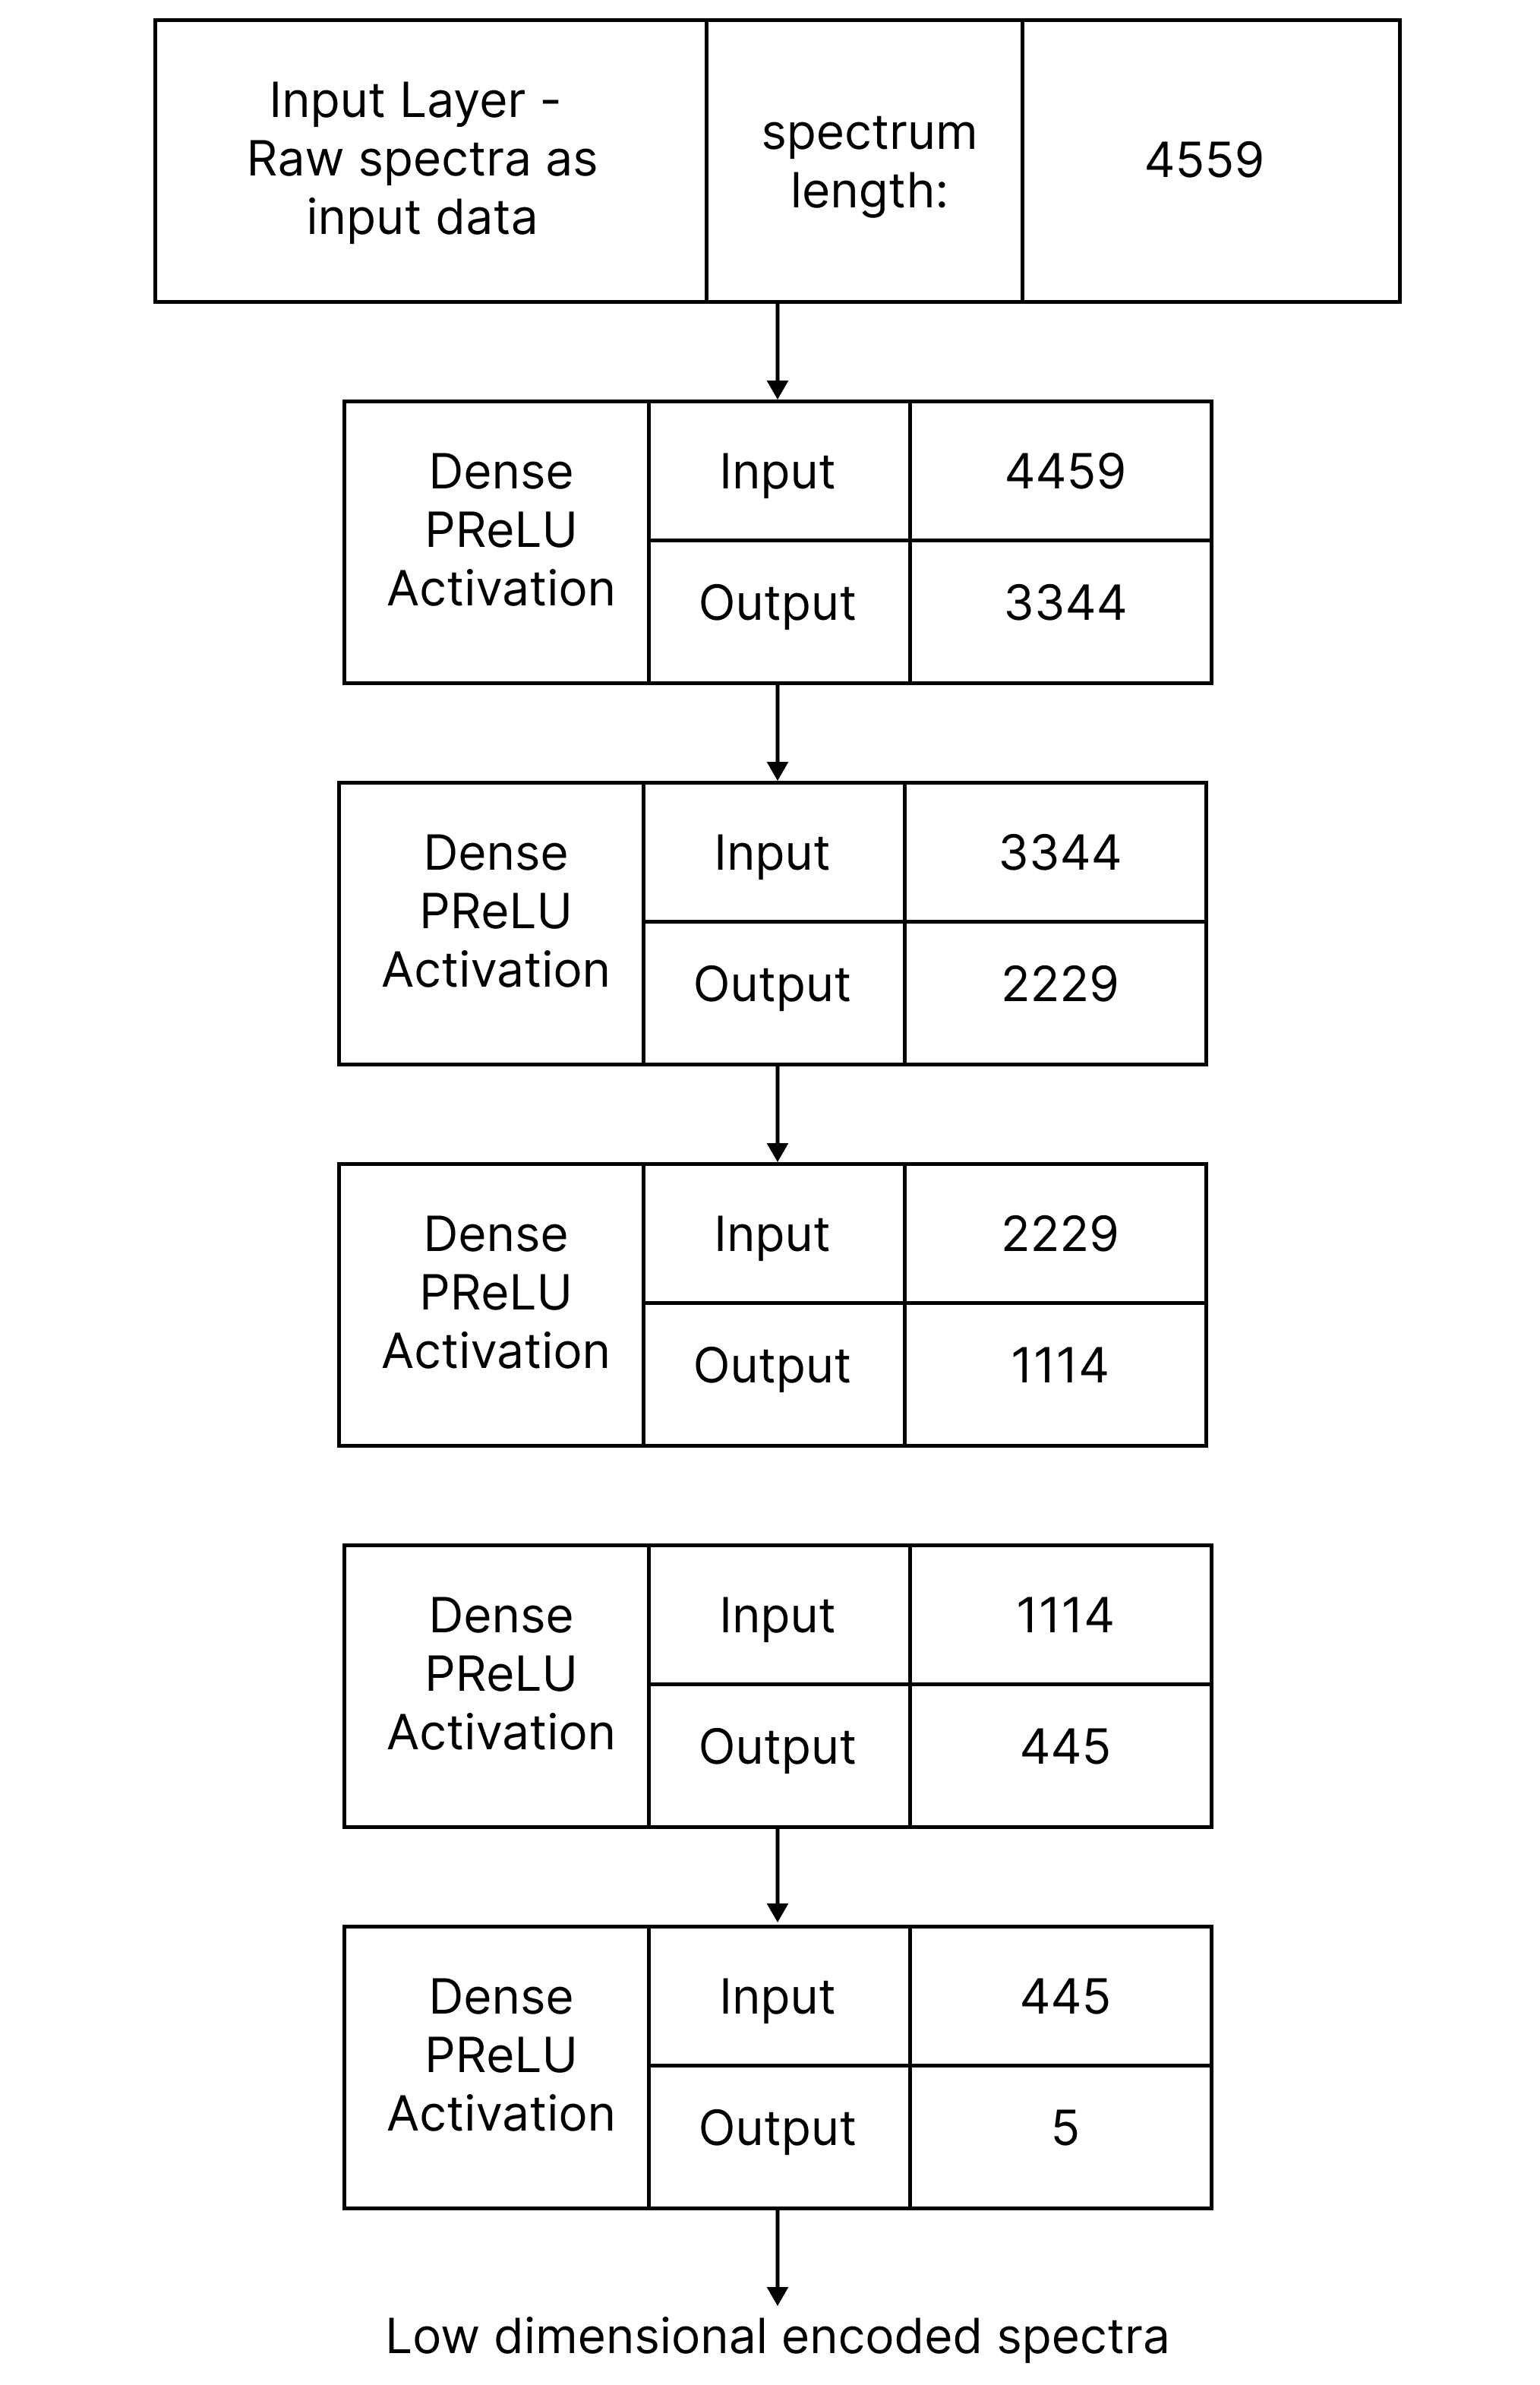
\includegraphics[scale=0.13]{figures/autoencoder diagram.png}
\caption{Visual representation of the encoder. The value in
the right most column of each layer indicates the number of input and output
connections to neighboring layers.}
\end{figure}

\citet{vcotar2021galah} recommended inverting the flux values (1 - normalised flux) prior to training and prediction. Greater training stability was achieved by this inversion. Furthermore, they recommended an epoch size of 350 and a batch size of 40,000 spectra. For validation, 10\% of the samples were selected and set aside. This work followed the same conventions. 

For training, the autoencoder required a training set that is either significantly biased towards non-emission line spectra around H$\alpha$, or better yet, contains exclusively non-emission-line spectra. In order to select these spectra in DR3, the quality criteria recommended by \citet{vcotar2021galah}, \citet{buder2021galah+} and \citet{kos2017galah} were applied. 

While these criteria may not fully guarantee that the autoencoder will be trained exclusively on non-emission line spectra, prior work by \citet{vcotar2021galah} indicated that the criteria are sufficiently robust for the purpose of training this specific network. The Data Central SQL/ADQL catalogue query service was used to retrieve GALAH DR3 \texttt{sobject\_id} values that matched these criteria—namely:

\begin{lstlisting}[language=SQL]
SELECT sobject_id
FROM   galah_dr3.main_star
WHERE  snr_c3_iraf > 30
       AND red_flag = 0
       AND flag_sp < 16 
\end{lstlisting}

\begin{table}[!htb]
\begin{center}
\begin{tabular}{|l|l|}
\hline
\textbf{Criterion}    & \textbf{Rationale}                                                                 \\ \hline
SNR \textgreater 30   & Spectra have reduced noise contamination      \\ \hline
\texttt{red\_flag} = 0         & Select spectra that have no know reduction issues                                  \\ \hline
\texttt{flag\_sp} \textless 16 & Select spectra that do not include known emission-line spectra identified by t-SNE \\ \hline
\end{tabular}
\caption{GALAH DR3 selection criteria for non-emission line spectra for training purposes.}
\label{table:Selection Criteria}
\end{center}
\end{table}
This query returned 396,338 spectra. The red arm data was re-sampled to a common wavelength grid using the method outlined in Chapter 3. The normalised flux was then inverted and used as the training data set.

\begin{figure}[!htb]
\centering
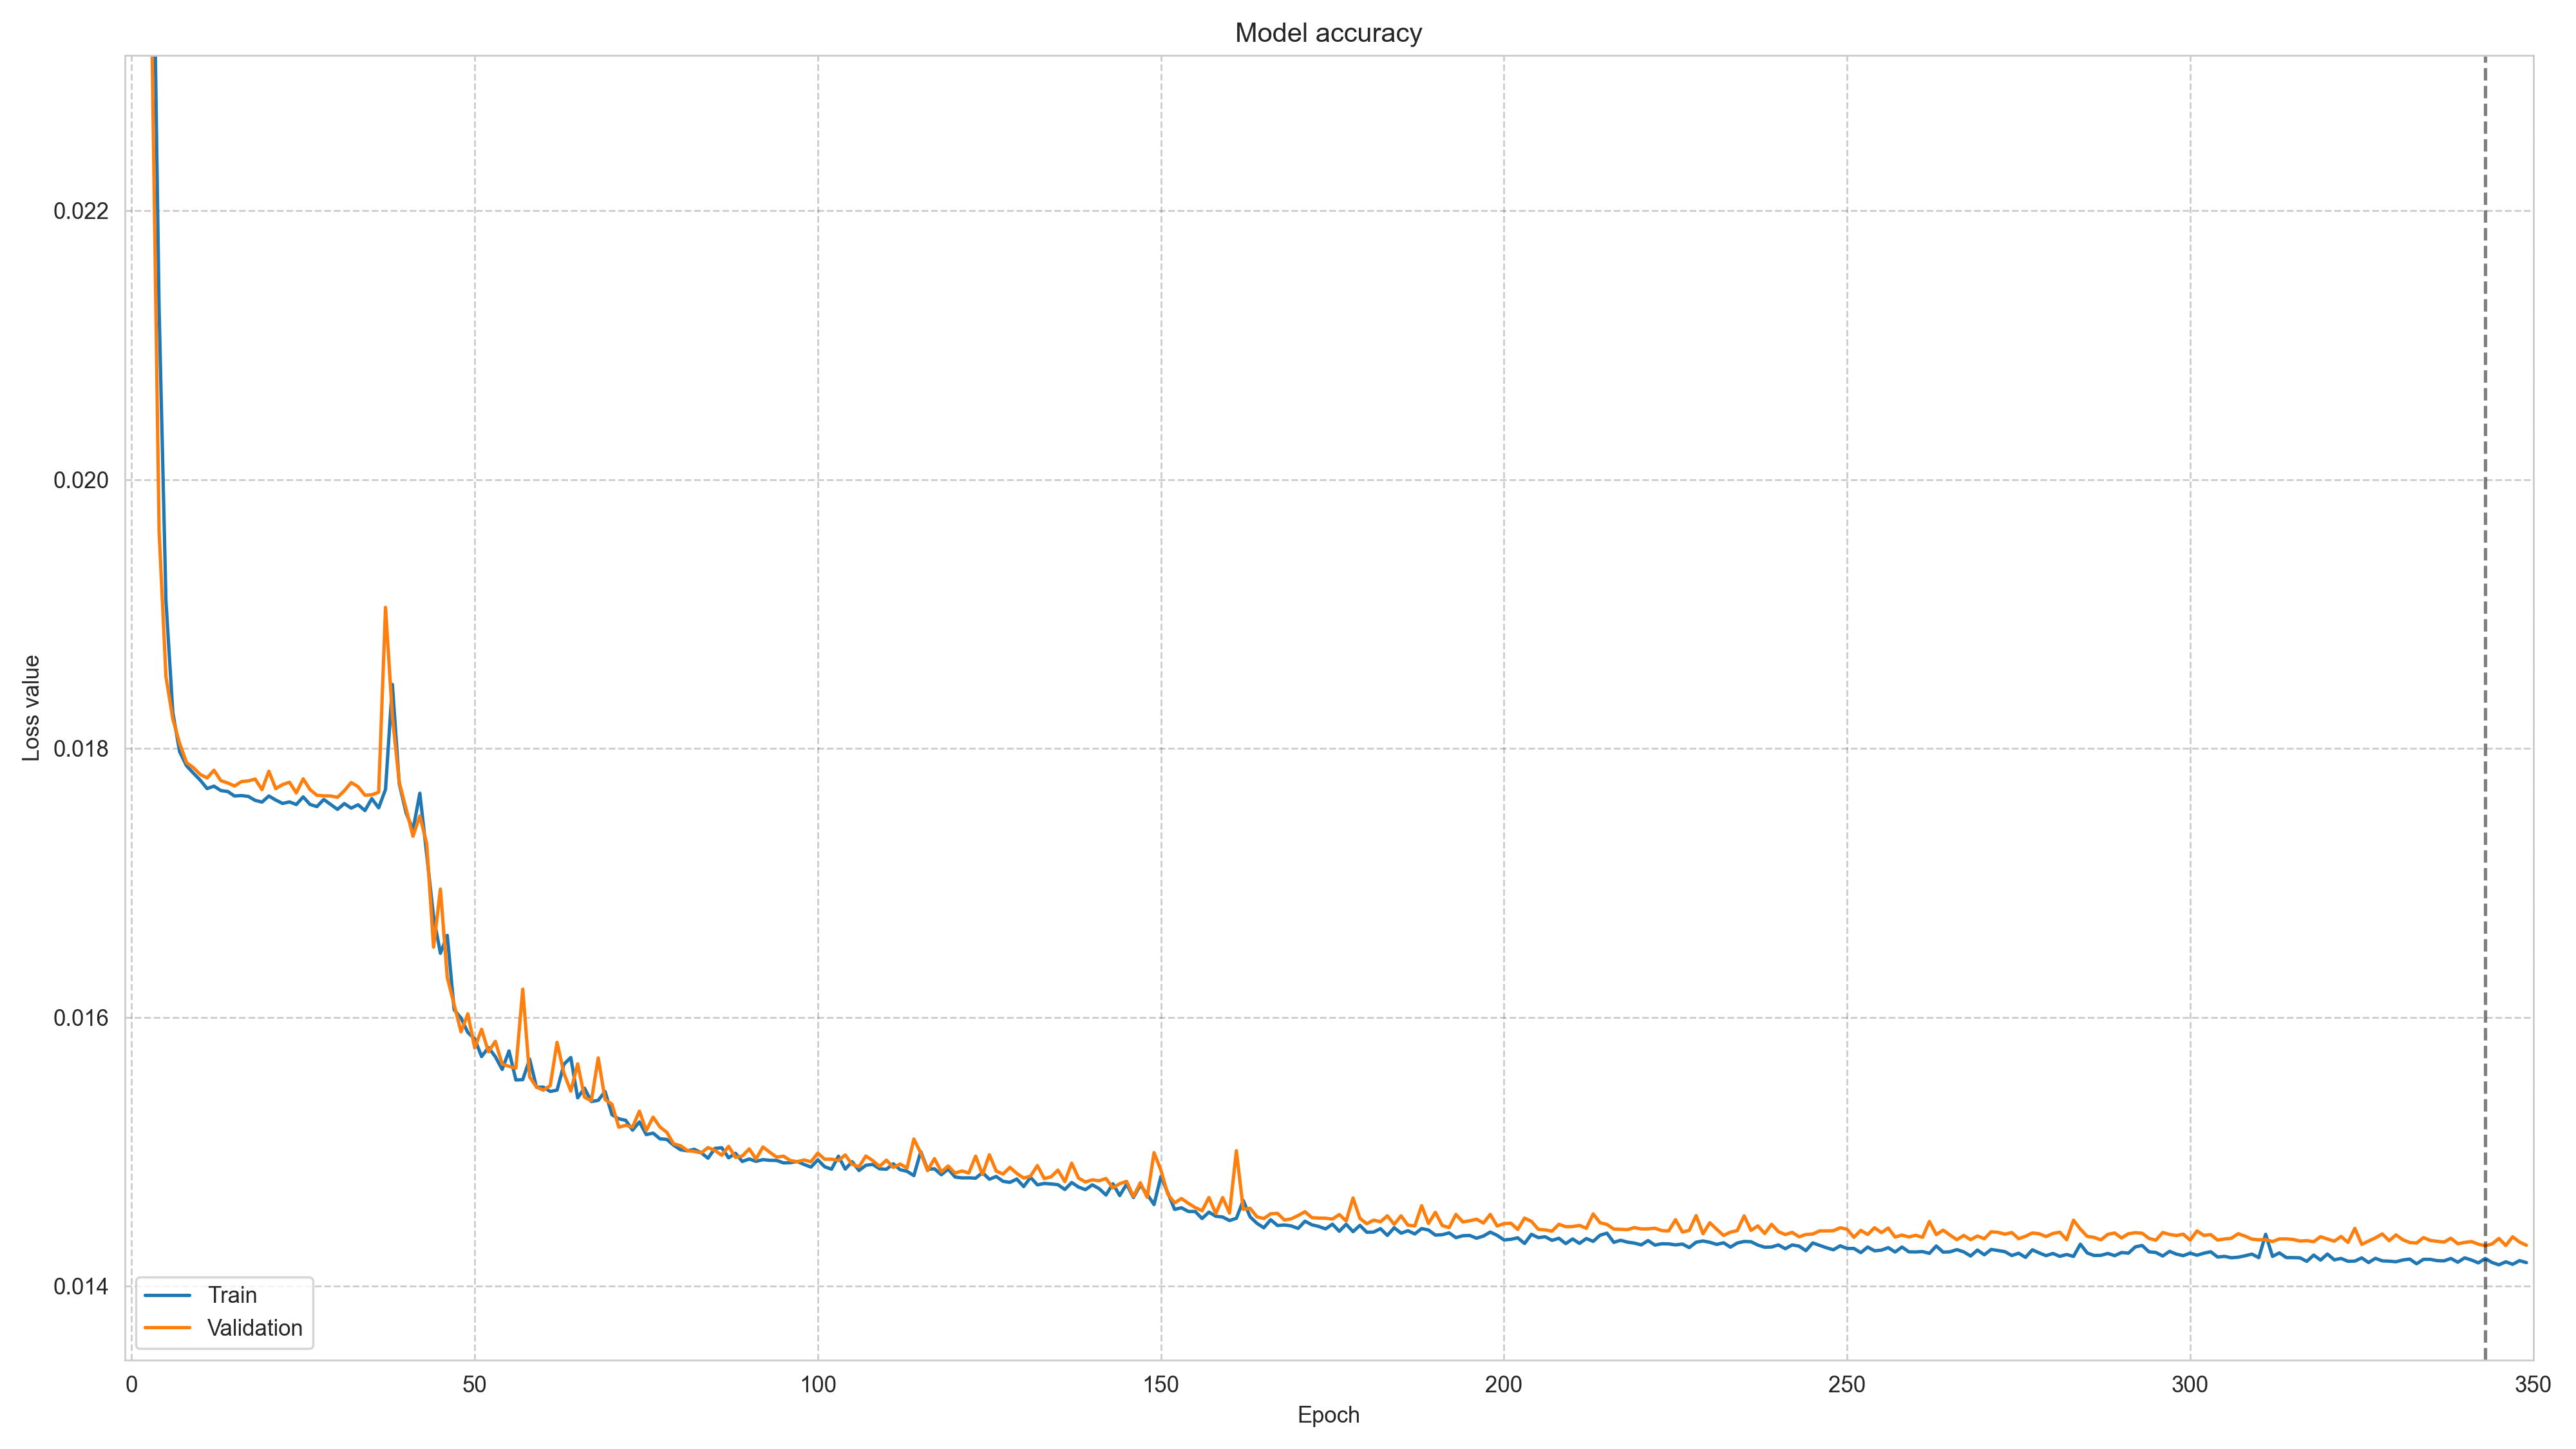
\includegraphics[scale=0.38]{figures/ann_network_loss.png}
\caption{Prediction accuracy of the red arm training data set at different training epochs.}
\label{fig6.2}
\end{figure}
The autoencoder was applied to these data and the prediction error for training was computed as a sum of all absolute differences between the input and output data sets. The results are presented in Figure \ref{fig6.2}, which shows the prediction error as a function of epoch. These results are quite comparable to those presented in \citet{vcotar2021galah}.

It is expected that the autoencoder will perform poorly when attempting to reconstruct or predict emission-line spectra/fluxes. Conversely, it is expected that it will perform well on emission-line spectra. This behaviour has significant implications for the detection of H$\alpha$ emission-line spectra. This is discussed in the next section.

\subsection{Using Difference Spectra to Identify Emission-line Spectra}

Once the autoencoder was trained, data from GALAH DR3 were fed to the network. The network decoded these spectra and provided predictions for each spectrum based on the latent space representation it had learned. Since the input data during the training phase were inverted, for consistency of operation all DR3 spectra were inverted prior to being fed into the network. Predicted results from the autoencoder were also inverted.

The difference spectra between the predicted and the original DR3 spectra (observed spectra) were computed using Formula \ref{formula:6.1}. Presented below are the inverted difference spectra for a known non-emission line spectrum (Figure \ref{fig6.3}) and a known emission-line spectrum (Figure \ref{fig6.4}) in DR3 around H$\alpha$. The emission-line spectrum, which is a P Cygni, was identified from the work presented in Chapter 4. Note that the non-emission-line spectrum produces a difference spectrum with an approximately flat response, while the emission-line spectrum does not. 

\begin{equation}
   f_{difference} = f_{observed} - f_{predicted}
\label{formula:6.1}
\end{equation}

\begin{figure}[!htb]
\centering
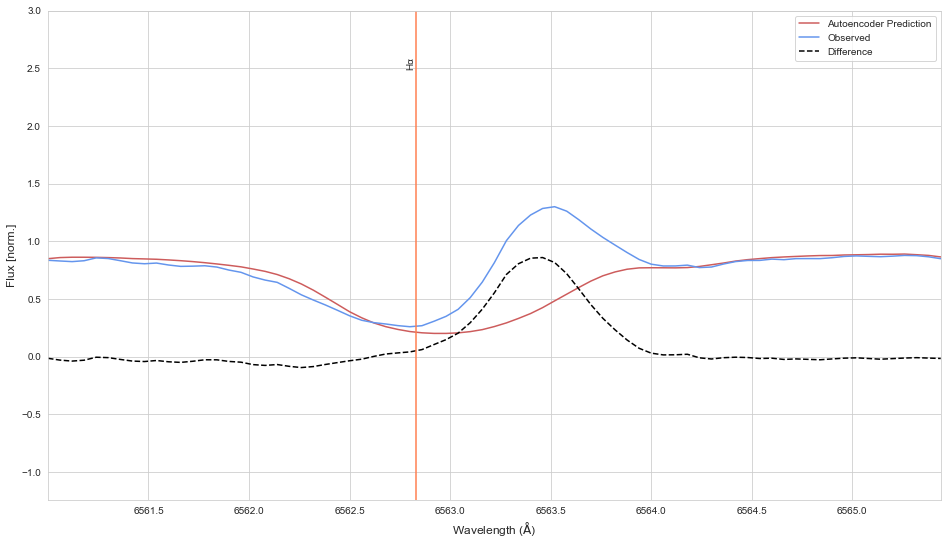
\includegraphics[scale=0.45]{figures/normal difference.png}
\caption{An emission-line spectrum (P Cygni), the autoencoder prediction and corresponding difference spectrum. Note the non-flat response of the difference spectrum. This response can be quantified by calculating its equivalent width.}
\label{fig6.3}
\end{figure}

\begin{figure}[!htb]
\centering
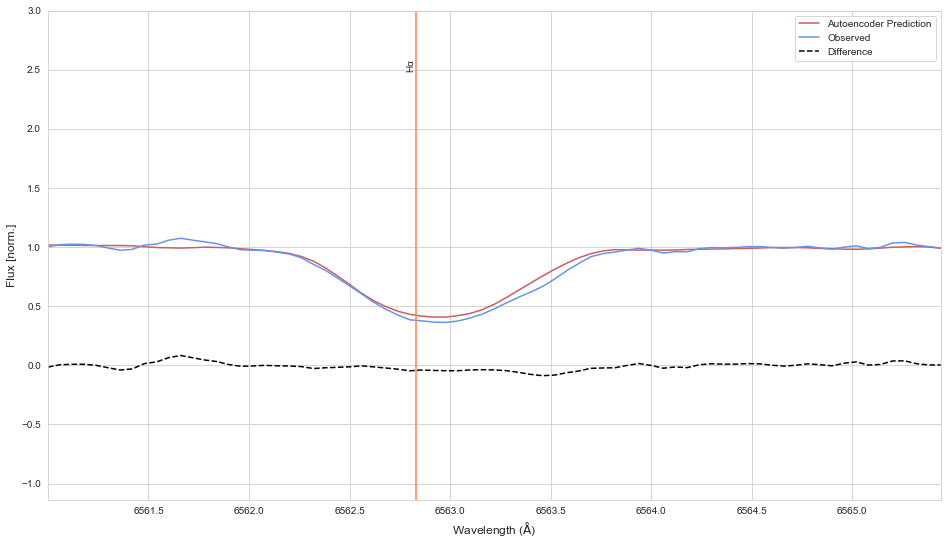
\includegraphics[scale=0.45]{figures/non emission difference.png}
\caption{A non-emission-line spectrum, the autoencoder prediction and corresponding difference spectrum. Note the flat response of the difference spectrum. This response can be quantified by calculating its equivalent width.}
\label{fig6.4}
\end{figure}

The equivalent width within the range 6561\r{A} - 6565\r{A} was determined using the popular Python packages \texttt{astropy} \citep{astropy:2018, astropy:2013} and \texttt{specutils} \citep{specutils}. For consistency, these widths were calculated for the inverted difference spectra. \citet{vcotar2021galah} used an equivalent width cut-off of 0.25 to separate emission-line spectra from DR3. The sensitivity of this cut-off parameter was tested. Selecting a lower threshold for this parameter, such as EW > 0.20,  allows for a wider selection of potential H$\alpha$ emission-line spectra, while a higher threshold such as EW > 0.50 may restrict the selection to only the strongest emitters. The rationale for choosing EW > 0.25 in \citet{vcotar2021galah} was presumably based on a trial and error approach. A similar empirical strategy to fine-tune this parameter and select a reasonable population of H$\alpha$ emission-line spectra resulted in setting EW > 0.22. This value provided the best overall performance. However, this cut-off does not guarantee that the maximum number of H$\alpha$ emission-line spectra was selected. 

Given that \citet{vcotar2021galah} used a different population for their work, the H$\alpha$ emission-line spectra discovered cannot be directly compared to those found in GALAH DR3 using the method above. It can be noted that, due to the inclusion of data from other surveys, only 4,556 out of 10,364 objects identified by \citet{vcotar2021galah} were present in the GALAH DR3 sample, which comprised 396,338 spectra. These 4,556 were also captured and recovered within the H$\alpha$ emission-line spectra discovered using the autoencoder and setting EW > 0.22. The summary statistics for each sample are provided in the Appendix.

\begin{figure}[!htb]
\centering
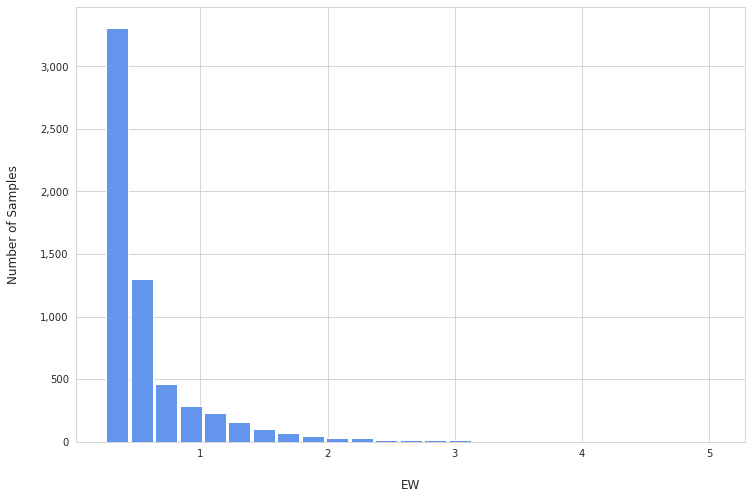
\includegraphics[scale=0.50]{figures/EW hist.png}
\caption{The equivalent width (EW) distribution of the inverted difference spectra of the emission-line spectra identified in GALAH DR3. Here EW > 0.22.}
\end{figure}


\section{Applying Dynamic Time Warping and Agglomerative Hierarchical Clustering}

Once the H$\alpha$ emission-line spectra were selected, the data were passed to the next step of the analytics pipeline. The DTW distance matrix was computed for each spectrum, ensuring that only masked data were presented to the \texttt{FastDTW} algorithm \citep[the masked region being 6561\r{A} - 6565\r{A};][]{traven2017galah}. As mentioned in Chapter 4, this approach significantly reduces run-time and computational complexity. 

\begin{figure}[!htb]
\centering
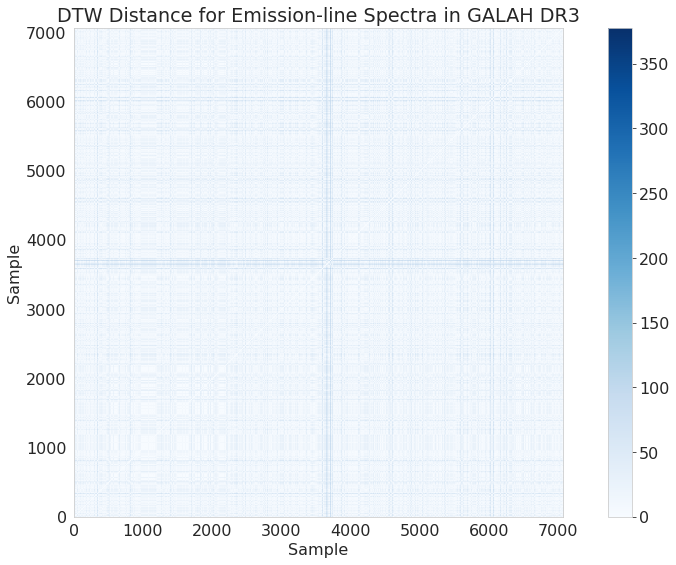
\includegraphics[scale=0.50]{figures/dtw distances dr3.png}
\caption{Pairwise DTW distances for emission line spectra identified in DR3. Darker colours indicate samples that are dissimilar.}
\end{figure}

\begin{figure}[!htb]
\centering
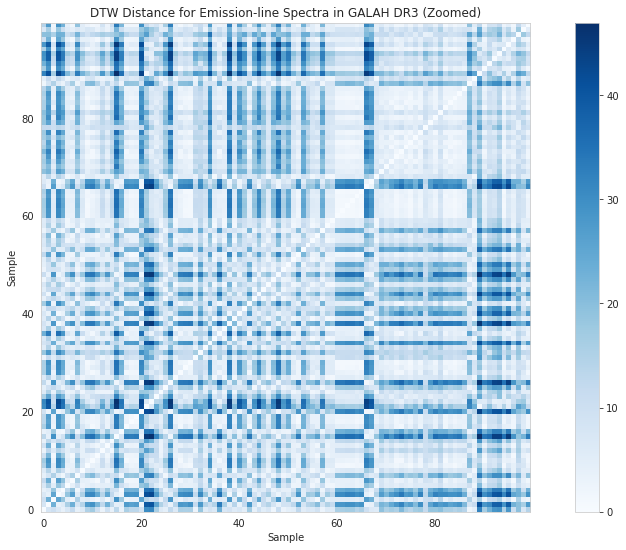
\includegraphics[scale=0.50]{figures/dtw distances dr3 zoomed.png}
\caption{Pairwise DTW distances for emission line spectra identified in DR3 (zoomed). Darker colours indicate samples that are dissimilar.}
\end{figure}

Once the distance calculation was completed, agglomerative hierarchical clustering was performed ensuring complete linkage. At this stage, this work deviated from the number of clusters used in Chapter 4; for one thing, many of the H$\alpha$ emission-line spectra identified in the previous stage of the pipeline exhibited noticeably more complex emission-line morphologies than those identified by \citet{vcotar2021galah}. 

This richer variety of morphologies can be attributed to the fact that the DR3 population is fundamentally different to the survey data used by \citet{vcotar2021galah} This can be demonstrated by observing the number of P Cygni spectra that separate into a cluster as the number of clusters is increased beyond the value (10) used in Chapter 4; with H$\alpha$ emission-line stars identified in the DR3 dataset, the maximum number of P Cygni and inverse P Cygni were separated when the number of clusters was set to 45. This is significantly higher than what was observed in the results presented in Chapter 4. The tree generated by agglomerative hierarchical clustering is thus cut at a depth of 45 (as opposed to 10) for this specific sample for a maximal separation of P Cygni and inverse P Cygni spectra. 

\begin{figure}[!htb]
\centering
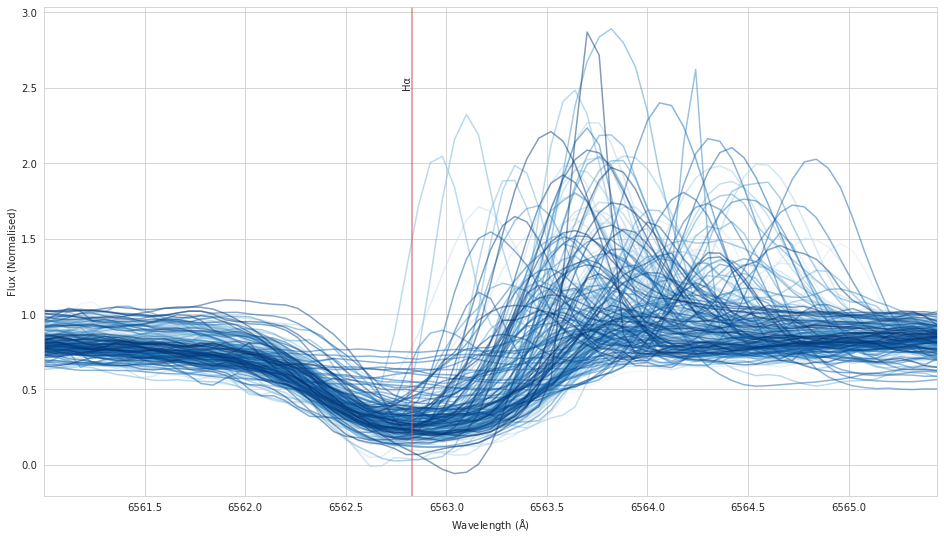
\includegraphics[scale=0.45]{figures/p cygni ensemble.png}
\caption{Ensemble plot of 243 P Cygni spectra identified in DR3 using DTW.}
\end{figure}

\begin{figure}[!htb]
\centering
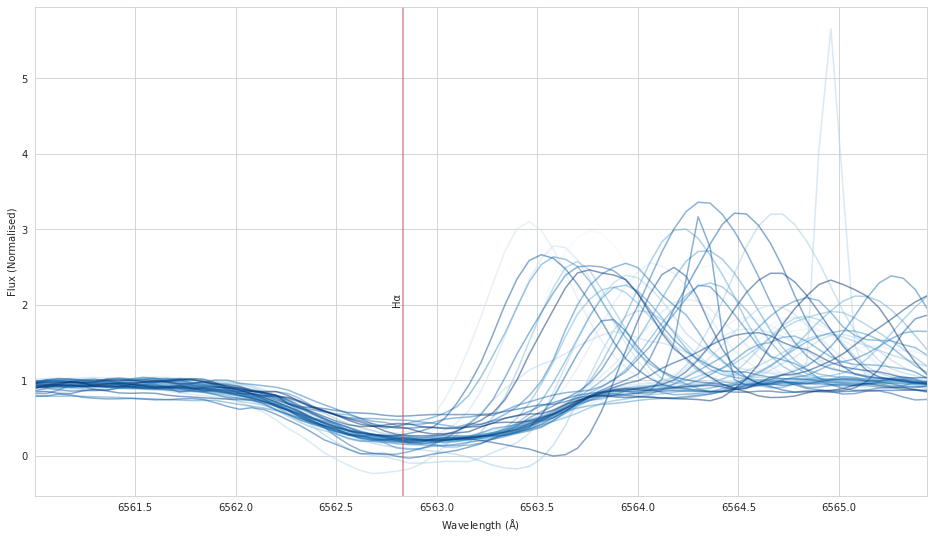
\includegraphics[scale=0.45]{figures/p cugni 2.png}
\caption{Ensemble plot of 53 additional P Cygni spectra identified in DR3 using DTW. These were not included in the main P Cygni cluster but appeared in a separate group, likely due to a less prominent absorption feature blueward of H$\alpha$}.
\end{figure}

\begin{figure}[!htb]
\centering
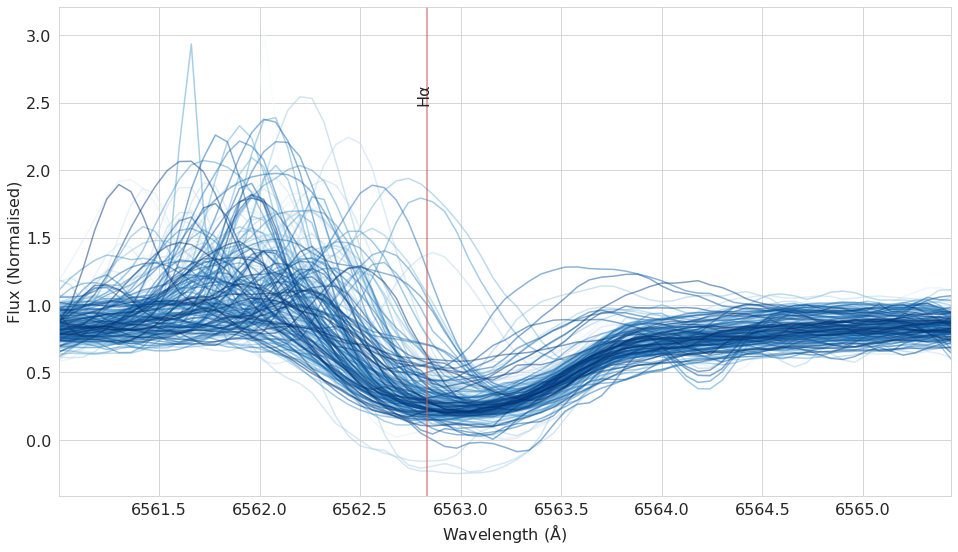
\includegraphics[scale=0.45]{figures/inverse p cygni ensemble.png}
\caption{Ensemble plot of 219 inverse P Cygni spectra identified in DR3 using DTW.}
\end{figure}

The significant advantage of utilizing a higher number of clusters than 10 is that if, as in the case of DR3, more peculiar emission-line spectra are present, they will be separated from the total data set more effectively, i.e., there is no scheme by which these extremely peculiar yet rare spectra can hide in a larger set of data points. These peculiar spectra would form their own minority clusters within the overall hierarchy of the tree generated by the clustering procedure. As far as the author is aware, there exists no precedent in literature for selecting 45 distinct classes for emission-line spectra. However, given that the process outlined here is entirely data driven, it is justifiable, since this value creates maximal separation of P Cygni and inverse P Cygni spectra, as well as the separation of peculiar sub-species in DR3 which have not been classified previously. Additional details of these are provided in the Appendix. Further inspection of key classes were carried out using an interactive plotting tool created by using the \texttt{plotly} package.

\begin{figure}[!htb]
\centering
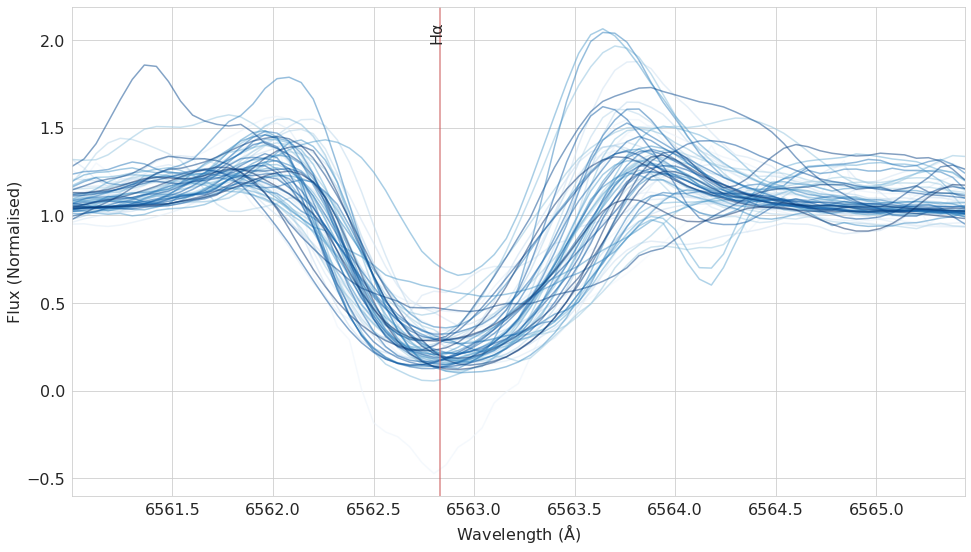
\includegraphics[scale=0.45]{figures/double peak 1.png}
\caption{Ensemble plot of 67 double peaked emission-line spectra identified in DR3 using DTW.}
\end{figure}

\begin{figure}[!htb]
\centering
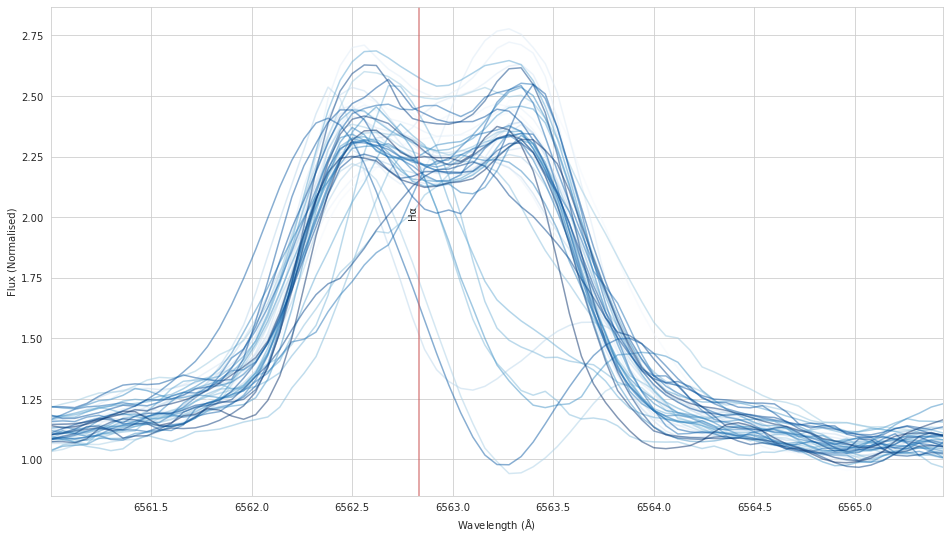
\includegraphics[scale=0.45]{figures/emission on abs.png}
\caption{Ensemble plot of 46 self-absorption type spectra identified in DR3 using DTW.}
\end{figure}

\begin{figure}[!htb]
\centering
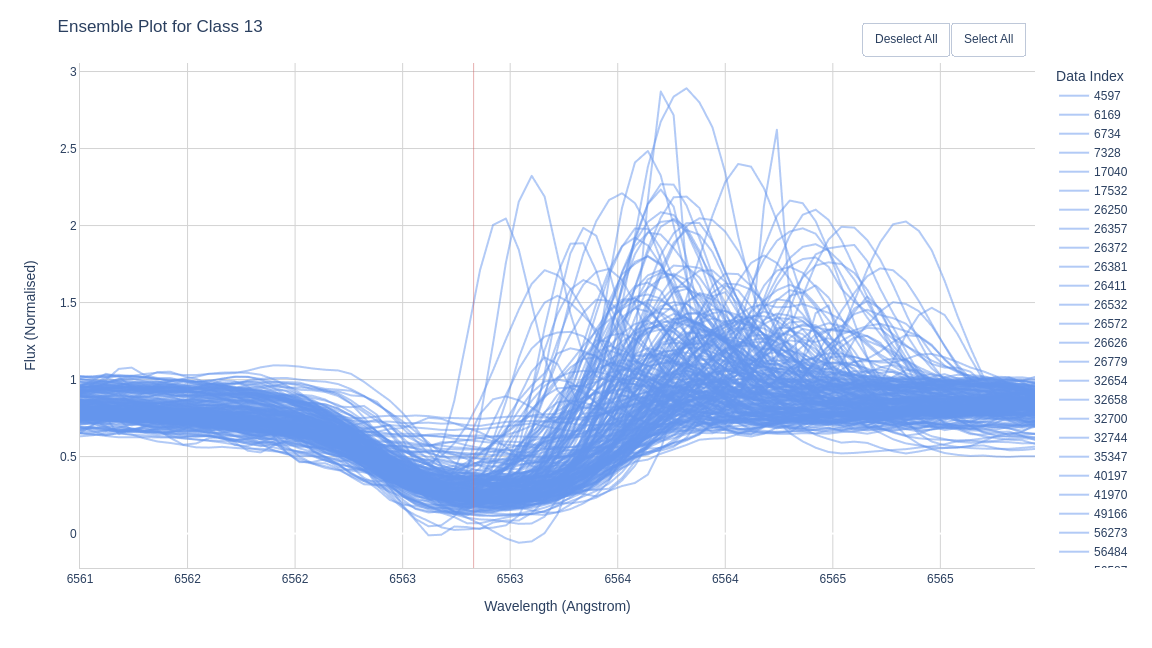
\includegraphics[scale=0.38]{figures/plotly image.png}
\caption{Inspecting a class of spectra identified by DTW using a \texttt{plotly} plot which changes interactively based on the object selected.}
\end{figure}

\section{Concluding Remarks}

Identifying atypical spectra such as emission-line spectra from a data set that contains a majority of typical spectra is a challenging task for machine learning methods. After analysing the requirement and end goals, a unique and powerful combination of methods such as dimensionality reduction, anomaly detection using autoencoders and dynamic time warping was  carefully selected to identify and cluster emission-line spectra in the GALAH DR3 dataset. 

Apart from selecting the number of clusters, the pipeline presented in this work requires significantly less human intervention than other methods in literature. Crucially, it does not require human intervention to manually identify emission-line spectra from a large data set such as GALAH DR3. 

Using these methods, this work was able to identify 296 P Cygni spectra and 219 inverse P Cygni spectra, as well as numerous other classes of stars with H$\alpha$ emission. This leads to the conclusion that, in instances where atypical spectra are hidden in a data set which comprises a majority of typical spectra, this novel approach is able to outperform the machine learning methods presented to date in the literature. 









% Conclusion
\chapter{Conclusion and Future Work}

\section{Conclusion}

Given the deluge of spectroscopic data from modern surveys, manual methods, rule based methods and certain machine learning methods may not be suitable to address the twin problems of identification and classification of non-typical spectra such as H$\alpha$ emission-line stars. The prior chapters demonstrated that these challenges can be overcome using a combination of dimensionality reduction, anomaly detection and spectral morphology based clustering that makes use of dynamic time warping and agglomerative hierarchical clustering. 

The methods presented in this work provides a significant advantage over more recent methods that rely on manual human intervention to identify and classify P Cygni, inverse P Cygni and other species of emission-line spectra\cite{zhang2021catalog}\cite{zhao2012lamost}. In addition to requiring minimum human intervention when setting the machine learning parameter, a key advantage is that these methods do not require a labelled training data set, thus reducing the need for human intervention further.  This work demonstrated that if the code, data structures, algorithms and strategy are picked carefully, emission-line spectra can be identified and classified with reasonable computational efficiency with complexity $O(N)$ without requiring a human being to review thousands and potentially hundreds of thousands of spectra.

The autonencoder used in this work functions as an anomaly detector and is capable of flagging spectra with emission-line features. This is a mature and well established methodology in domains such as credit card fraud detection. This approach can be extended to other domains in astronomy that require the detection of atypical signals from a large volume of more typical signals. Dynamic time warping is a well established signal processing and machine learning method that is sensitive to shapes and morphologies of signals over other features and consequently can be extended to other domains in astronomy where the morphological features of a signal play a dominant role over other features. To this author's knowledge, casting spectra as time series and using DTW has not been used to identify and classify spectra in the literature, and consequently is a novel approach. 

With agglomerative hierarchical clustering, this work demonstrated that the number of clusters and consequently the depth of the hierarchical tree is sensitive to the population mix over which the algorithm is run. In the case of DR3, the maximum number of P Cygni and inverse P Cygni spectra were separated when the number of clusters was set to 45. While the literature informed this work that the number of clusters must be greater than 6 or even 10, determining this value for the emission-line population present in DR3 required an iterative approach of setting the number of clusters and tracking the number of spectra separated from the primary population as P Cygni and inverse P Cygni. While this is not significantly time consuming, it does require human intervention to define and specify a parameter to extract meaningful and useful clusters from the broader emission-line population. 

The larger number of clusters was beneficial in classification of more atypical and exotic spectra. This "over-classification" can be extremely beneficial for researchers that study more exotic emission-line spectra as well as being a useful mechanism to foster further analysis on whether some of the minority classes can indeed be combined with the majority classes that appear at higher levels of the hierarchical tree. These decisions can now be left to the researcher and can be informed by domain knowledge of the peculiar object being studied. For example, it is clear that the clusters presented below can be combined meaningfully into a single P Cygni cluster, thus netting a total of 296 P Cygni spectra. Over classification, prior to merging is thus a beneficial outcome of this approach. 

The method discussed in Chapter 6 is sensitive to a number of factors. Primarily, the type and population of stars captured by a survey has a direct impact on the performance of this method. For example, if a survey is biased towards young stars or in the case of the Gaia ESO survey, open clusters, it is reasonable to expect a high proportion of emission line stars in the raw data. In this scenario the researcher may have to adjust or remove the anomaly detection based autoencoder from the pipeline suggested in Chapter 6. Autoencoders can excel at detecting anomalies in more typical looking data but if the data contains a majority of atypical spectra, the performance of the autoencoder must be evaluated more thoroughly. This work hypothesises that in such scenarios the performance may degrade and as such it may be beneficial to bypass or remove this step and proceed directly computing DTW distances, followed by agglomerative hierarchical clustering. The results from the autoencoder is also sensitive to the equivalent width cut-off criterion described in Chapter 6. Čotar et al. placed this value at 0.25 and the impact of this cut-off on the number off emission-line spectra that can be automatically identified must be modeled. This was beyond the scope of this present work. Similar to the number of clusters, it can be hypothesised that this value is population dependent but posisbly more constrained than the number of clusters.

It is clear that dimensionality reduction techniques such as t-SNE and autoencoders must thus be used judiciously based on the type of population being surveyed. While t-SNE is considered to be a general purposed method, it is less effective at identifying and classifying emission-line stars than the combined application of an autonencoder followed by dynamic time warping and agglomerative clustering. 

\begin{figure}[!htb]
\centering
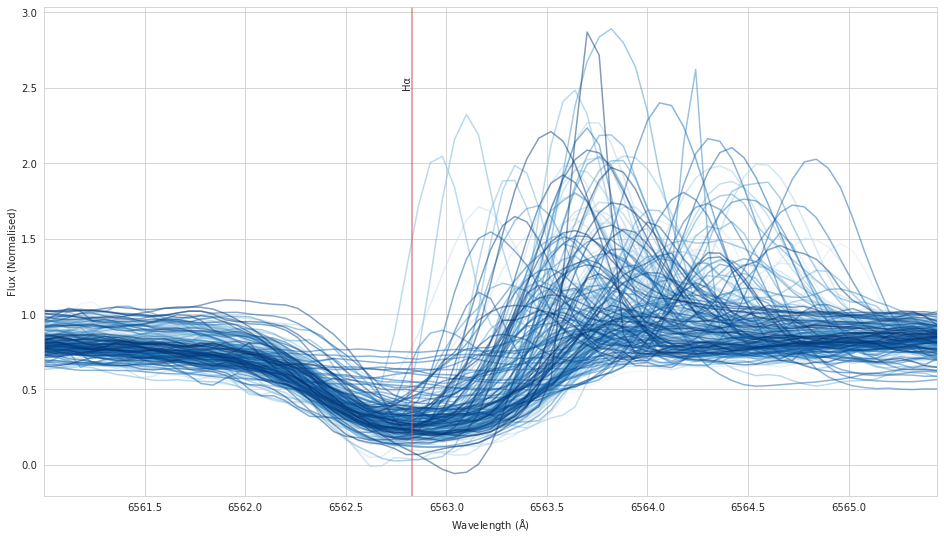
\includegraphics[scale=0.45]{figures/p cygni ensemble.png}
\caption{Ensemble plot of 243 P Cygni spectra identified in DR3 using DTW.}
\end{figure}

\begin{figure}[!htb]
\centering
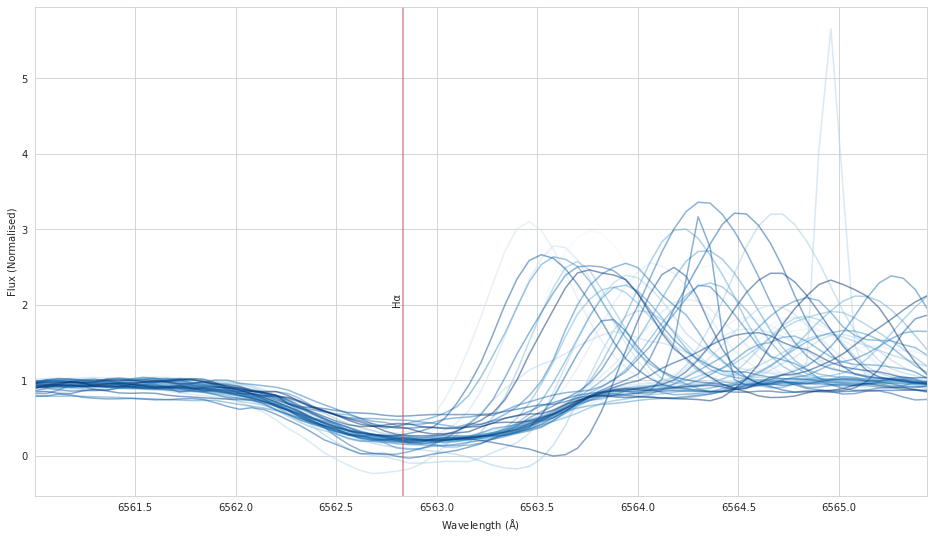
\includegraphics[scale=0.45]{figures/p cugni 2.png}
\caption{Ensemble plot of 53 P Cygni spectra identified in DR3 using DTW. These were not included in the main P Cygni cluster but appeared in a separate group, likely due to less prominent absorption feature near H$\upalpha$. These can be combined with the majority P Cygni cluster to give 296 P Cygni spectra in total.}
\end{figure}

The equivalent width cut-off that selects H$\alpha$ emission-line spectra from the broader DR3 data set is another significant parameter that impacts the final population of classified emission-line stars. The degree to which this population is influenced by this parameter remains unclear. Unlike the number of clusters, there exists no suitbale guiding values for this parameter in the literature apart from the figure presented in Čotar et al. It can be hypothesised that this parameter is linked to the decoding accuracy of the autoencoder but the details of this relationship is beyond the scope of this work.



\section{Future Work and Potential Applications of the Methods Discussed in This Work}

This section presents several future directions and starting points that go beyond this work. 

\subsection{Emission-line Spectra in GALAH DR4}

The GALAH survey has generated more data since DR3. Yet to be released as a public data release, this new data set will contain $\sim$ X spectra. This work will be extended to this next data release. Once these emission-line spectra have been identified and classified, a catalog of emission-line stars, and in particular P Cygni and inverse P Cygni spectra can be released. This requires cross matching the sources with other catalogues such as SIMBAD and Gaia data. Furthermore, as mentioned in the previous section, modelling the sensitivity of the equivalent width cut-off and number of clusters can be carried out with the new data from DR4.

\subsection{Characterising Emission-line Spectra}

Given the number of classes that were identified, it would be extremely useful to characterise each group. More importantly, the stellar parameters of these members deserve reevaluation as the spectra deviate significantly from more typical spectra. It is expected that the stellar parameters for these objects that have already been determined by more standard pipelines may have higher uncertainties compared to those of more typical spectra. Parameters such as effective temperature and stellar masses can be reevaluated for these emission-line spectra outside the primary pipelines. Furthermore, it would be useful to compute the inflow and outflow wind velocities of P Cygni and inverse P Cygni spectra. Expanding the binary mask that was applied to isolate the region near the H$\upalpha$ region can potentially yield objects that have high wind velocities. The methods presented in this work can be suitably adapted to study these high wind velocity objects.

\subsection{Extending to Other Domains in Astronomy}

Dynamic time (wavelength) warping and agglomerative hierarchical clustering are sufficiently generalised methods and can be adapted to a range of problems and sub domains. For example, they can be used to cluster light curves, gravitational waves and radio spectra. Combined with an anomaly detection mechanism such as an autoencoder, these methods can be used to detect highly specific morphologies and signals hidden in large data sets containing typical (normal or non-anomalous) data. 

\subsection{Exploring Dimensionality Reduction for High Resolution Spectra}

Dimensionality reduction remains an extremely useful tool when analysing high dimensional data and feature spaces, thus serving as a tool to potentially overcome the curse of dimensionality. However, it remains unclear which suitable lower dimensional representation of high resolution spectra is more useful in a particular context or set of problems. For example, in the context of clustering morphologically similar spectra, it can be argued that the 5-dimensional representation of the spectra in a latent space formed by the autoencoder was more discriminatory than the 2-dimensional space formed using t-SNE. 

This raises the question as to whether there are general principles or rules that can dictate these decisions for future work; and if applications where clustering is based on another parameter (e.g. effective temperature or metallicity), which lower dimensional representation will yield the best performance. As the volume and complexity of data from large scale surveys continue to grow, determining the most suitable lower dimensional representation or projection of spectra for a given problem can be extremely useful in reducing the complexity of the data analytics process while also reducing the computing overheads. These and related questions remain unanswered at present.

\subsection{Building Training Data Sets for Supervised Learning}

One of the key hurdles a researcher may face when attempting to identify and classify patterns in data using automated methods and machine learning is the lack of training data. Supervised machine learning methods cannot be used in such circumstances. With this work, hundreds of P Cygni and inverse P Cygni spectra have been identified. Additionally other rare species of spectra have also been identified. These can potentially be used to generate a training set for supervised learning algorithms. Care should be taken however when developing these training data sets. It is often important that the training data set accurately reflects the statistics of the population it is attempting to generalise and represent. Thus approaches like stratified sampling must be incorporated into these efforts for the best overall results. 

\subsection{Identifying Emission-line Stars in the GAIA DR3 Spectroscopic Data}

ADD STUFF ABOUT GAIA HERE

CONCLUDE WITH A CONCLUSION 



%---------------------------------------------------------- 
% APPENDICES
% include chapters as needed (will be numbered differently)
%---------------------------------------------------------- 
\appendix

\chapter{Appendix}

\section{Appendix C - Chapter 6}

\begin{table}[!htb]
\begin{center}
\begin{tabular}{|l|l|}
\hline
\textbf{count} & 7067.000000 \\ \hline
\textbf{mean} & 0.532952 \\ \hline
\textbf{std} & 0.444046 \\ \hline
\textbf{min} & 0.220042 \\ \hline
\textbf{25\%} & 0.280778 \\ \hline
\textbf{50\%} & 0.388232 \\ \hline
\textbf{75\%} & 0.562633 \\ \hline
\textbf{max} & 5.055410 \\ \hline
\end{tabular}
\caption{EW distribution summary statistics for emission-line stars identified in GALAH DR3}
\label{table:draglift1}
\end{center}
\end{table}

\begin{table}[!htb]
\begin{center}
\begin{tabular}{|l|l|}
\hline
\textbf{count} & 10364.000000 \\ \hline
\textbf{mean} & 0.539950 \\ \hline
\textbf{std} & 0.420590 \\ \hline
\textbf{min} & 0.250070 \\ \hline
\textbf{25\%} & 0.298572 \\ \hline
\textbf{50\%} & 0.392470 \\ \hline
\textbf{75\%} & 0.592625 \\ \hline
\textbf{max} & 5.369496 \\ \hline
\end{tabular}
\caption{EW distribution summary statistics for emission-line stars identified by Čotar et al. (various surveys).}
\label{table:draglift1}
\end{center}
\end{table}

\begin{figure}[!htb]
\centering
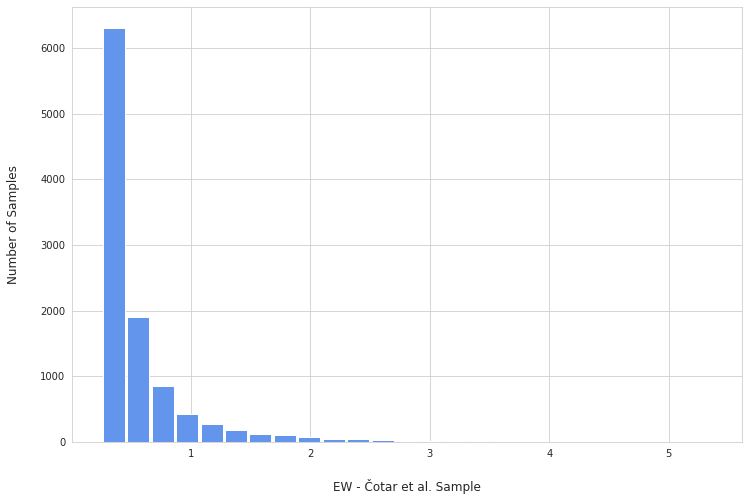
\includegraphics[scale=0.50]{figures/EW hist cotar.png}
\caption{The equivalent width (EW) distribution of the inverted difference spectra of the emission-line spectra provided by Čotar et al. Here EW > 0.25. Note that this sample contains additional spectra not in GALAH DR3.}
\end{figure}






%---------------------------------------------------------- 
% BACK
% list of symbols / references / index etc
%---------------------------------------------------------- 
\backmatter

% your thesis may not need this, so comment out or delete the following line
%\chapter{List of Symbols}

% please change this list to suit your thesis

The following list is neither exhaustive nor exclusive, but may be helpful.
\begin{list}{}{%
\setlength{\labelwidth}{24mm}
\setlength{\leftmargin}{35mm}}
\item[$a$, $b$, $c$, $d$\dotfill] annihilation operators
\item[$a^\dagger$, $b^\dagger$, $c^\dagger$, $d^\dagger$\dotfill] creation
operators
\end{list}


% Bibliography, in BibTeX format (the references.bib file)

\bibliography{references}

\printbibliography

\end{document}
